%%%%%%%%%%%%%%%%%%%%%%%%%%%%%%%%%%%%%%%%%
% Formal Book Title Page
% LaTeX Template
% Version 2.0 (23/7/17)
%
% This template was downloaded from:
% http://www.LaTeXTemplates.com
%
% Original author:
% Peter Wilson (herries.press@earthlink.net) with modifications by:
% Vel (vel@latextemplates.com)
%
% License:
% CC BY-NC-SA 3.0 (http://creativecommons.org/licenses/by-nc-sa/3.0/)
% 
% This template can be used in one of two ways:
%
% 1) Content can be added at the end of this file just before the \end{document}
% to use this title page as the starting point for your document.
%
% 2) Alternatively, if you already have a document which you wish to add this
% title page to, copy everything between the \begin{document} and
% \end{document} and paste it where you would like the title page in your
% document. You will then need to insert the packages and document 
% configurations into your document carefully making sure you are not loading
% the same package twice and that there are no clashes.
%
%%%%%%%%%%%%%%%%%%%%%%%%%%%%%%%%%%%%%%%%%

%----------------------------------------------------------------------------------------
%	PACKAGES AND OTHER DOCUMENT CONFIGURATIONS
%----------------------------------------------------------------------------------------

\documentclass[a4paper, 12pt, oneside]{article} % A4 paper size, default 11pt font size and oneside for equal margins

\newcommand{\plogo}{\fbox{$\mathcal{PL}$}} % Generic dummy publisher logo

\usepackage[utf8]{inputenc} % Required for inputting international characters
\usepackage[T1]{fontenc} % Output font encoding for international characters
\usepackage{fouriernc} % Use the New Century Schoolbook font
\usepackage{graphicx} 
%\usepackage[hmarginratio=1:1,top=35mm,columnsep=20pt,total={6in, 9in}]{geometry}
\usepackage[natbibapa]{apacite}

\usepackage[colorlinks,linkcolor=blue,citecolor=blue,urlcolor=blue]{hyperref}
\usepackage{tocloft}
\usepackage{booktabs}
\usepackage{pdfpages} 
\usepackage{float}
\usepackage{siunitx}
\usepackage{ragged2e}
\usepackage{fancyhdr}
\usepackage{subfig}
\usepackage{amsmath}
%\usepackage{nomencl}
%\makenomenclature
%\renewcommand{\nompreamble}{This list describes several symbols that will be later used within this thesis}
 
\pagestyle{fancy}
\fancyhf{}
\rhead{B.J. Norfolk}
\lhead{Final Year Thesis}
\cfoot{\thepage}
\setlength{\headheight}{14pt}
%\usepackage[style=numeric,natbib]{biblatex}
%\addbibresource{sample.bib} 
%----------------------------------------------------------------------------------------
%	TITLE PAGE
%----------------------------------------------------------------------------------------

\begin{document} 

\begin{titlepage} % Suppresses headers and footers on the title page

	\centering % Centre everything on the title page
	
	\scshape % Use small caps for all text on the title page
	
	%\vspace*{1\baselineskip} % White space at the top of the page
	
	%------------------------------------------------
	%	Title
	%------------------------------------------------
	\begin{figure}[H] 
	 \centering
	 
\includegraphics[scale=0.4]{monash_logo.jpg} 
    \end{figure}
    Department of Mechanical and Aerospace Engineering
    
    \vspace{2\baselineskip}
    
	{\Large Honours Thesis}
	

	\vspace*{3\baselineskip} % Whitespace under the subtitle
	
	\rule{\textwidth}{1.6pt}\vspace*{-\baselineskip}\vspace*{2pt} % Thick horizontal rule
	\rule{\textwidth}{0.4pt} % Thin horizontal rule
	
	\vspace{1.5\baselineskip} % Whitespace above the title
	
	{\LARGE Transient Supersonic Jets} % Title
	
	\vspace{1.5\baselineskip} % Whitespace below the title
	
	\rule{\textwidth}{0.4pt}\vspace*{-\baselineskip}\vspace{3.2pt} % Thin horizontal rule
	\rule{\textwidth}{1.6pt} % Thick horizontal rule
	

	
	%------------------------------------------------
	%	Subtitle
	%------------------------------------------------
	

	
	\vspace*{3\baselineskip} % Whitespace under the subtitle
	
	%------------------------------------------------
	%	Editor(s)
	%------------------------------------------------
	
	Author
	
	\vspace{0.5\baselineskip} % Whitespace before the editors
	
	{\scshape\large Brodie James Norfolk} % Editor list
	
	\vspace{2\baselineskip}
	Supervisor
	
	\vspace{0.5\baselineskip} % Whitespace before the editors
	
	{\scshape\large Daniel Edgington-Mitchell} % Editor list
	
	\vspace{2\baselineskip} % Whitespace below the editor list
	
	 % Editor affiliation
	
	\vfill % Whitespace between editor names and publisher logo
	
	\begin{figure}[H] 
	 \centering
	 
\includegraphics[scale=0.6]{ltrac_logo.png} 
    \end{figure}
	
	%------------------------------------------------
	%	Publisher
	%------------------------------------------------
	


\end{titlepage}
\pagenumbering{roman}
\section*{Abstract}
This thesis aims to explore the fundamental fluid dynamics for transient supersonic jets by means of varying the exit flow nozzle geometry and introducing an impingement plate set at $90^{\circ}$ to the oncoming flow. The study of transient supersonic jets has applications in pressure gain combustion (PGC). PGC is a constant volume combustion process applicable to gas turbines that operates by increasing the stagnation pressure entering the turbine via heat released from combustion. Increasing the turbine inlet pressure allows for considerably more work to be extracted when the turbine expands the flow back to the free stream pressure. The unique design presented in PGC engines predicts 
possible advances in thermodynamic efficiencies leading to significantly lower fossil fuel consumption. The experiment undertaken compares flow regimes of NUMBER and NUMBER Mach numbers for each nozzle geometry at impingement plate positions of 1 and 4 inner nozzle diameters. Transient jet impingement has previously been studied, although it is absent of extensive, repeated experiments, high quality schlieren, and variable exit geometry. This thesis aims to address absences in the literature and explore in detail the shock-vortex interaction during jet impingement. The fundamental fluid dynamics under investigation are; nozzle geometry effects on the shock-vortex interaction and jet impingement, and Mach number variations on all of the latter. 
\newpage
\section*{Acknowledgements}
The author would like to thank those who provided advice and guidance throughout this project. Particularly Dr. Daniel Edgington-Mitchell who supervised the year long project and gave integral feedback, and Bhavraj Thethy for working tirelessly to prepare a functioning laboratory and contributing useful discussions. The author also wishes to acknowledge fellow undergraduate and graduate students including Thomas Knast, Sam Lock, Anesu Junior Kusangaya, and Marcus Wong for assisting in laboratory development and providing key suggestions. The efforts of the Mechanical Engineering Workshop at Monash University are also appreciated for their work in the manufacturing of facility components. Finally, the author thanks his family and friends for their unwavering support throughout all 5 years of his double degree.
\newpage
\tableofcontents
\newpage
\listoftables
\newpage
\listoffigures
\newpage
\section*{Nomenclature}
%This list describes several symbols that will be later used within this thesis.
%\mbox{}
\begin{table}[H]
\begin{tabular}{ll} \smallskip
$B_p$      & Impinging plate base length, mm          \\ \smallskip
$D_i$      & Nozzle entry diameter, mm                   \\ \smallskip
$D_t$      & Nozzle throat diameter, mm                  \\ \smallskip
$D_f$      & Nozzle exit diameter, mm                    \\ \smallskip
$H_p$      & Impinging plate height thickness, mm          \\ \smallskip
$M_1$      & Ambient Mach number                         \\ \smallskip
$NPR$      & Nozzle pressure ratio                       \\ \smallskip
$P_c$      & Chocked nozzle pressure, Pa                        \\ \smallskip
$P_e$      & Nozzle exit pressure, Pa                        \\ \smallskip
$P_n$      & Nozzle pressure, Pa                        \\ \smallskip
$P_1$      & Ambient pressure, Pa                        \\ \smallskip
$P_4$      & Shock tube driver section pressure, Pa      \\ \smallskip
$P_{\infty}$   & Ambient pressure, Pa                        \\ \smallskip
$T_p$      & Impinging plate thickness, mm               \\ \smallskip
$T_{LED}$      & LED pulse width timing, seconds         \\ \smallskip
$U_i$      & Incident shock wave air velocity, m/s       \\ \smallskip
$U_1$      & Ambient air velocity, m/s                   \\ \smallskip
$U_4$      & Shock tube driver section air velocity, m/s \\ \smallskip
$X_{driver}$      & Shock tube driver section length, mm   \\ \smallskip
$X_{driven}$      & Shock tube driven section length, mm   \\ \smallskip
$X_{image}$      & Image length, mm                      \\ \smallskip
$\gamma_1$ & Ambient specific heat ratio                 \\ \smallskip
$\gamma_4$ & Driver specific heat ratio                  \\ \smallskip
$\theta$   & Exterior nozzle angle, degrees   
\end{tabular}
\end{table}
%\nomenclature{$M_1$}{Ambient Mach number}
%\nomenclature{$P_1$}{Ambient pressure, Pa}
%\nomenclature{$P_4$}{Shock tube driver section pressure, Pa}
%\nomenclature{$U_1$}{Ambient air velocity, m/s}
%\nomenclature{$U_4$}{Shock tube driver section air velocity, m/s}
%\nomenclature{$\gamma_1$}{Ambient specific heat ratio}
%\nomenclature{$\gamma_4$}{Driver specific heat ratio}
 
%\printnomenclature


\newpage
\pagenumbering{arabic}
\section{Introduction} 

\subsection{Motivation}
Understanding transient supersonic jets is integral for the integration of pressure gain combustion in ground and aerospace gas turbine applications. PGC offers a significant gain in thermodynamic efficiencies and subsequent reduction in fossil fuel consumption. The literature adeptly describes the fluid dynamics for a transient supersonic jet propagating from a no nozzle shock tube, and the impingement of a transient supersonic on plates set to varying angles in respect to the flow. However, there is an absence of extensive, repeated experiments, high quality schlieren, and variable exit geometry. This thesis is motivated by absences in the literature and aims to explore in detail, the shock-vortex interaction during jet impingement.

\subsection{Aims}
This thesis aims to explore the fundamental fluid dynamics for transient supersonic jets by means of varying the exit flow nozzle geometry and introducing an impingement plate set at $90^{\circ}$ to the oncoming flow. The propagation and time dependent growth of transient and trailing jet Mach disks will be investigated in an attempt to address absences in the literature, and explore in detail the shock-vortex interaction during jet impingement. The pixel relative velocity of the impinging shock wave for plate and no plate experiments will be extracted from the data in order to define each individual flow regime. The fundamental fluid dynamics under investigation are; nozzle geometry effects on the shock-vortex interaction and jet impingement, and Mach number variations on all of the latter.


\newpage

\section{Background Theory} \label{sec:background}
\subsection{Pressure Gain Combustion}
Gas turbine engines are an integral component for the function of ground based power generation and aircraft engines. They account for a large percentage of power generation world wide. Thermodynamic cycle advances in gas turbine design play an important role in preventing the growth of emissions pollution and prolonged global warming \citep{paxson2018pressure}. Pressure gain combustion (PGC) shown in Figure \ref{fig:pcg} is one possible to method of efficiency improvement. PGC is a constant volume combustion process that operates by increasing the stagnation pressure entering the turbine via heat released from combustion. Increasing the turbine inlet pressure allows for considerably more work to be extracted when the turbine expands the flow back to the free stream pressure. PGC optimises gas turbine thermodynamic cycle efficiency, and has the potential to increase current engine efficiency up to 10\% \citep{gulen2013constant}.

\begin{figure}[H] 
 \centering
 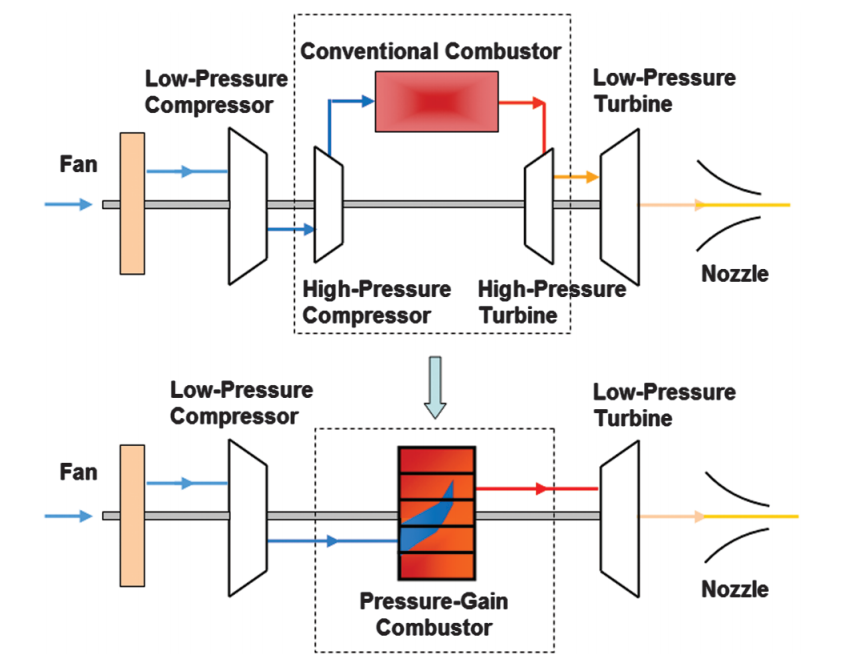
\includegraphics[scale=0.5]{pcg.png} 
 \caption{PCG design concept \citep{akbari2009review}.}
 \label{fig:pcg}
\end{figure}

PGC is at peak efficiency when accomplished through detonation driven combustion, this involves the implementation of detonation waves within the combuster to cause an increase in the temperature and pressure of the fuel-air mixture \citep{eidelman1991review}. During combustion, detonation waves produce flow at supersonic velocities leading to an approximate constant volume and significant pressure gain across the combustor. For supersonic velocities high pressure turbine inlet flow must be steady. A possible method to achieve steady flow at the turbine inlet is via the implementation of a pulse detonation engine \citep{kailasanath2009research} with an equalising plenum chamber. Wear on the first stage of the turbine presents itself as one of the most significant problems of PGC implemetation in current engines. Replacing the combustor in a conventional gas turbine with a pulse detonation combustor (PDC) will result in the propergating detonation waves to converge on the first stage of the turbine. This overtime can lead to concentrated wear on the first stage of the turbine high wear stress points \cite{dean2005operation}. To alleviate turbine wear, the utilization of a high pressure plenum chamber is placed at the exit of the PDC, and creates steady flow conditions effectively shielding the first stage of the turbine from combustion detonations. It remains unclear on how to integrate a pressure plenum into a PDC design. 

\subsection{Transient Supersonic Jet}
The fluid dynamics characterising the governing flow at the exit of PDC is defined as a shock-driven, transient, supersonic jet process \citep{radulescu2007transient}. The governing flow can be classified into several different stages \citep{ishii1999experimental}. The first stage of jet evolution is defined by the diffraction of a shock wave around the corners of the tube exit as shown in Figure \ref{fig:0}. This region is bounded by the curved part of the incident shock, the nozzle lip, and a reflected sound wave. 
\begin{figure}[h]  
\centering
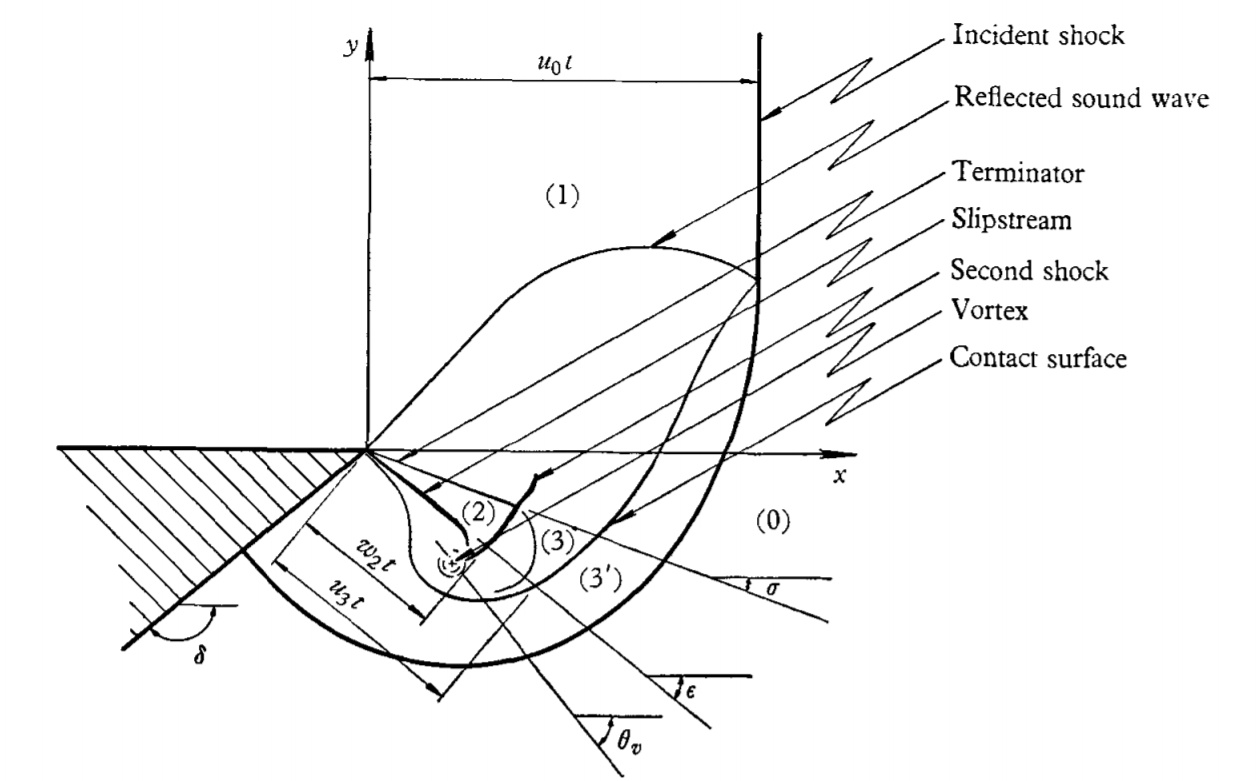
\includegraphics[scale=0.9]{fig0.PNG}
\caption{Features of the diffraction pattern \citep{skews1967perturbed}}
\label{fig:0}
\end{figure}
In the next stage of jet evolution, a vortex ring is generated by the roll-up of the shear layer due to Kelvin-Helmholtz type instabilities along the slipstream at the nozzle lip \citep{elder1952experimental,dora2014role}. Kelvin-Helmholtz instabilities exist within the shock as a result of external perturbations (inhomogeneities in the flow) producing oscillations in the vortex sheet separating fluids with different flow characteristics. This structure propagates down the jet axis, and is simultaneously accompanied by the translation of a curved barrel shock formed initially at the nozzle lip. This instigates the formation of a curved Mach disk for a ratio of the nozzle exit to free-stream pressure exceeding $2.06$ \citep{matsuda1987numerical}. MORE ON MACH DISK

A triple point occurs between the leading edge of the barrel shock, the second shock, and the Mach disk. Given a sufficiently strong jet, a slip surface is generated downstream of the triple point. The first shock cell is formed in the third stage of jet evolution which is marked by the pinch-off phenomenon of the vortex ring, and signals the start of the trailing jet phase \citep{gharib1998universal}. Separation of the vortex ring from the flow structure is driven by Kelvin-Helmholtz instabilities within the shear layer of the trailing jet \citep{zhao2000effects}. The final stage of the supersonic jet is defined by the point at which the transient jet and vortex are no longer joined and the trailing jet forms. This is accompanied by the formation of a quasi-steady shock cell in self-sustained oscillation, radiating strong pressure waves. These four stages of jet evolution are illustrated in Figure \ref{fig:2}.
\begin{figure}[h] 
	\centering
	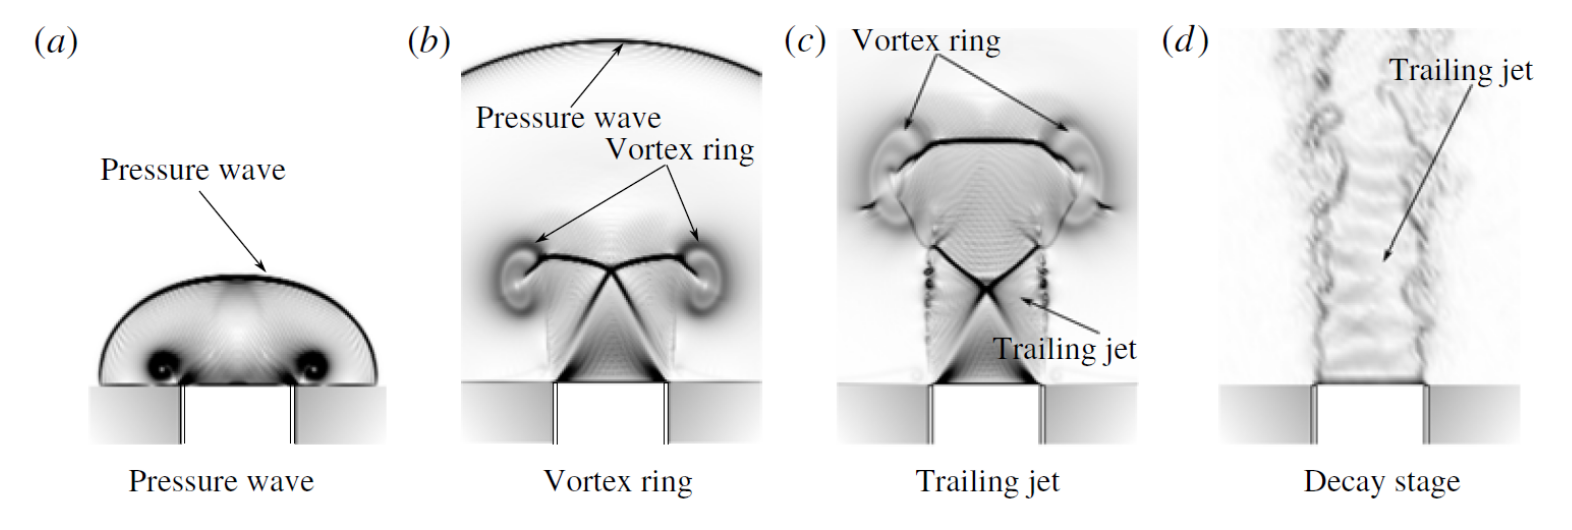
\includegraphics[width=1\textwidth]{fig2.png} 
	\caption{Evolution of the transient supersonic jet. (a) Diffracting shock/Pressure
		wave. (b) Axial translation of the vortex rings, formation of the curved shock and an unsteady Mach disk. (c) Formation of the trailing supersonic jet. (d) Decay of the trailing jet and the end of the transient jet
		process. \citep{fernandez2017compressible}}
	\label{fig:2}
\end{figure}

\subsection{Transient Jet Impingement}
Investigation into the high pressure plenum chamber required for PDEs currently has not been undertaken within the field. However, the flow dynamics is considered analogous to the impingement of a transient supersonic jet on a flat plate. The governing dynamics of transient jet impingment can be classified into serveral stages. The physical process is initially characterised by the reflection of the incident shock wave on the impinging plate. The reflected shock wave propargates back towards the nozzle and interacts with the approaching vortex ring. The central section of the reflected shock wave is captured by the embedded rearward-facing shock at the centre of the vortex ring, and is intensified by the opposing high-speed flow. Simultaneously, the outer section of the shock wave is diffracted by the vortex core. This process results in the formation of a toroidal shock wave which focuses in the trailing jet along the longitudinal axis of flow. The next stage of the fluid dynamics is defined by the impingement of the propagating vortex ring. Initially, as the vortex ring approaches the wall, its propagation velocity decreases and its diameter increases due to the adverse pressure gradient present \citep{szumowski2000starting}. After votex impingement the vortical flow undergoes rapid radial expansion developing a boundary layer on the surface, which slows down the flow and increases the pressure distribution over the plate. After a given duration that is dependent on the initial incident Mach number, the boundary layer separates from the plate and the flow rolls up generating a series of secondary vortices. This also occurs at the thin shear layer present between the jet flow and the exterior fluid as the region rolls up due to Kelvin-Helmholtz instabilities. This produces small interacting secondary vortex rings that propagate towards the plate \citep{minota1997shock}. Cumulative interactions between the primary and secondary wall vortex rings result in a near standing lift off of the pair. The secondary ring subsequently merges with the primary ring, and the weakened newly formed vortex ring continues to translate down the plate. Stages of impingement are illustrated in Figure \ref{fig:4} below.

\begin{figure}[h] 
	\centering
	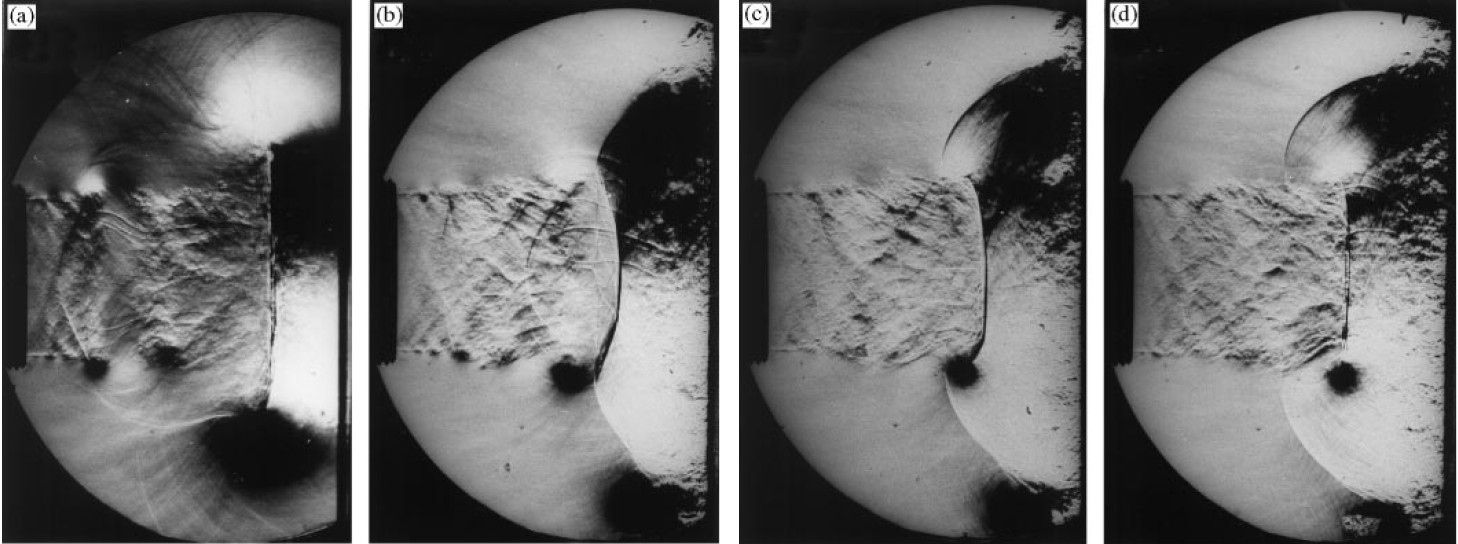
\includegraphics[width=1\textwidth]{fig4.PNG} 
	\caption{Evolution of jet impingement. (a) Impingement of vortex ring. (b) Vortex ring translates down the plate. (c) Secondary vortex formation. (d) Lift-off of votex rings and dissapation. \citep{szumowski2000starting}}
	\label{fig:4}
\end{figure}
For a plate of variable angle, the lower core of the vortex ring impinges initially and generates an asymmetric set of secondary vortices. These new flow structures orbit around the main vortex, creating a temporarily thicker boundary layer at the lower end of the flow field. Again after a period of time, dependent on the incident Mach number, he boundary layer separates from the plate. This results in the vortex ring pivoting on the lower core, undergoing negligible deformation, and propergates towards the surface plate. The upper core then impinges on the plate and the upper wall vortex is generated. This new structure begins to expand radially increasing in thickness due to the remaining jet flow. While simultaneously, the lower wall vortex propagates around the outer limits of the main vortex, stops expanding, and dissipates into a thin structure. The impinging jet continues to feed into the upper section of the flow field generating wall vortices with a thicker upper core. For lower angles of plate alignment, the flow field shows an increase in overall velocity and visible curvature of the vortex ring structure during impingement. The toroidal shock wave that forms as a result of impingement propagates perpendicularly with respect to the surface \citep{mariani2013head}.  

\subsection{The Underexpanded Trailing Jet}
The final stage of a transient supersonic jet is defined by the formation of the trailing jet. The structure of the trailing jet is dependent on the nozzle pressure ratio (NPR) which is a function of pressure at the nozzle $P_n$ and the ambient pressure $P_{\infty}$.

\begin{equation}
NPR = \frac{P_n}{P_{\infty}}
\end{equation}

The underexpanded jet is defined as exhaust jet flow that operates at pressures greater then ambient conditions ($NPR\geq 1$), the degree of under-expansion is dependent on the nozzle pressure and properties of the gas. For the formation of a supersonic underexpanded jet the trailing jet must have a minimum Mach number of 1, this is defined as the chocked nozzle condition and is physically characterised by the presence of a normal shock  at the nozzle exit. The pressure ratio at the chocked nozzle condition is a relation between the exit pressure $P_e$, chocked nozzle pressure $P_c$, specific heat ratio of gas $\gamma_g$, and flow constant A \citep{anderson2010fundamentals}.

\begin{equation}
\frac{P_e}{P_c} = \left(\frac{1}{1-A}\right)^{\gamma_g/(\gamma_g-1)}
\end{equation}
The flow constant A is a relation between the specific heat ratio of gas $\gamma_g$ and an efficiency $\eta$, for an ideal process it is assumed $\eta=1$.
\begin{equation}
A=\frac{1}{\eta}\frac{(\gamma_g-1)}{(\gamma_g+1)}
\end{equation}

A highly underexpanded as shown in Figure \ref{fig:jet} will signify the final stage of a transient supersonic jet propagating for a shock tube. The formation of an underexpanded supersonic jet and its shock cell structure is due to air flow exiting the nozzle at pressures above the chocked condition. Flow exiting the nozzle instantaneously expands and forms expansion fans which angle the jet outwards temporarily expanding the jet boundary. This results in the jet pressure dropping below the jet boundary pressure (ambient pressure) and leads to the expanding flow curving back towards the jet centreline. Mach lines defining the boundary supersonic and subsonic flow reflect off the jet boundary as compression waves, and due to the curvature of the boundary will converge to form a normal shock. This shock cell structure is repeated as compression waves continue to reflect of the jet boundary and form expansion fans. As the pressure ratio decreases the underexpanded supersonic trailing jet becomes subsonic until the exit pressure is equal to the ambient pressure and the jet is no longer present.

\begin{figure}[H] 
	\centering
	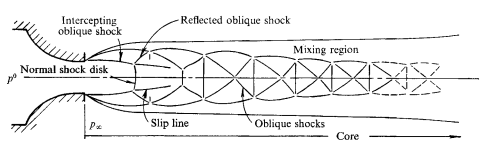
\includegraphics[width=1\textwidth]{jet.png} 
	\caption{Highly underexpanded jet \citep{snedeker1971study}.}
	\label{fig:jet}
\end{figure}

\subsection{Acoustic Noise}
The far-field noise developed by the shock wave-vortex interaction can be decomposed into three components, the sound field due to the formation and evolution of the vortex ring, the reflection shock and vortex ring interaction noise production, and the noise due to impingement of the ring on the plate. The plate-votex ring impingement noise is produced by fluctuating pressure due to the deformation and stretching of the vortex ring, formation and growth of a secondary wall vortex ring, and lifting-off of the primary-secondary vortex ring pair \cite{murugan2010characteristics}.


\newpage
\section{Experimental Methods \& Analysis Techniques}
\subsection{Technical University of Berlin Pulse Detonation Combustion Facility}
The initial imaging processing work conducted in this thesis was tested on experimental data supplied by the Technical University of Berlin's (TBU) pulse detonation combustion (PDC) facility. The PDC facility at TBU consists of a $685mm$ long deflagration-to-detonation transition (DDT) section with a tube diameter of $40mm$, and 825 mm exhaust section with a tube diameter of $30mm$. The DDT supply gas is a combination of hydrogen and air. DDT is initiated with a number of orifice plates, and the leading detonation wave
is tracked using a number of ionisation and pressure sensors placed throughout the exhaust tube. The governing flow dynamics were captured using schlieren measurements positioned in a Toepler Z-Type schlieren system \citep{settles2001schlieren}. The schlieren system is constructed using two 8in parabolic mirrors with a high speed LED providing the necessary light source \citep{willert2012assessment}. The images were captured using a Photron SA-Z camera for converging and diverging nozzles. The experimental layout is shown in Figure \ref{fig:berlin}.

\begin{figure}[H] 
	\centering
	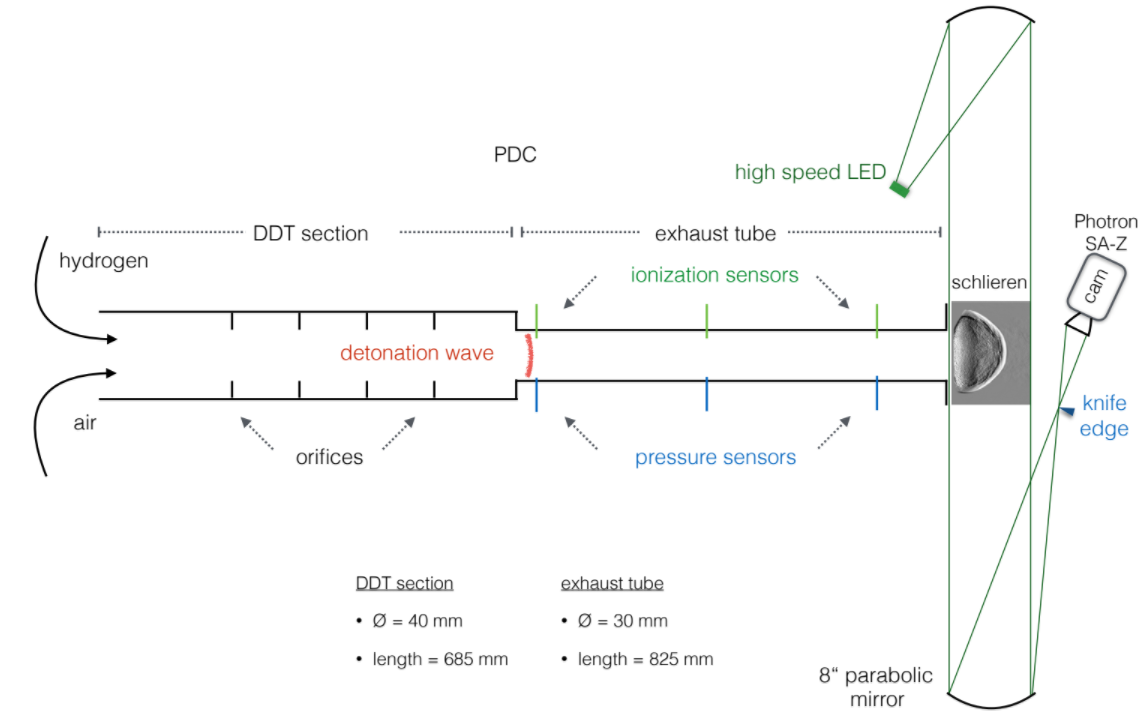
\includegraphics[width=1\textwidth]{berlin.PNG} 
	\caption{Shock tube facility schematic at TUB. Major parts of the
		system have been labelled \citep{bhavberlin}.}
	\label{fig:berlin}
\end{figure}
\newpage
\subsection{Shock Tube Facility}
The experiments presented were conducted in the LTRAC Supersonic Jet Facility. A schematic of the facility is shown in Figure \ref{fig:shocktube} and the experimental parameters are detailed in Table \ref{tab:experiment}. 

\begin{figure}[H] 
	\centering
	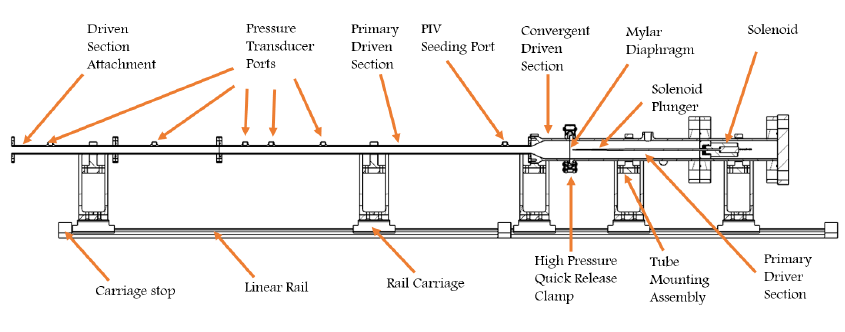
\includegraphics[width=1\textwidth]{fig9.PNG} 
	\caption{Shock tube facility schematic. Major parts of the
		system have been labelled.}
	\label{fig:shocktube}
\end{figure}	

The facility utilises compressed air delivered by the Monash University compressed air supply system. To produce a canonical transient supersonic jet a shock tube model is adopted \citep{john1962shock}. A typical shock tube consists of a high pressure section (driver section) and a low pressure section (driven section) separated by a diaphragm. Air enters the driver section until a desired pressure is reached, the diaphragm is then ruptured via a puncture from an actuated pin. Following the rupture, compression waves are fired down the driven section by the high pressure gas in the driver. As these compression waves travel down the tube they coalesce and form a shock wave that propagates into the test section, diffracts, and produces a transient supersonic jet. 

For the aims of this thesis, the supersonic transient jet will be studied with varied nozzle designs including a convergent, divergent and convergent-divergent configuration. Transient flow impingement will be tested via a flat plate set at $90^\circ$ to the flow. This impinging plate is set exactly at an angle of $90^\circ$ to the flow by a sequence of precisely $90^\circ$ connecting supports to the shock tube. The three nozzle designs and impingement plate will be integrated into the existing LTRAC Supersonic Jet Facility.

The relationship between the driver (4) pressure ratio and the ambient (1) pressure of the system is shown in Equation \ref{shock}, and was utilised to calculate the design incident Mach number propagating from the shock tube \citep{anderson2010fundamentals}. Figure \ref{fig:gas_relation} illustrates the effect of specific heat capacity ratio on the relation between incident Mach number and pressure ratio. Helium gas has increasingly lower pressure ratios for higher Mach numbers in comparison to air, and as a result was chosen as the driver section supply gas.

\begin{equation} \label{shock}
\frac{P_4}{P_1} = \frac{2\gamma_1M_1^2 - (\gamma_1 - 1)}{\gamma_1 + 1}\left(1 - \frac{\gamma_{4-1}}{\gamma_{1+1}}\frac{U_1}{U_4}\left(M_1 - \frac{1}{M_1}\right)\right)^{-2\gamma_4/\gamma_{4-1}}
\end{equation}
\smallskip
\begin{table}[H]
\centering
\caption{Experimental parameters.}
\label{tab:experiment}
\begin{tabular}{@{}ccc@{}}
\toprule
\toprule
\textbf{Component} & \textbf{Nomenclature} & \textbf{Value} \\ \midrule
\multicolumn{3}{c}{Shock Tube}                                  \\ \midrule
Driver section     & $X_{driver}$          & ??                 \\
Driven section     & $X_{driven}$          & ??                 \\ \midrule
\multicolumn{3}{c}{Converging Nozzle}                           \\ \midrule
Entry diameter     & $D_i$                 & 12.5 mm            \\
Exit diameter      & $D_f$                 & 6.2 mm             \\
Exterior angle     & $\theta$              & $60^\circ$         \\ \midrule
\multicolumn{3}{c}{Diverging Nozzle}                            \\ \midrule
Entry diameter     & $D_i$                 & 12.5 mm            \\
Exit diameter      & $D_f$                 & 18.7 mm            \\
Exterior angle     & $\theta$              & $60^\circ$         \\ \midrule
\multicolumn{3}{c}{Converging-diverging Nozzle}                 \\ \midrule
Entry diameter     & $D_i$                 & 12.5 mm            \\
Throat diameter    & $D_t$                 & 6.4 mm             \\
Exit diameter      & $D_f$                 & 18.7 mm            \\
Exterior angle     & $\theta$              & $60^\circ$         \\ \midrule
\multicolumn{3}{c}{Impingement Plate}                           \\ \midrule
Base               & $B_p$                 & 110 mm             \\
Height             & $H_p$                 & 200 mm             \\
Thickness          & $T_p$                 & 10 mm              \\ \bottomrule
\bottomrule
\end{tabular}
\end{table}

\begin{figure}[H] 
	\centering
	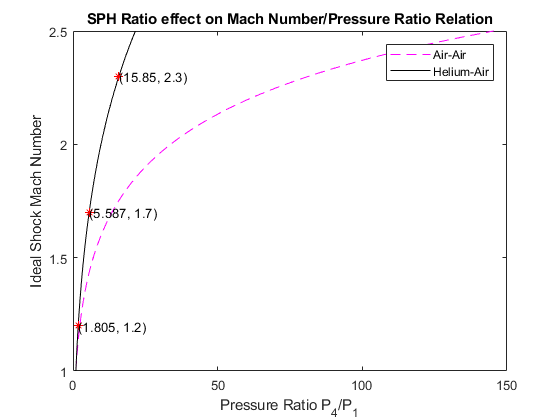
\includegraphics[scale=0.9]{fig1.png} 
	\caption{Specific Heat Capacity Ratio effect on Mach Number/Pressure Ratio Relation.}
	\label{fig:gas_relation}
\end{figure}

\subsection{Schlieren Imaging}
Schlieren imaging is a visualization technique that utilises the refraction of light to produce focused optical images of transparent media. Point source light is collimated and passed through a test region containing a transparent media with inhomogeneities. Light entering the test region will refract at varied degrees according to an inhomogeneous density distribution present. When refraction occurs the curvature $\epsilon$ of light, for a given test section length L, and refractive index $n_0$ can be calculated using Equations \ref{eqn:curv_x} and \ref{eqn:curv_y} for x and y orthogonal coordinates. The light is then refocused and a knife-edge is used to partially block a fraction of incident light from the screen or camera.

\begin{equation}\label{eqn:curv_x}
\epsilon_x = \frac{L}{n_0}\frac{\delta n}{\delta x}
\end{equation}

\begin{equation}\label{eqn:curv_y}
\epsilon_y = \frac{L}{n_0}\frac{\delta n}{\delta y}
\end{equation}

The shock-driven, transient, supersonic jet is measured using a Toepler Z-type schlieren apparatus \citep{settles2001schlieren} (illustrated in Figure \ref{fig:schlieren}). This Z-type apparatus incorporates parabolic mirrors to collimate the light. Parabolic mirrors eliminates problems associated with chromatic aberration and provides a unique advantage for imaging in comparison to systems using lenses. However, the use of mirrors introduces common imaging problems including coma and astigmatism. Coma is the result of off-axis, incorrect parabolic mirror tilting and disrupts the collimated light beam. It also causes the focal point of the parabolic mirrors to spread into a line. This issue is resolved by careful calibration of each parabolic mirror titling to achieve an overall cancelling effect.  Astigmatism is similarly caused by tilting the parabolic mirror off-axis. It occurs due alternating path lengths of light dependent on their respective optical plane. Astigmatism results in different focal points for each plane of propagating light and requires the knife-edge to be positioned for different density gradients. For Z-type schlieren configurations, coma and astigmatism is minimised by restricting the offset angle (tilt) of the parabolic mirrors to minimum achievable values. Careful calibration prior to experimentation is required to avoid problems associated with coma and astigmatism. This involves correcting mirror allingments, adjusting the knife edge, and positioning the camera distance until the desired image is displayed. The parabolic mirrors used in the facility have an an effective focal length of $1200mm$ and the light source was supplied by a pulsed LED \citep{willert2012assessment}. 

\begin{figure}[H] 
	\centering
	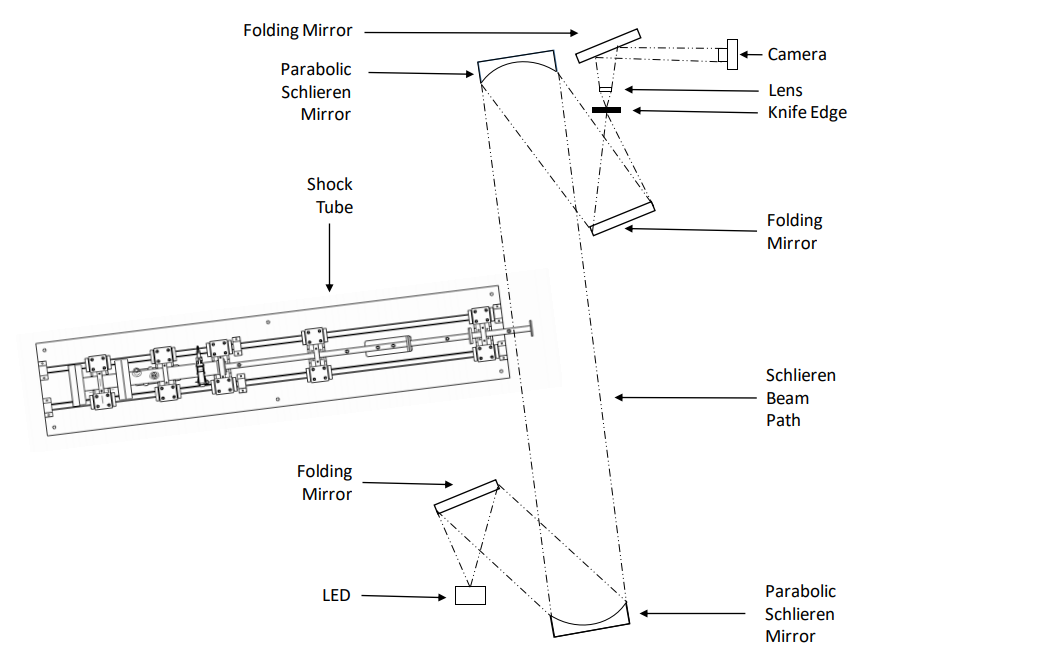
\includegraphics[width=1\textwidth]{schlieren.png} 
	\caption{Detailed schlieren system diagram.}
	\label{fig:schlieren}
\end{figure}

\subsubsection{High Resolution Imaging}
High spatial-resolution images were captured using the Chronos camera with a resolution
of 1280x1024 pixels at 1057 frames per second (fps). Image sets varied in
size and were determined by the fluid dynamic structures captured. If a set contained significant detail of the transient process by nature it was larger. Smaller sets were recorded if the respective trailing jet displayed unique flow qualities. Image sets containing information on the transient process were of more significance given the aims of this thesis and were a priority for capturing, this led to the implementation of high speed cameras. The schlieren parameters for several conditions using the Chronos camera are included in Table \ref{tab:highres}, Figure \ref{fig:settle} shows the physical representation of each parameter.

\subsubsection{High Speed Imaging}
High speed images were captured using the Shimadzu HPV-1 camera with a resolution of 312 x 260 pixels and a frame rate of up to 1 million fps. Image sets were approximately constant give this camera was utilised to specifically capture the transient supersonic jet. Image quality provided by the Shimadzu HPV-1 is low in comparison to the Chronos camera. As a result, data from the Shimadzu was solely used for flow analysis and not flow feature discussions. The schlieren parameters for several conditions using the Shimadzu HPV-1 camera are included in Table \ref{tab:highspeed}, Figure \ref{fig:settle} shows the physical representation of each parameter.

\begin{table}[h]
\centering
\caption{High spatial-resolution schlieren parameters.}
\label{tab:highres}
\begin{tabular}{@{}lllll@{}}
\toprule
b (mm) & h (mm) & Magnitude & $f_3$ (mm) & e (mm)  \\ \midrule
50     & 20     & 0.169     & 204.911   & 201.448 \\
35     & 15     & 0.241     & 294.902   & 287.782 \\
20     & 10     & 0.422     & 525.836   & 503.620 \\
12     & 6      & 0.704     & 902.949   & 839.366 \\ \bottomrule
\end{tabular}
\end{table}

\begin{table}[h]
\centering
\caption{High speed schlieren parameters.}
\label{tab:highspeed}
\begin{tabular}{@{}lllll@{}}
\toprule
b (mm) & h (mm) & Magnitude & $f_3$ (mm) & e (mm)   \\ \midrule
50     & 20     & 0.721     & 926.821    & 859.956  \\
35     & 15     & 1.031     & 1369.672   & 1228.509 \\
20     & 10     & 1.803     & 2622.970   & 2149.891 \\
12     & 6      & 3.006     & 5123.180   & 3583.152 \\ \bottomrule
\end{tabular}
\end{table}

\begin{figure}[H] 
	\centering
	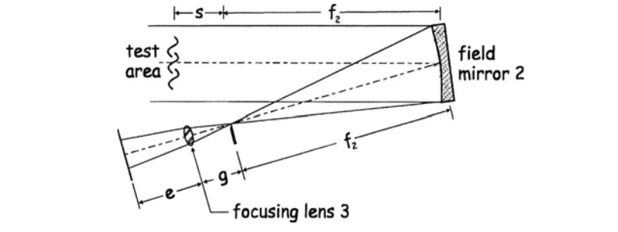
\includegraphics[scale=0.8]{settle.png} 
	\caption{Schlieren parameters \citep{settles2001schlieren}.}
	\label{fig:settle}
\end{figure}

\subsubsection{Limitations}
Schlieren imaging has a number of limitations. Firstly, schlieren images are constructed using density gradients within the test region. The gradients are integrated over the optical path and as a result, images are developed as two-dimensional projections of an original three-dimensional fluid flow. This introduces possible incorrect projects of three-dimensional features. Additionally, the technique is line-of-sight dependent as the light must be collimated and refocused in order to produce an image. This restricts the layout of test section and sets requirements on the amount of space required for the apparatus. 

\subsection{Facility Development and Calibration}
\subsubsection{Nozzle Design}
A convergent, divergent, and convergent-divergent nozzle was designed using CAD and manufactured by the Engineering department Mechanical Workshop. All three nozzle designs adopt geometry ratios implemented in the nozzles designed by Technical University of Berlin (TUB). To prevent reflecting flow and acoustic feedback loop interference, each nozzle geometry was designed with a $60^\circ$ exterior angle and a $0.5mm$ lip \citep{poldervaart1968photographic}. Each nozzle design and subsequently manufactured component is shown in Figures \ref{fig:con_noz}, \ref{fig:div_noz}, and \ref{fig:con_div_noz} below. 
 
\begin{figure}[!tbh]
  \centering
  \subfloat[CAD design (all measurements are in mm).]{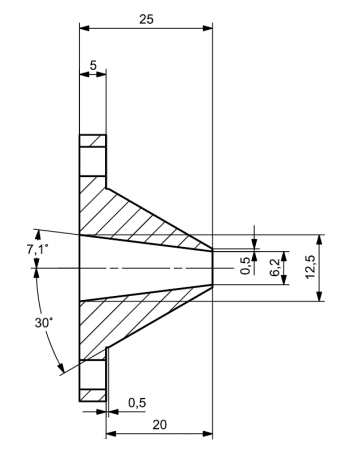
\includegraphics[width=0.4\textwidth]{convergent_cad.png}}
  \hfill
  \subfloat[Manufactured nozzle.]{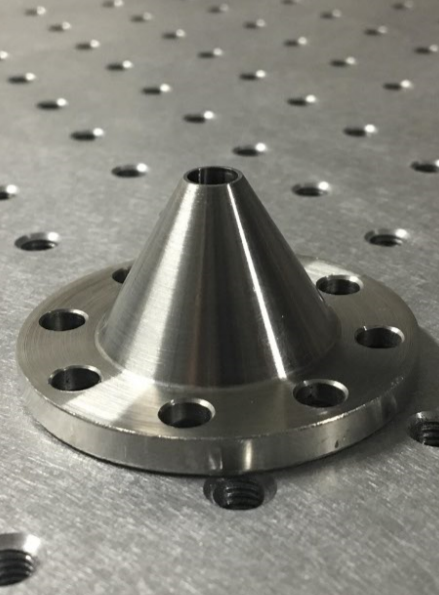
\includegraphics[width=0.4\textwidth]{con_noz.png}}
  \caption{Convergent nozzle.}
  \label{fig:con_noz}
\end{figure}

\begin{figure}[!tbh]
  \centering
  \subfloat[CAD design (all measurements are in mm).]{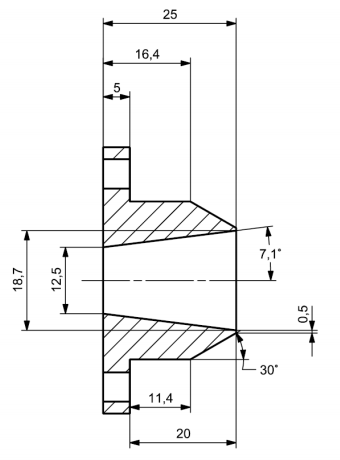
\includegraphics[width=0.4\textwidth]{divergent_cad.png}}
  \hfill
  \subfloat[Manufactured nozzle.]{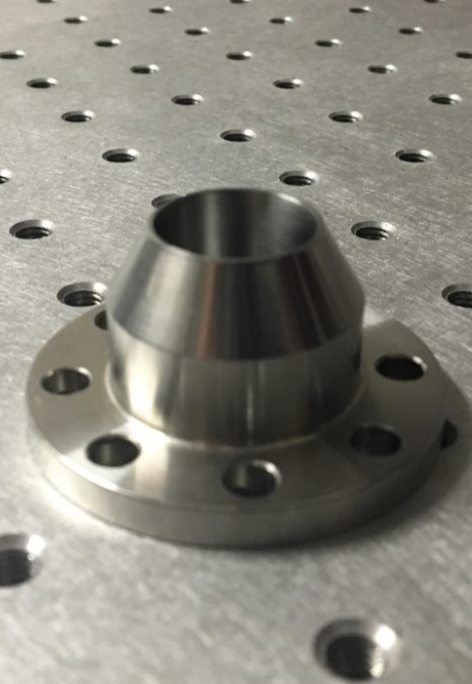
\includegraphics[width=0.4\textwidth]{div_noz.png}}
  \caption{Divergent nozzle.}
  \label{fig:div_noz}
\end{figure}

\begin{figure}[!tbh]
  \centering
  \subfloat[CAD design (all measurements are in mm).]{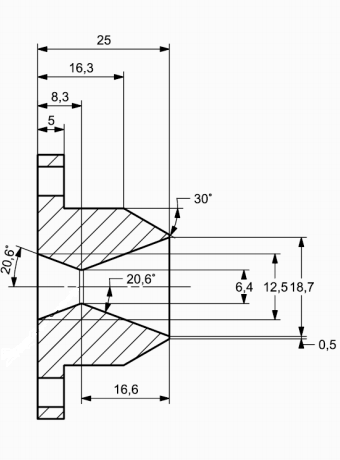
\includegraphics[width=0.4\textwidth]{con_div_cad.png}}
  \hfill
  \subfloat[Manufactured nozzle.]{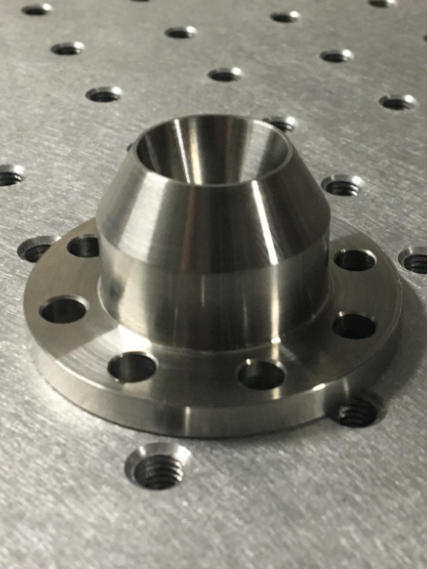
\includegraphics[width=0.4\textwidth]{con_div_noz.png}}
  \caption{Convergent-divergent nozzle.}
  \label{fig:con_div_noz}
\end{figure}

\subsubsection{Impingement Plate Design}
The impingement plate as shown in Figure \ref{fig:plate_draw} is constructed such that it is $90^{\circ}$ to the direction of the flow, and will appear infinite in the reference frame of the oncoming flow. The plate is mounted on rails which fix to the shock tube rig, this construction can be adjusted to 1 and 4 inner diameters. This construction allows the plate to be removed and replaced with another plate of alternate geometry for future research. During the evolution of a transient supersonic jet, the vortex is fully formed at approximately 3 inner diameters from the exit for a conventional, no nozzle, shock tube \citep{mariani2013head}. As a result, an impingement plate distance is chosen below and above this limit at 1 and 4 inner diameters, respectively. 

\begin{figure}[!tbh] 
	\centering
	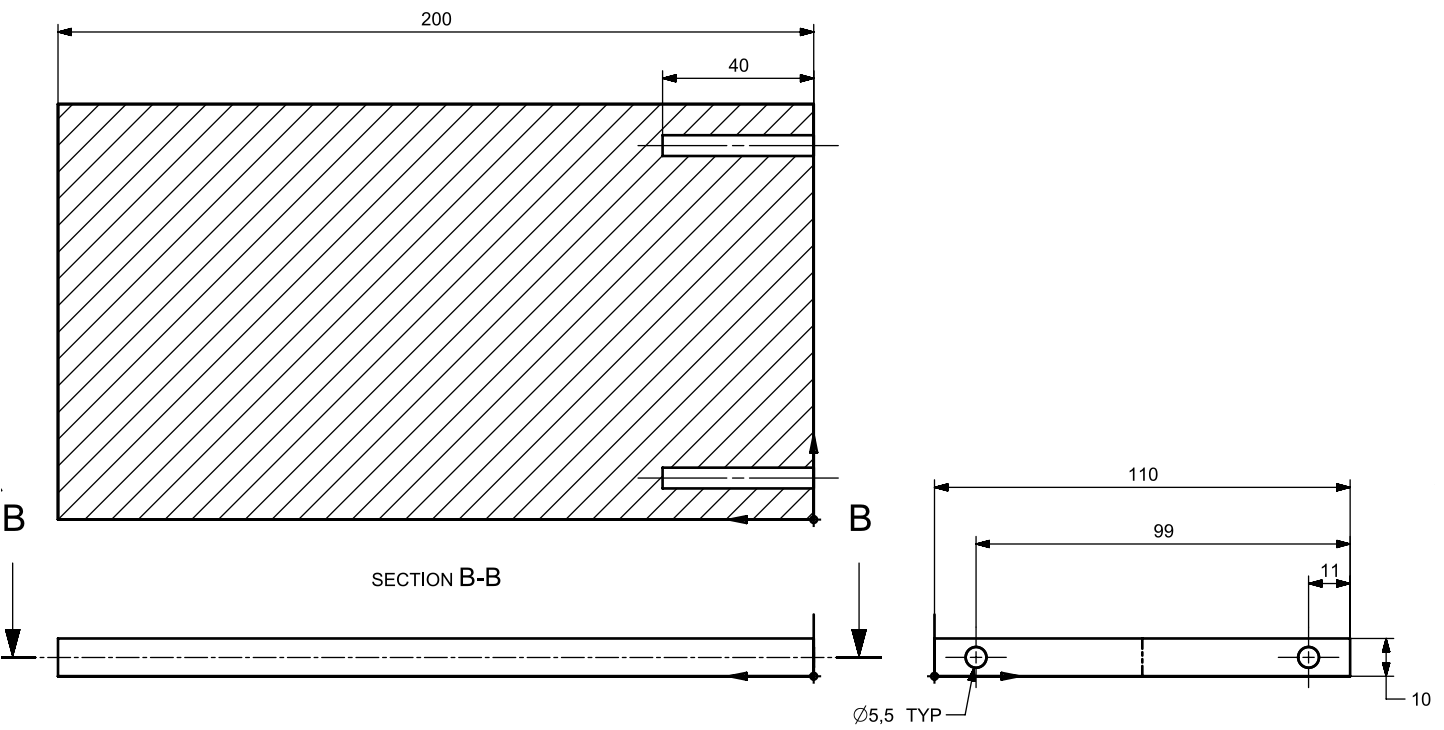
\includegraphics[width=1\textwidth]{plate_draw.png} 
	\caption{Impingement plate CAD design (all measurements are in mm).}
	\label{fig:plate_draw}
\end{figure}


\subsubsection{Impingement Plate Development}
The first iterative design of the plate resulted in a significant unexpected wobble during jet impingement. Figures \ref{fig:wobble_iter1}, \ref{fig:wobble_iter2}, and \ref{fig:wobble} are constructed using post processing techniques detailed in Section \ref{sect:post}, and illustrates the pixel displacement of the plate resulting from flow impingement for design iterations 1, 2, and 3 respectively. Figure \ref{fig:wobble_iter1} illustrates the first design iteration which involved the incorrect tightening of impingement plate bolt fixings. This caused an oscillatory pixel displacement response as a result of the significant freedom of movement given to the plate by inadequate fastening. The pixel displacement decreases as a function of increasing frame number, this is governed by the initial transient supersonic jet impingement, underexpanded trailing jet impingement, and the decreasing back pressure of the shock tube. Figures \ref{fig:wobble_iter2} and \ref{fig:wobble} represent the pixel displacement for an adequately fastened impinging plate and a reinforced impinging plate structure. Both figures highlight the evolution of the transient supersonic jet. Initially at frame 0 the pixel displacement is similarly 0 given impingement has not yet occurred. The sudden jump in pixel displacement in frame 1, and subsequent pixel displacement in the following frames represents the impingement of the evolving transient supersonic jet. As the supersonic jet becomes an underexpanded trailing jet the relative pressure of the flow on the plate decreases as the back pressure in the shock tube decreases. Given the limitations of the recording time for the Chronos camera, the full evolution of the underexpanded trailing jet was not captured and as a result, the pixel displacement shown in Figure's \ref{fig:wobble_iter1}, \ref{fig:wobble_iter2}, and \ref{fig:wobble} have final values not representative of pixel displacement at the end of the underexpanded jet process, and once the back pressure in the shock tube is approximately equal to atmospheric pressure. If the full fluid dynamics process was captured it is to be expected that the pixel displacement once the back pressure within the shock tube reaches atmospheric pressure, or once the pressure induced on impinging plate is negligible would be 0. This design error was addressed between iterations 2 and 3 (Figures \ref{fig:wobble_iter2} and \ref{fig:wobble}) with the addition of support brackets as shown in Figure \ref{fig:plate_iter}. The position of the support brackets was chosen such that interference with the transient supersonic jet and impingement by-products was not possible. This design change had little affect on the pixel displacement of the impingement plate. In comparison to Figure \ref{fig:wobble_iter2}, Figure \ref{fig:wobble} contains a lower magnitude minima pixel displacement value although, the range between maxima and minima stays approximately the same for both iterations. This suggests the design of the impinging plate needs further modification with additional supports and improved fastening bolts. However, in Figures \ref{fig:wobble_iter2} and \ref{fig:wobble} the largest pixel displacement approximates to $0.6\%$ and for the purposes of this thesis will be considered negligible.

\begin{figure}[H]
  \centering
  \subfloat[Iteration 2.]{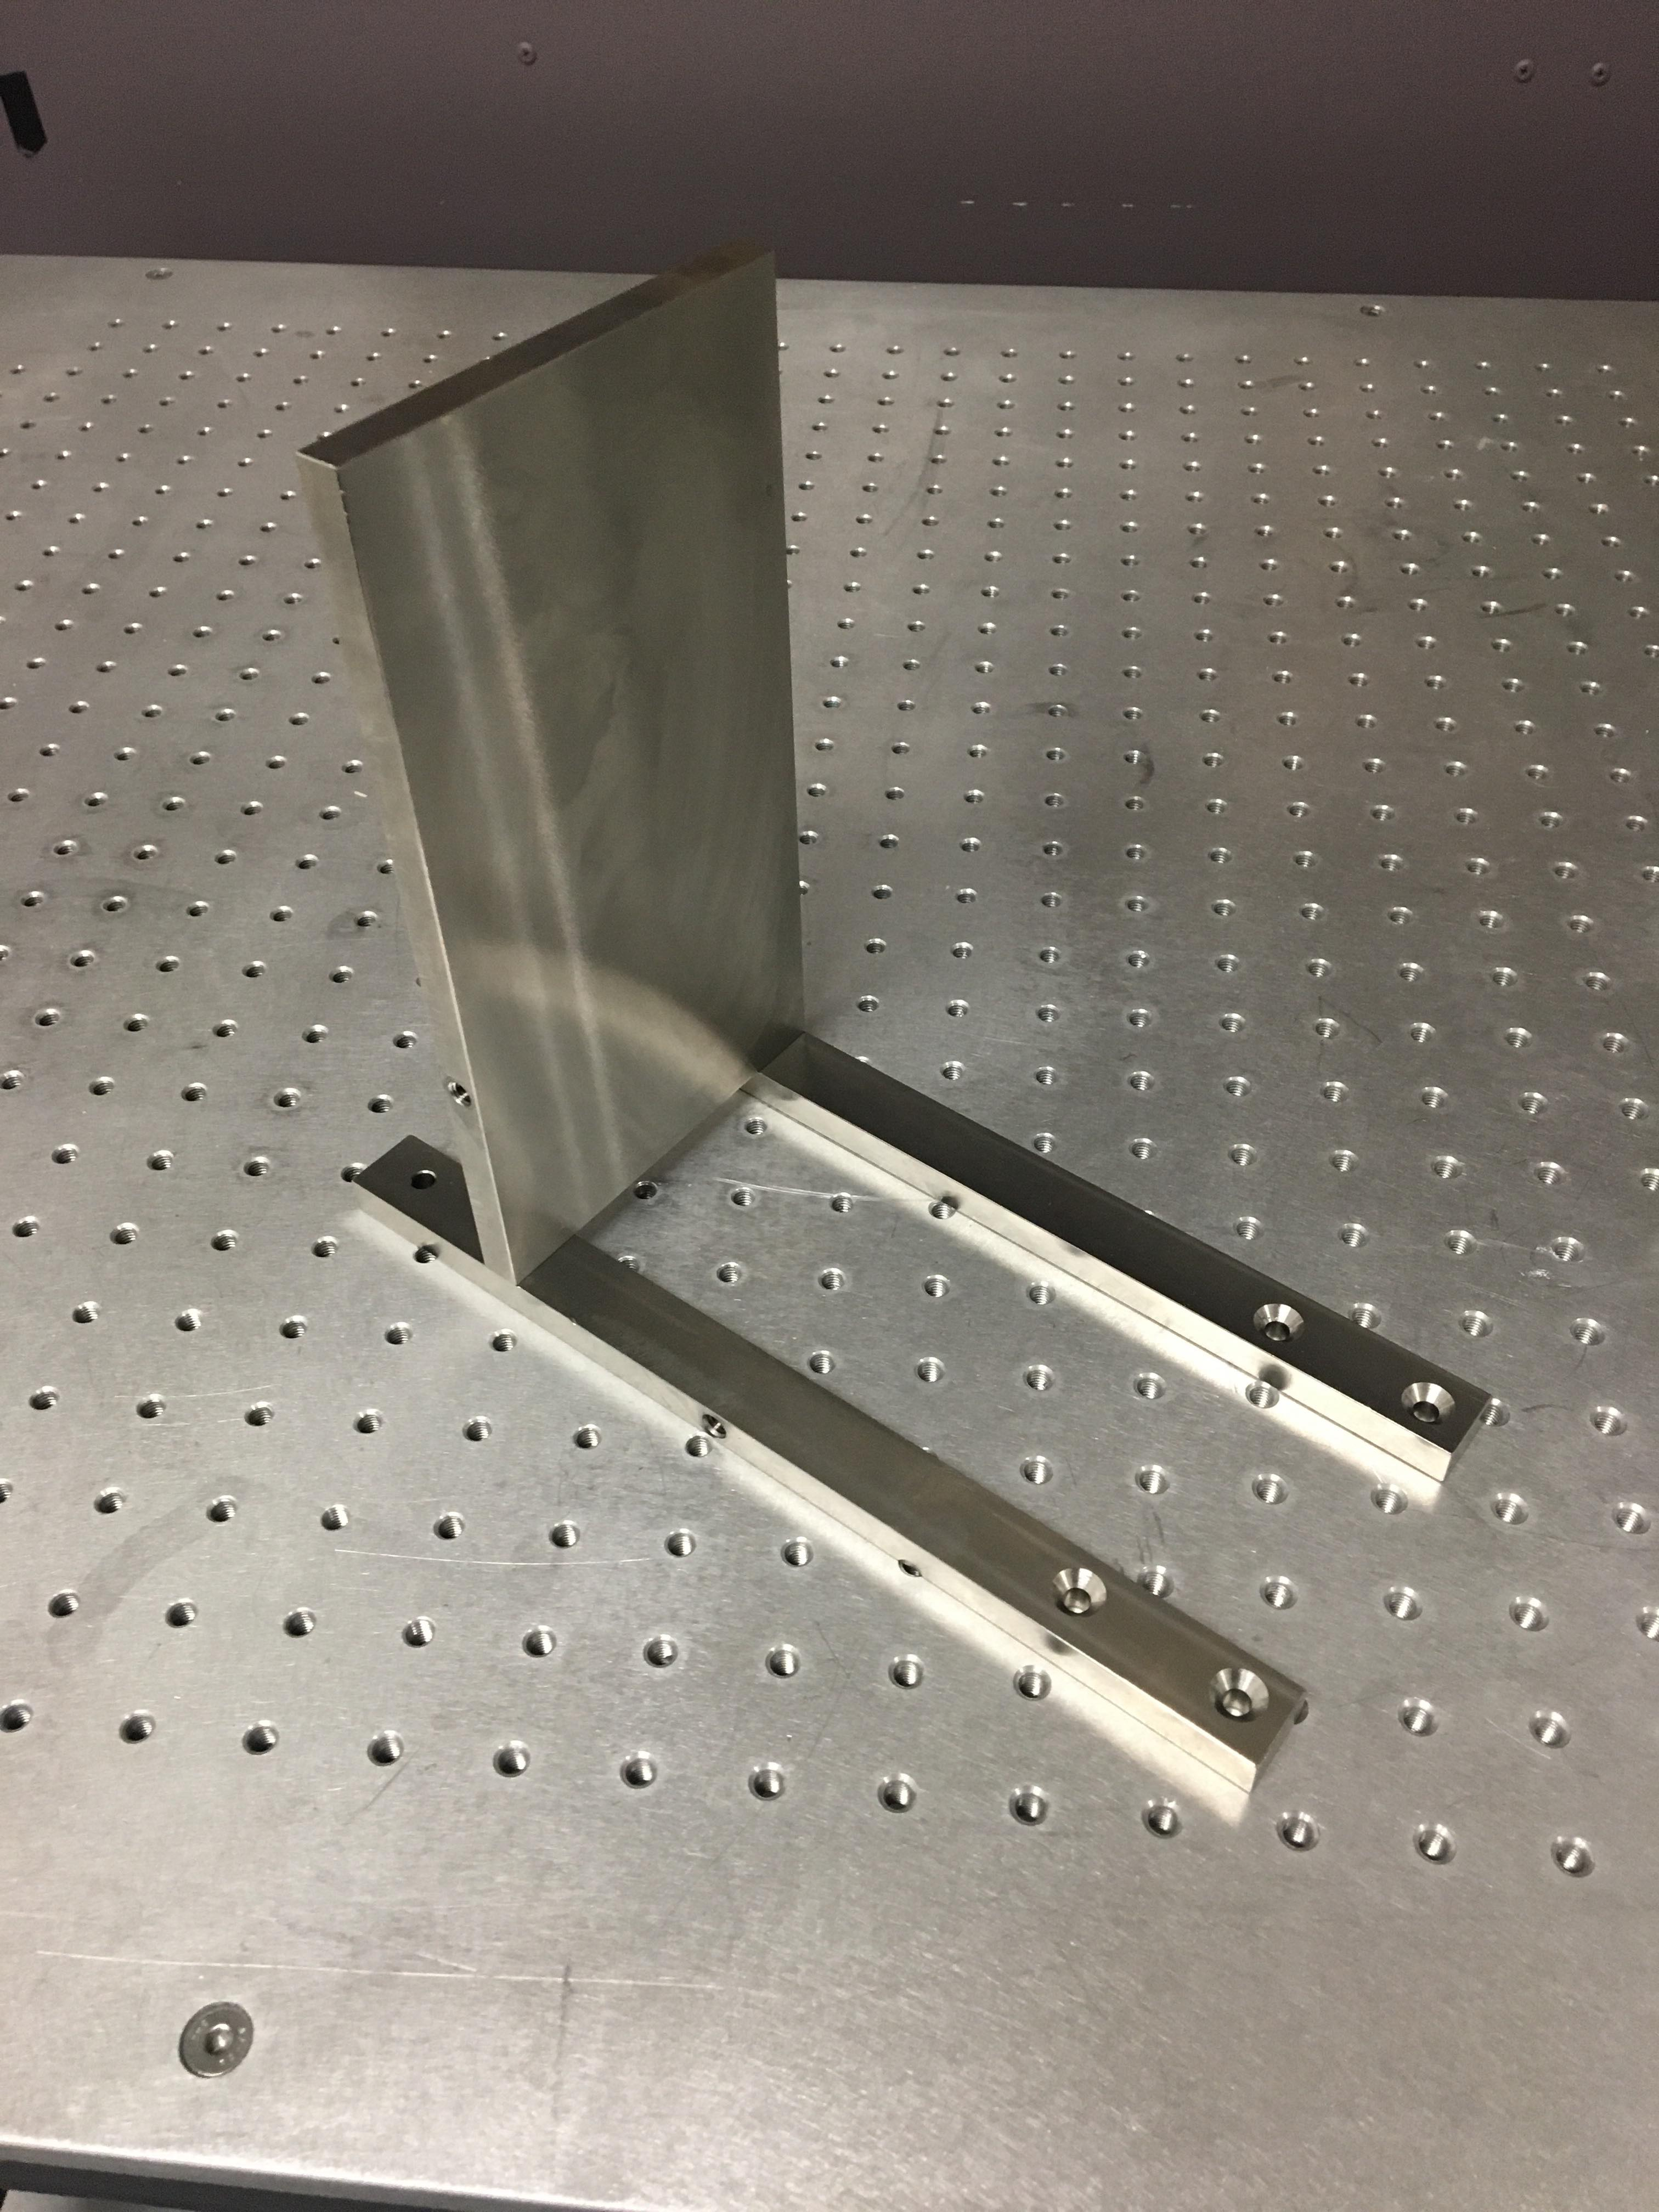
\includegraphics[width=0.4\textwidth]{iter1.jpg}}
  \hfill
  \subfloat[Iteration 3.]{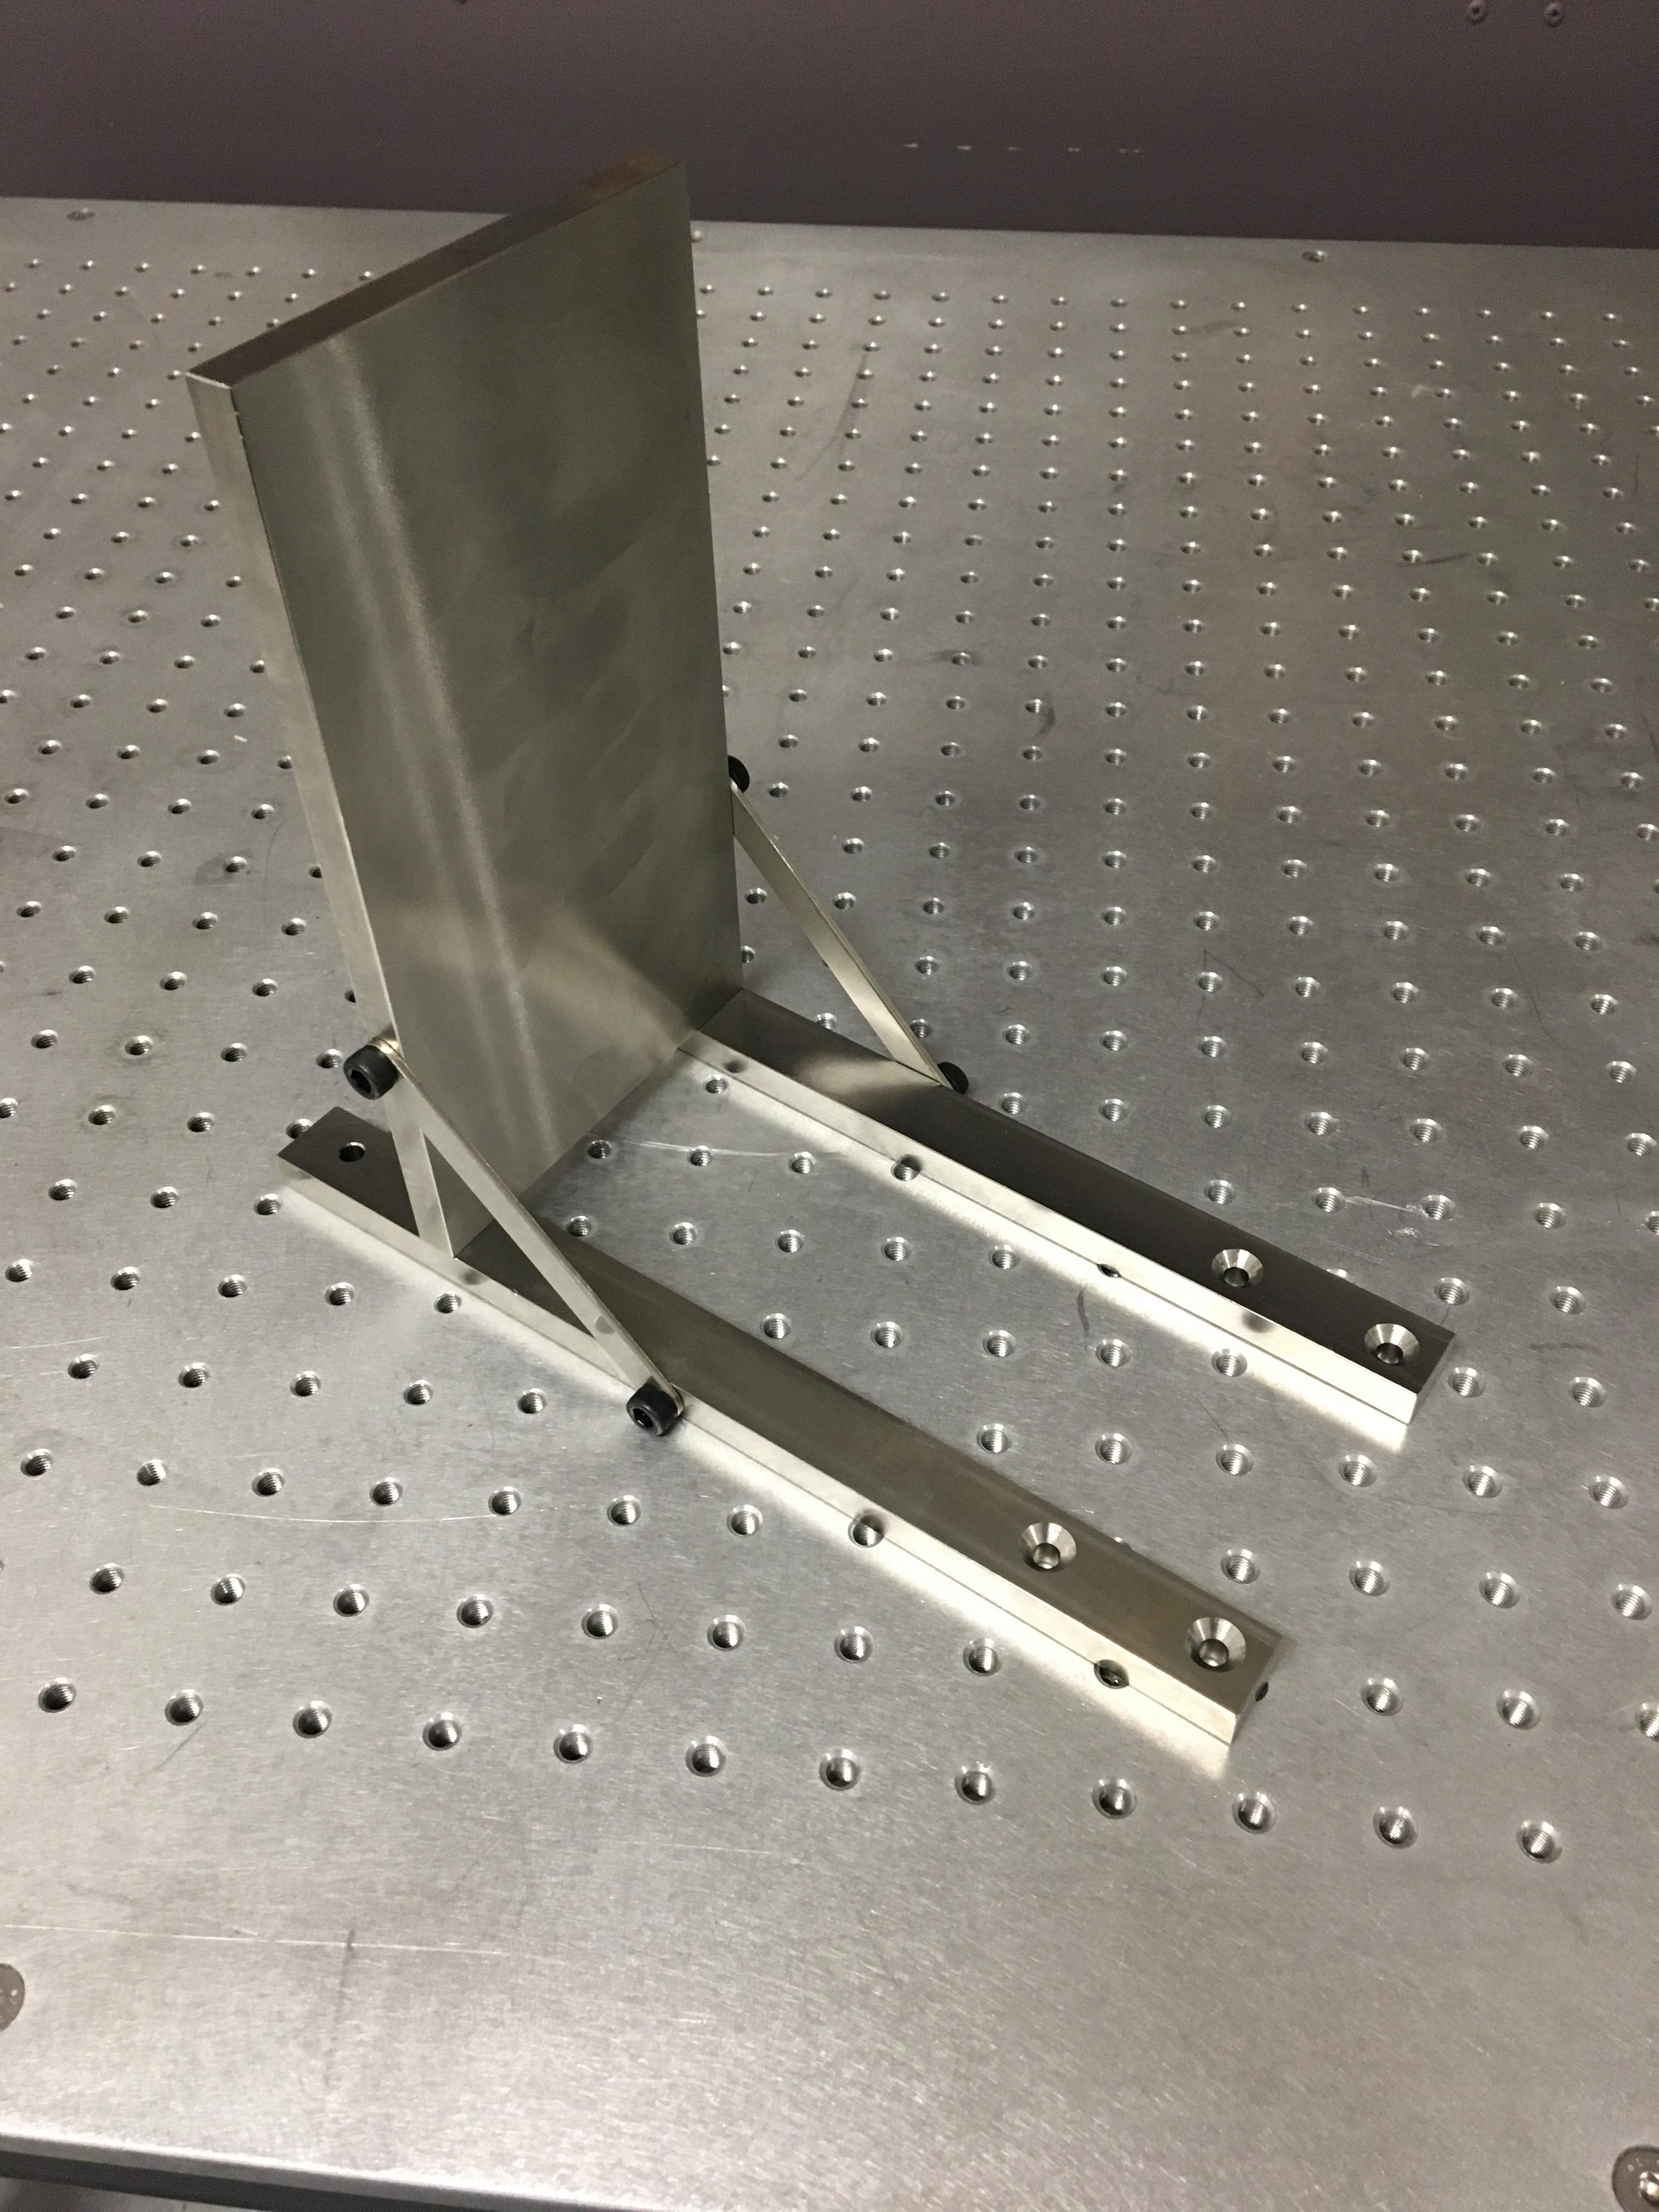
\includegraphics[width=0.4\textwidth]{iter2.jpg}}
  \caption{Impinging plate design iterations.}
  \label{fig:plate_iter}
\end{figure}

\begin{figure}[H] 
	\centering
	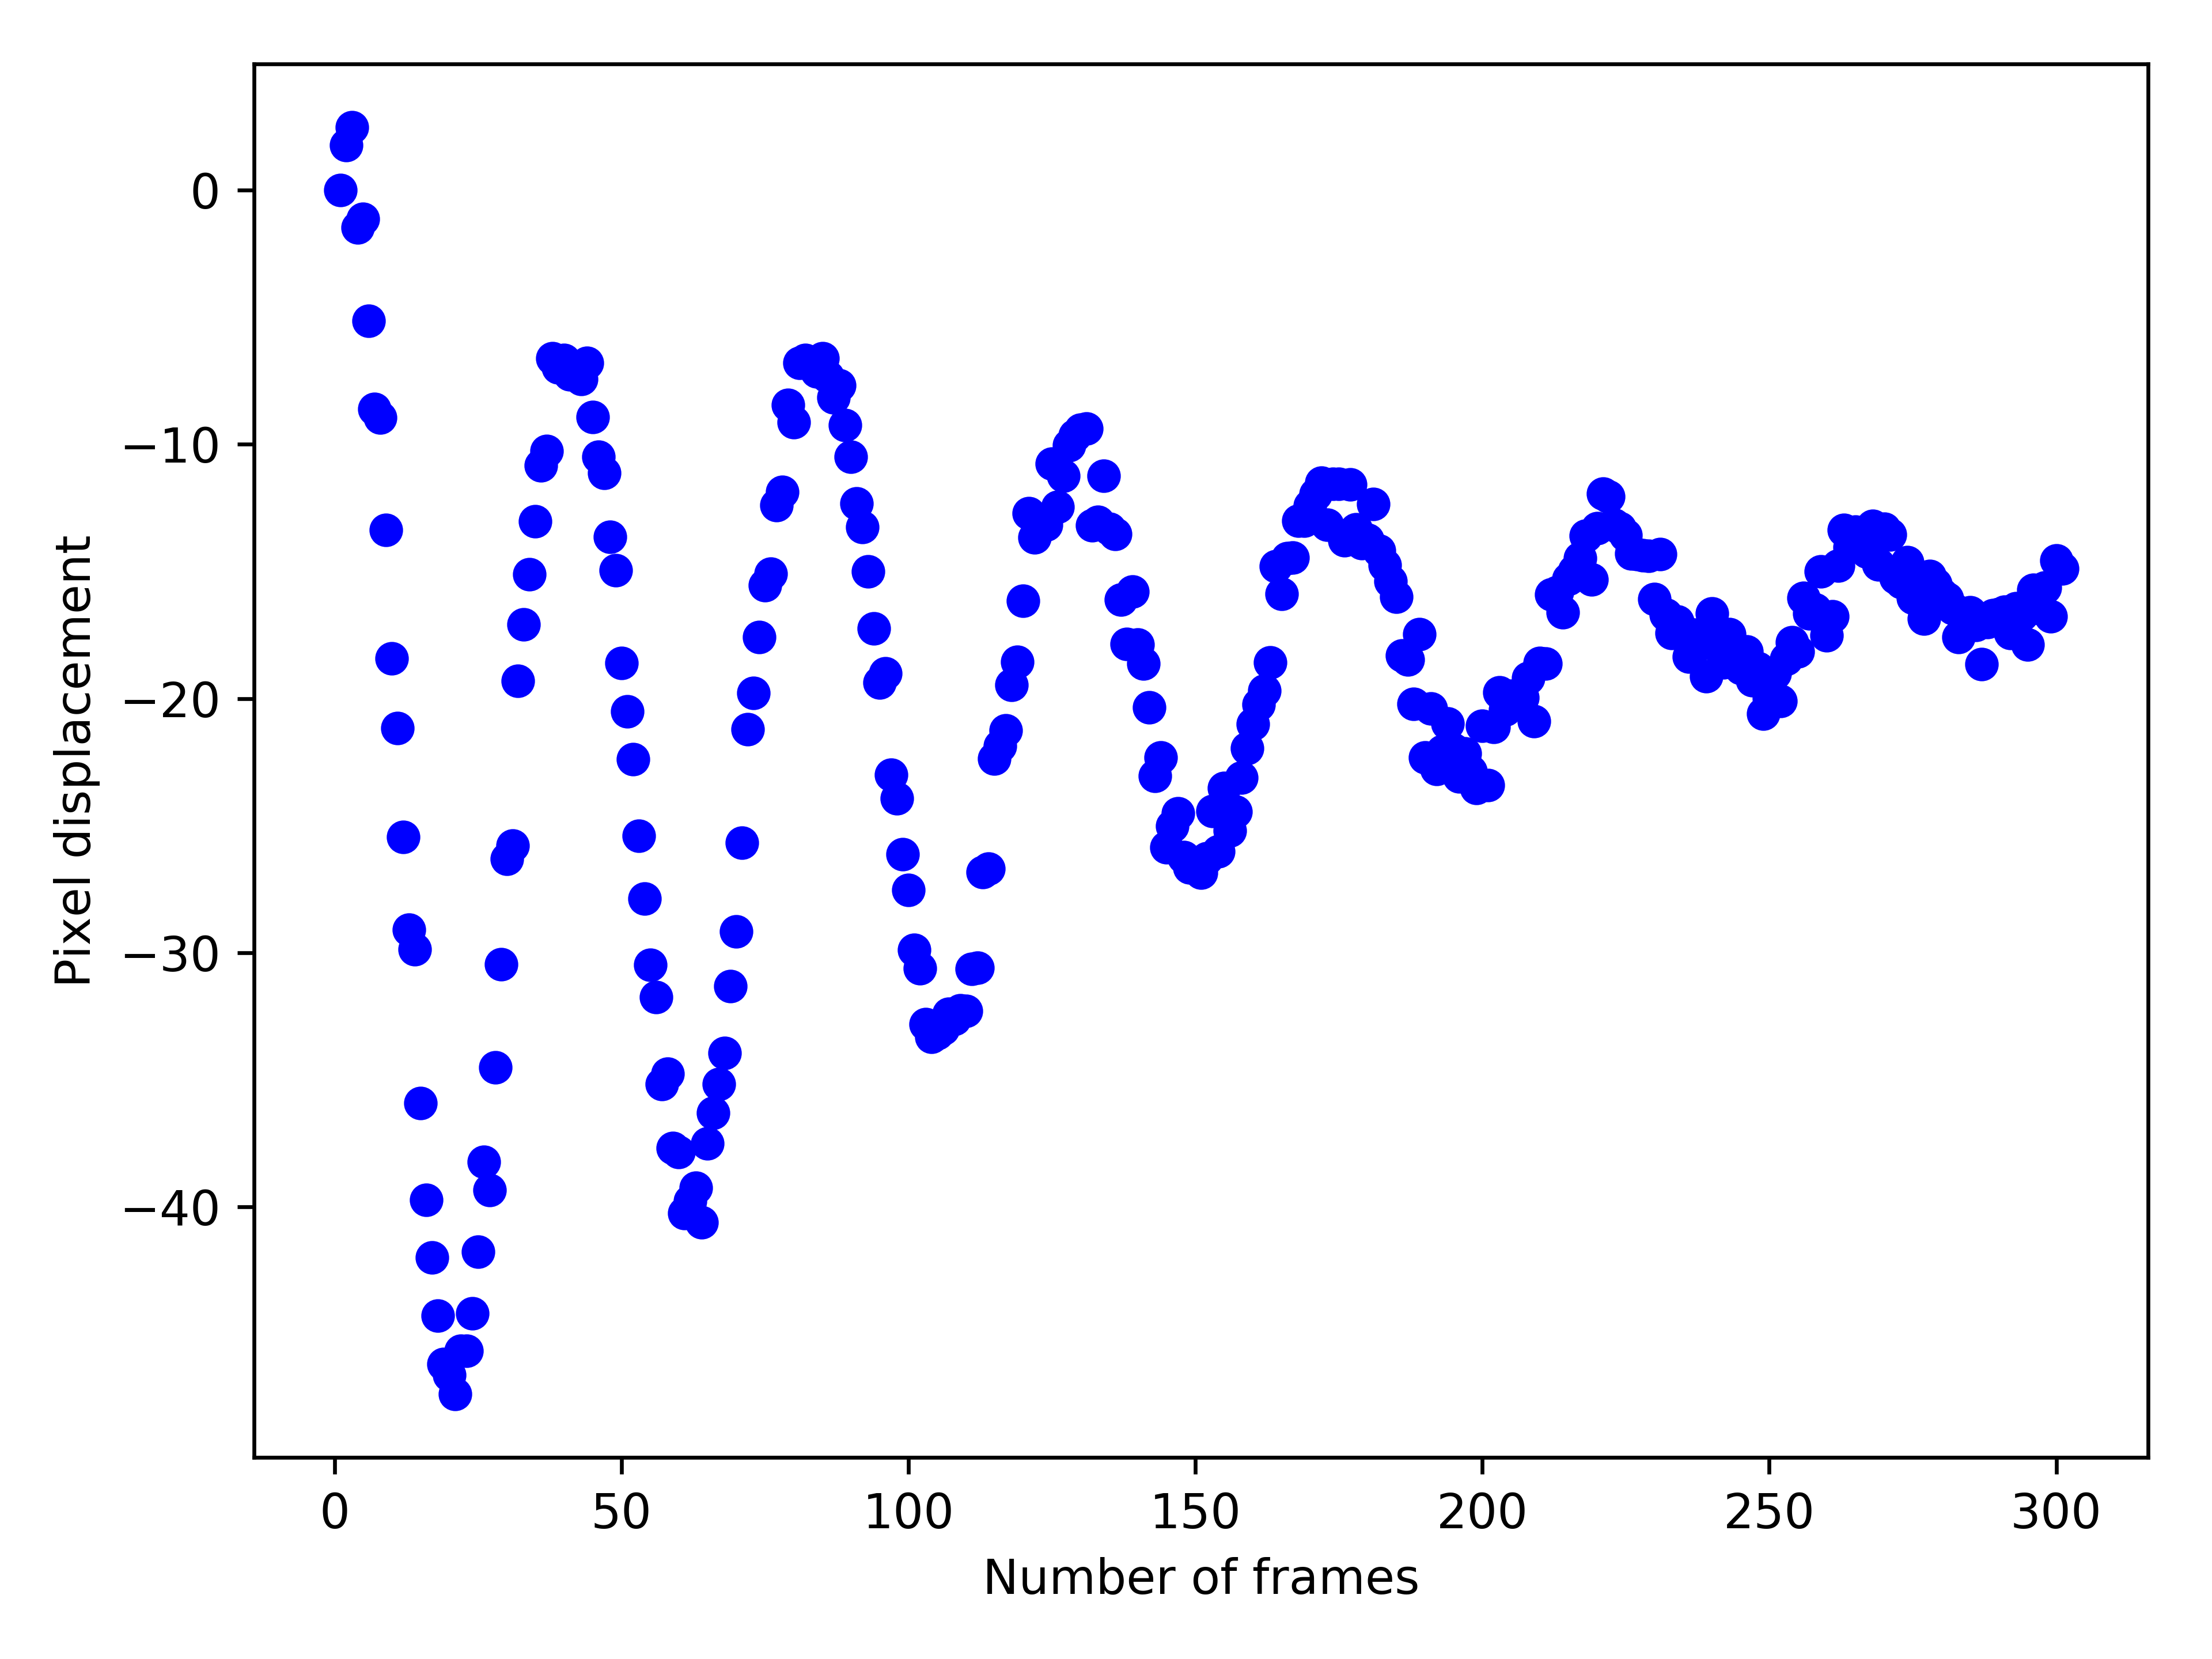
\includegraphics[width=0.88\textwidth]{wobble_iter1.png} 
	\caption{Plate displacement for design iteration 1.}
	\label{fig:wobble_iter1}
\end{figure}

\begin{figure}[H] 
	\centering
	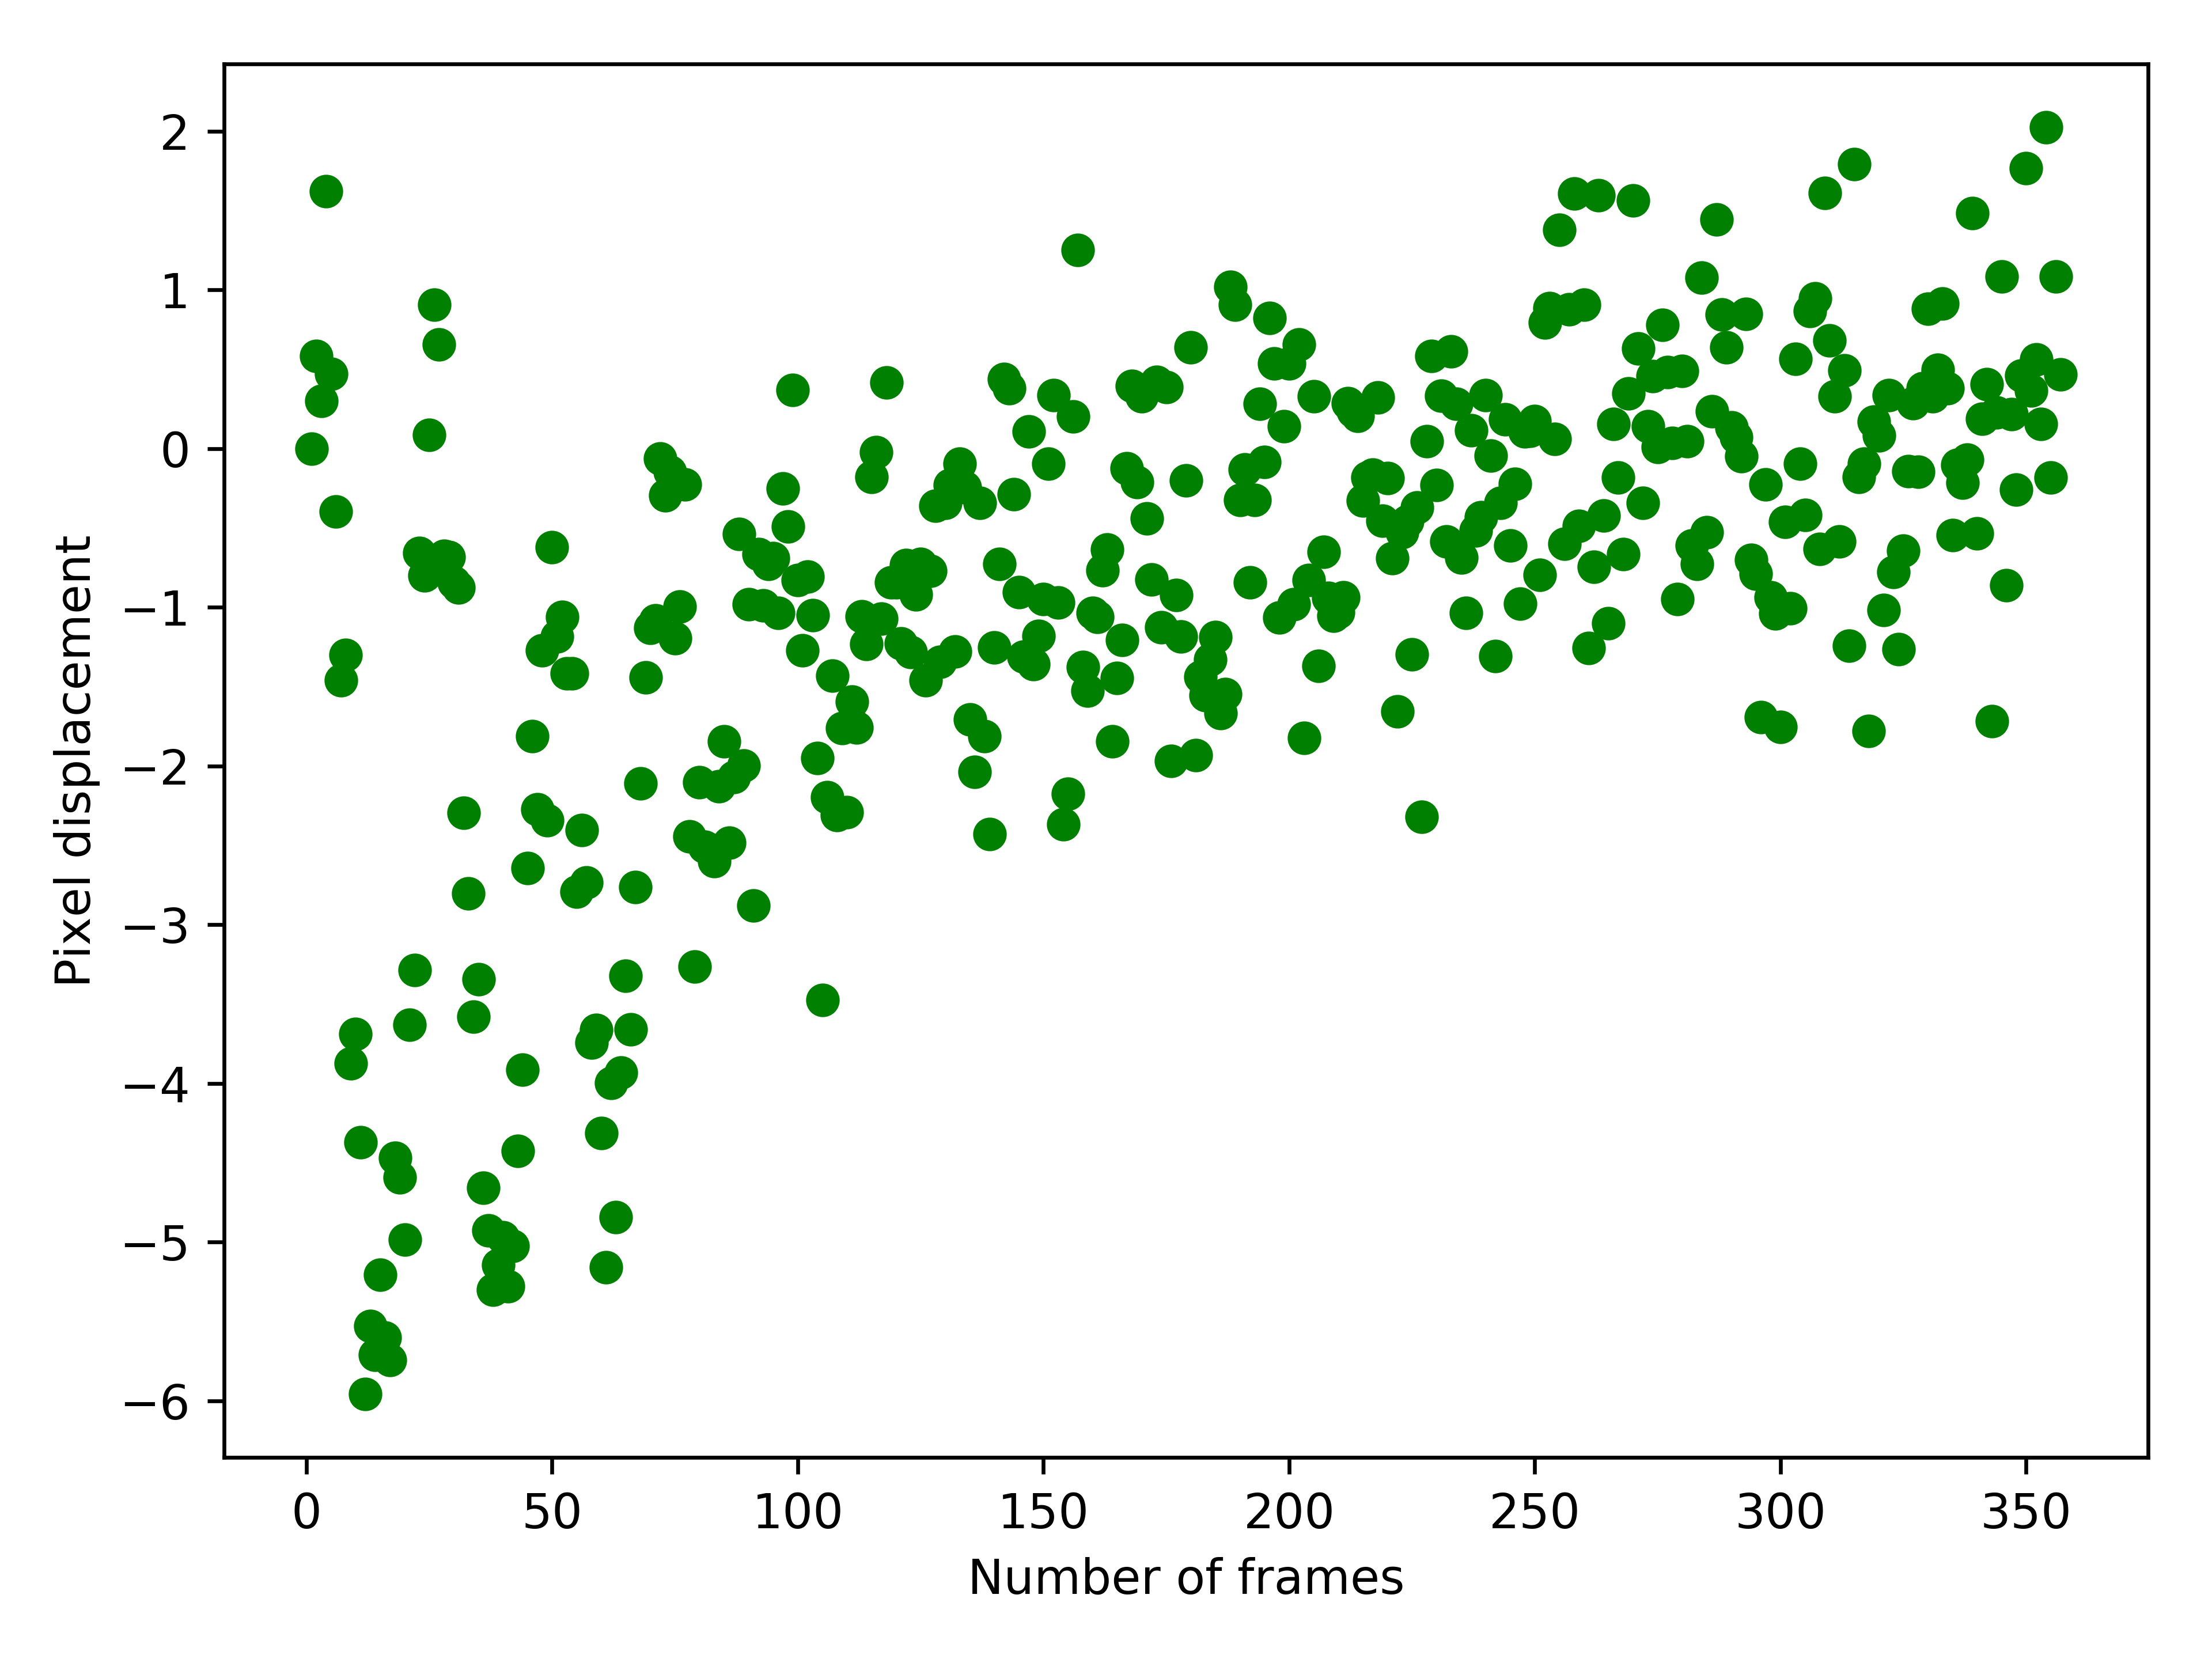
\includegraphics[width=0.88\textwidth]{wobble_iter2.png} 
	\caption{Plate displacement for design iteration 2.}
	\label{fig:wobble_iter2}
\end{figure}

\begin{figure}[H] 
	\centering
	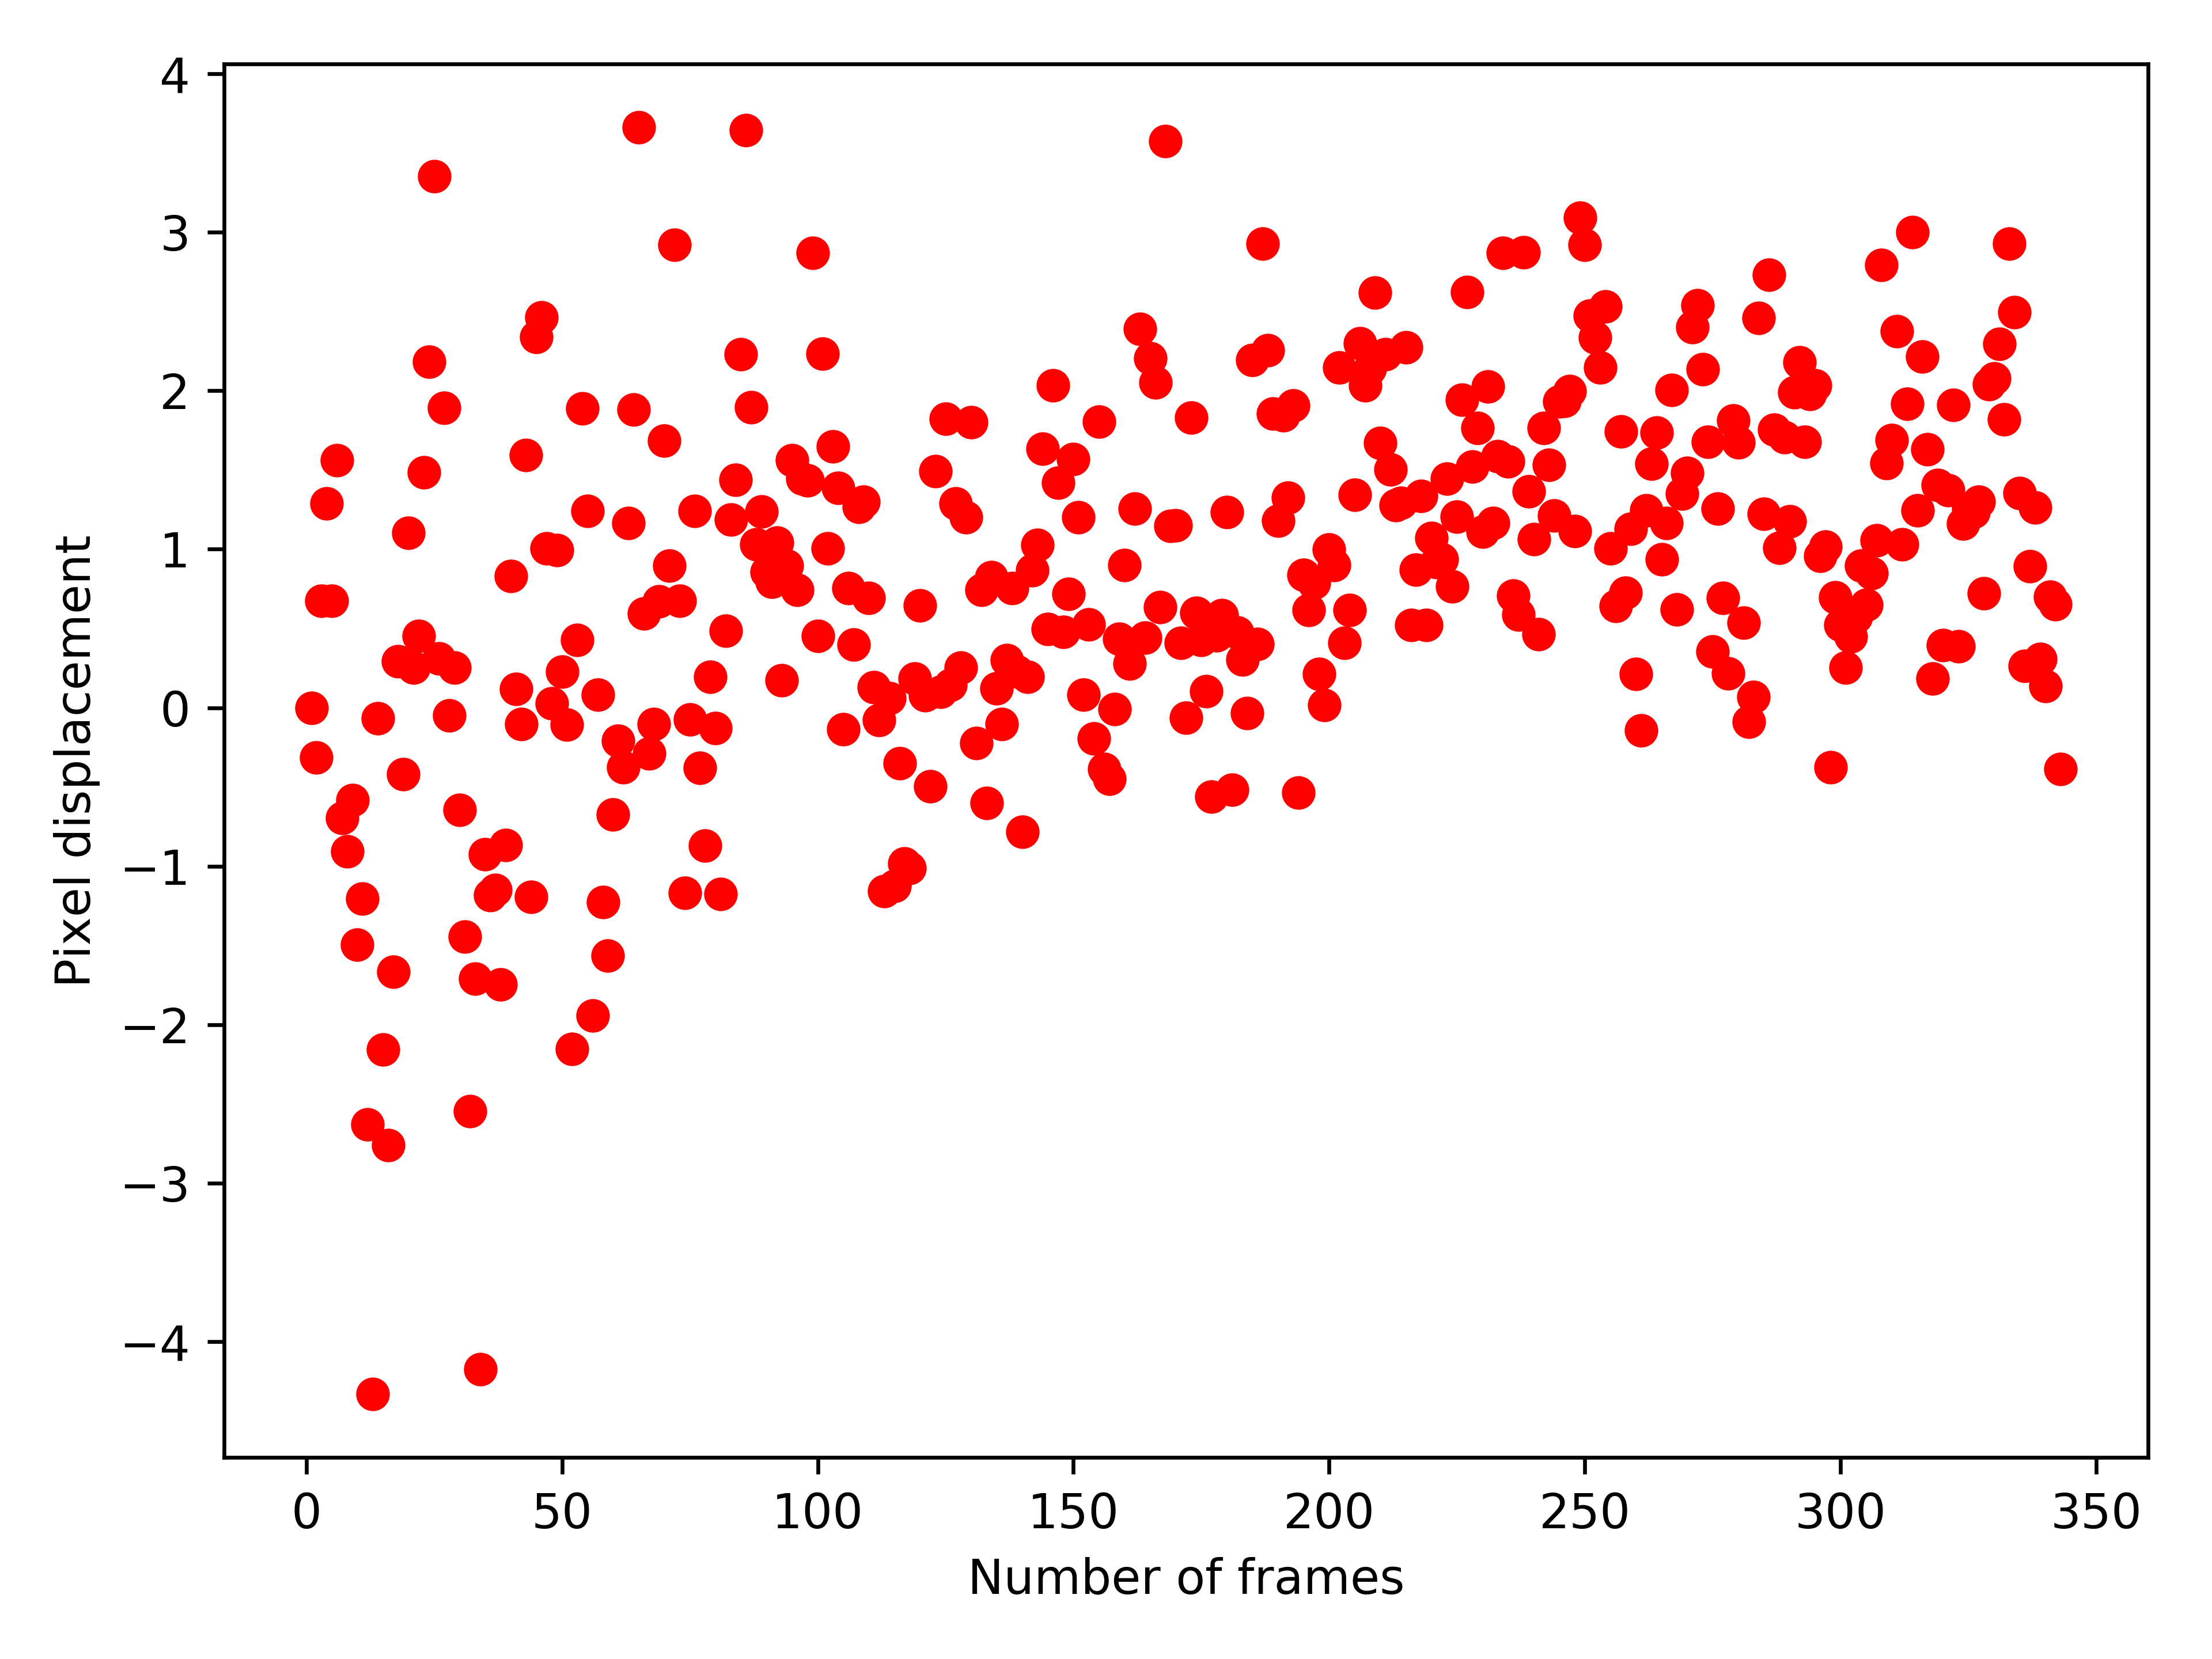
\includegraphics[width=0.88\textwidth]{wobble.png} 
	\caption{Plate displacement for design iteration 3.}
	\label{fig:wobble}
\end{figure}

\subsubsection{Hydrostatic Test}

A hydrostatic test is required of all apparatuses operating under pressurised conditions. The testing of the shock tube driver section involved sealing all non operational valves and pressurising the driver section with water until failure. An air outlet was initially left open and sealed once the driver section was completely filled with water. Figure \ref{fig:hydro_test} illustrates the testing configuration used and Table \ref{tab:hydro} details pressure value limitations and recordings. To comply with manufacturer specifications and design parameters, the high pressure quick release clamp with set to $4Nm$ and the M16 bolts used to construct the driver section were set to $75Nm$. Hydrostatic testing was successfully conducted and resulted in component failure when the driver section pressure exceeded $80bar$. This occurred as a result of an excessive extrusion of the O-ring and is consistent with the high pressure clamp's operational rating. Whilst failure was not the desired outcome, due to the small size of the shock tube's driver section pressurised occurred rapidly and operational limits were exceeded within two pumps of the hydrostatic testing pump. It is believed component failure was the result of stresses exceeding the clamp's material elastic limit. Experimental design operations are not expected to reach similar pressures and as a precaution, the clamp and associated O-ring have been decommissioned. Following a successful hydrostatic test the shock tube driver section was qualified for operation.

\begin{figure}[H] 
	\centering
	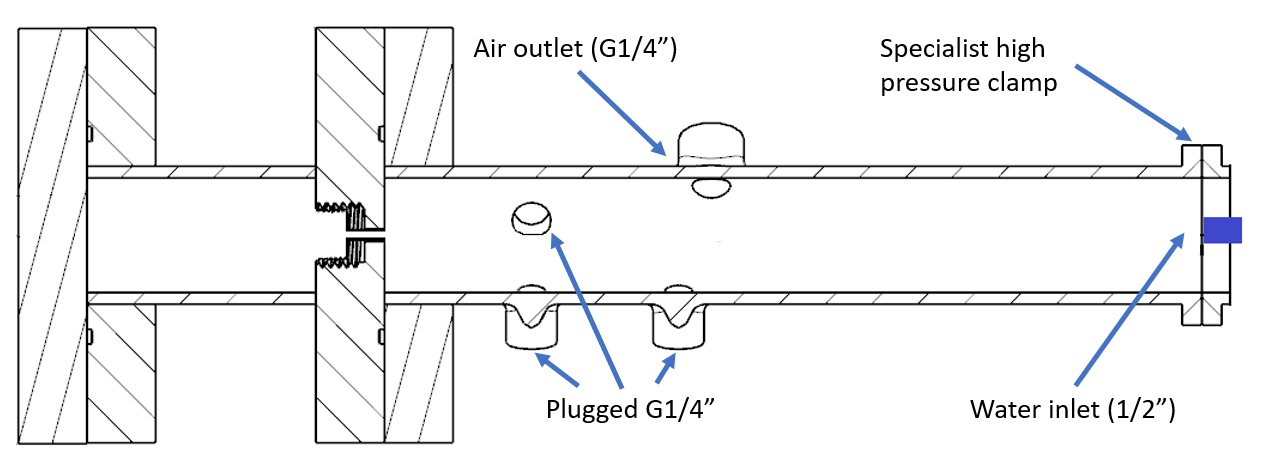
\includegraphics[width=1\textwidth]{hydro_test.png} 
	\caption{Shock tube drive section hydrostatic test schematic.}
	\label{fig:hydro_test}
\end{figure}

\begin{table}[H]
\centering
\caption{Hydrostatic test pressure values.}
\label{tab:hydro}
\begin{tabular}{@{}ll@{}}
\toprule
Device              & Pressure (Bar) \\ \midrule
Clamp rating        & 82             \\
Driver design       & 100            \\
Operational maximum & 25             \\
Test maximum        & $>80$          \\ \bottomrule
\end{tabular}
\end{table}



\subsubsection{Pressure Sensor Calibration}

Shock tube pressure measurements are typically taken using high speed, cylindrical pressure transducers placed flush to the section wall \citep{knight1958piezoelectric}. Mounting pressure transducers flush to the wall of the shock tube has classically been performed on square geometrical tubes \citep{knight1958piezoelectric, anderson2000shock,ryu1995shock}. Cylindrical shock tubes present a more complicated problem given the curved geometry of the section wall and flat sensing surface of the pressure transducer. For large cylindrical shock tubes this problem is negligible, but for small cylindrical shock tubes protrusions and recesses resulting from the presence of pressure traducers may have a major effect on the flow structure propagating through the tube.


\begin{figure}[H] 
	\centering
	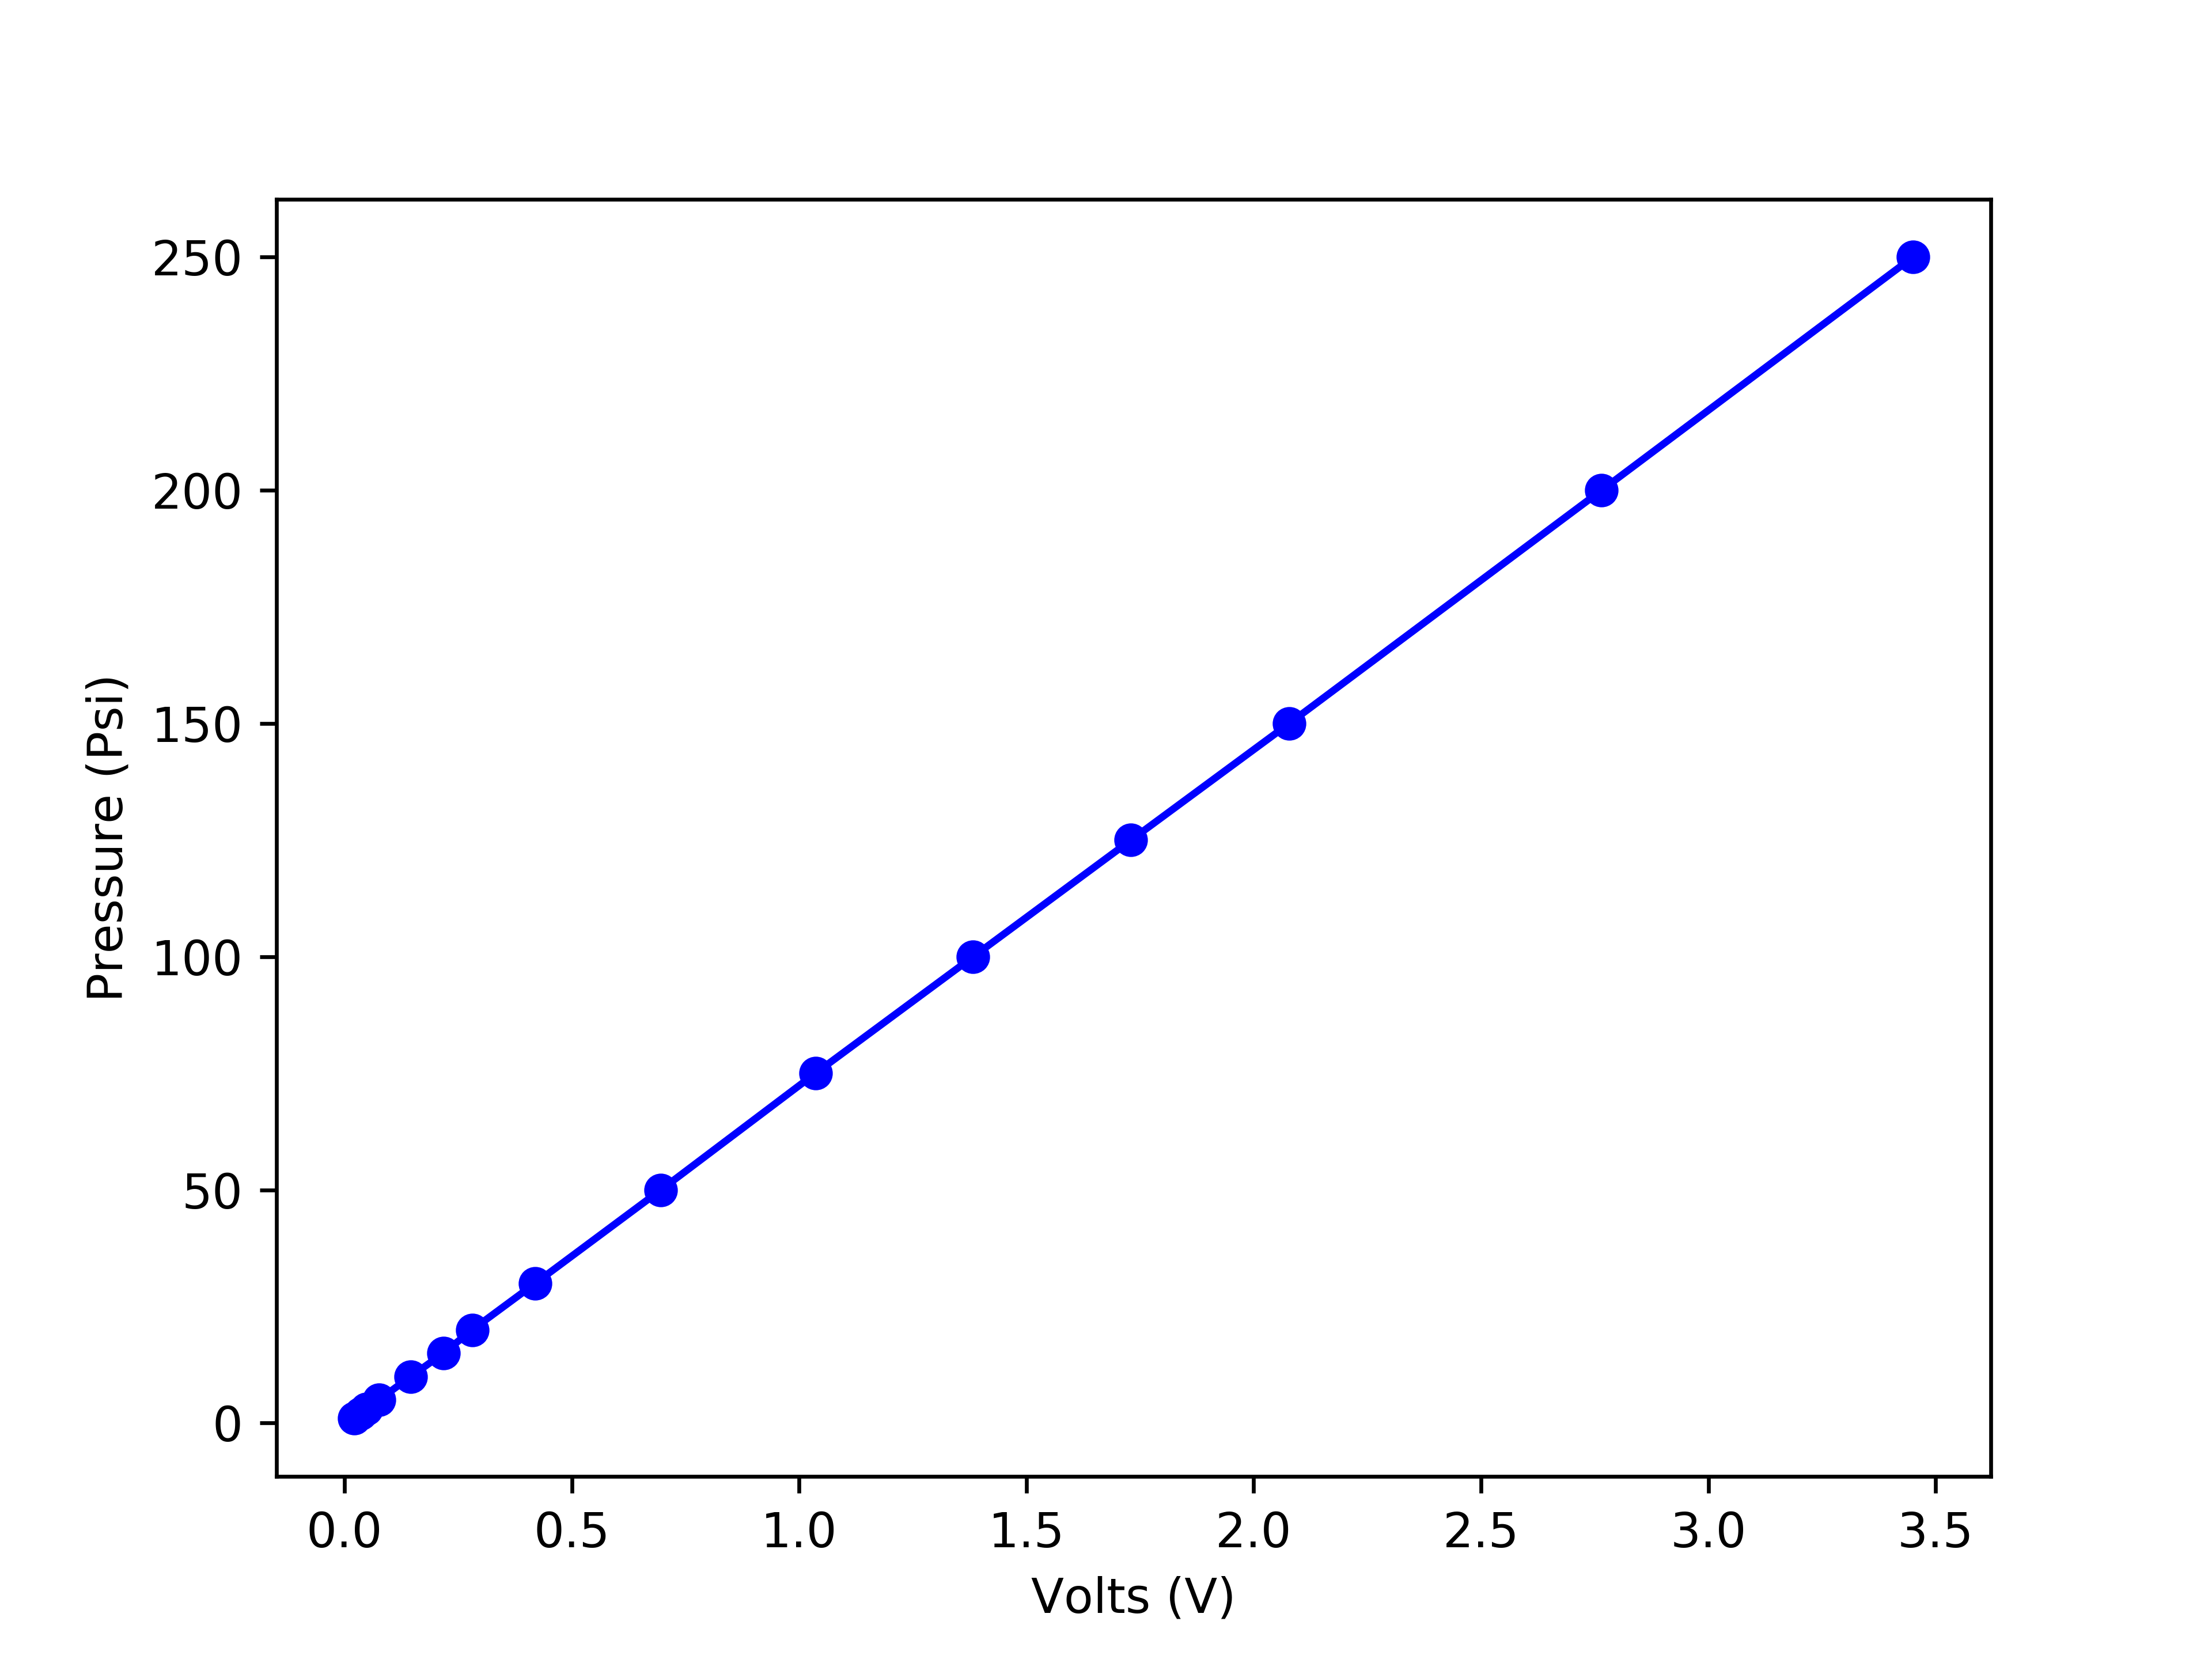
\includegraphics[width=0.88\textwidth]{pressure1.png} 
	\caption{Pressure sensor calibration data (in Psi).}
	\label{fig:hydro_test}
\end{figure}

\begin{figure}[H] 
	\centering
	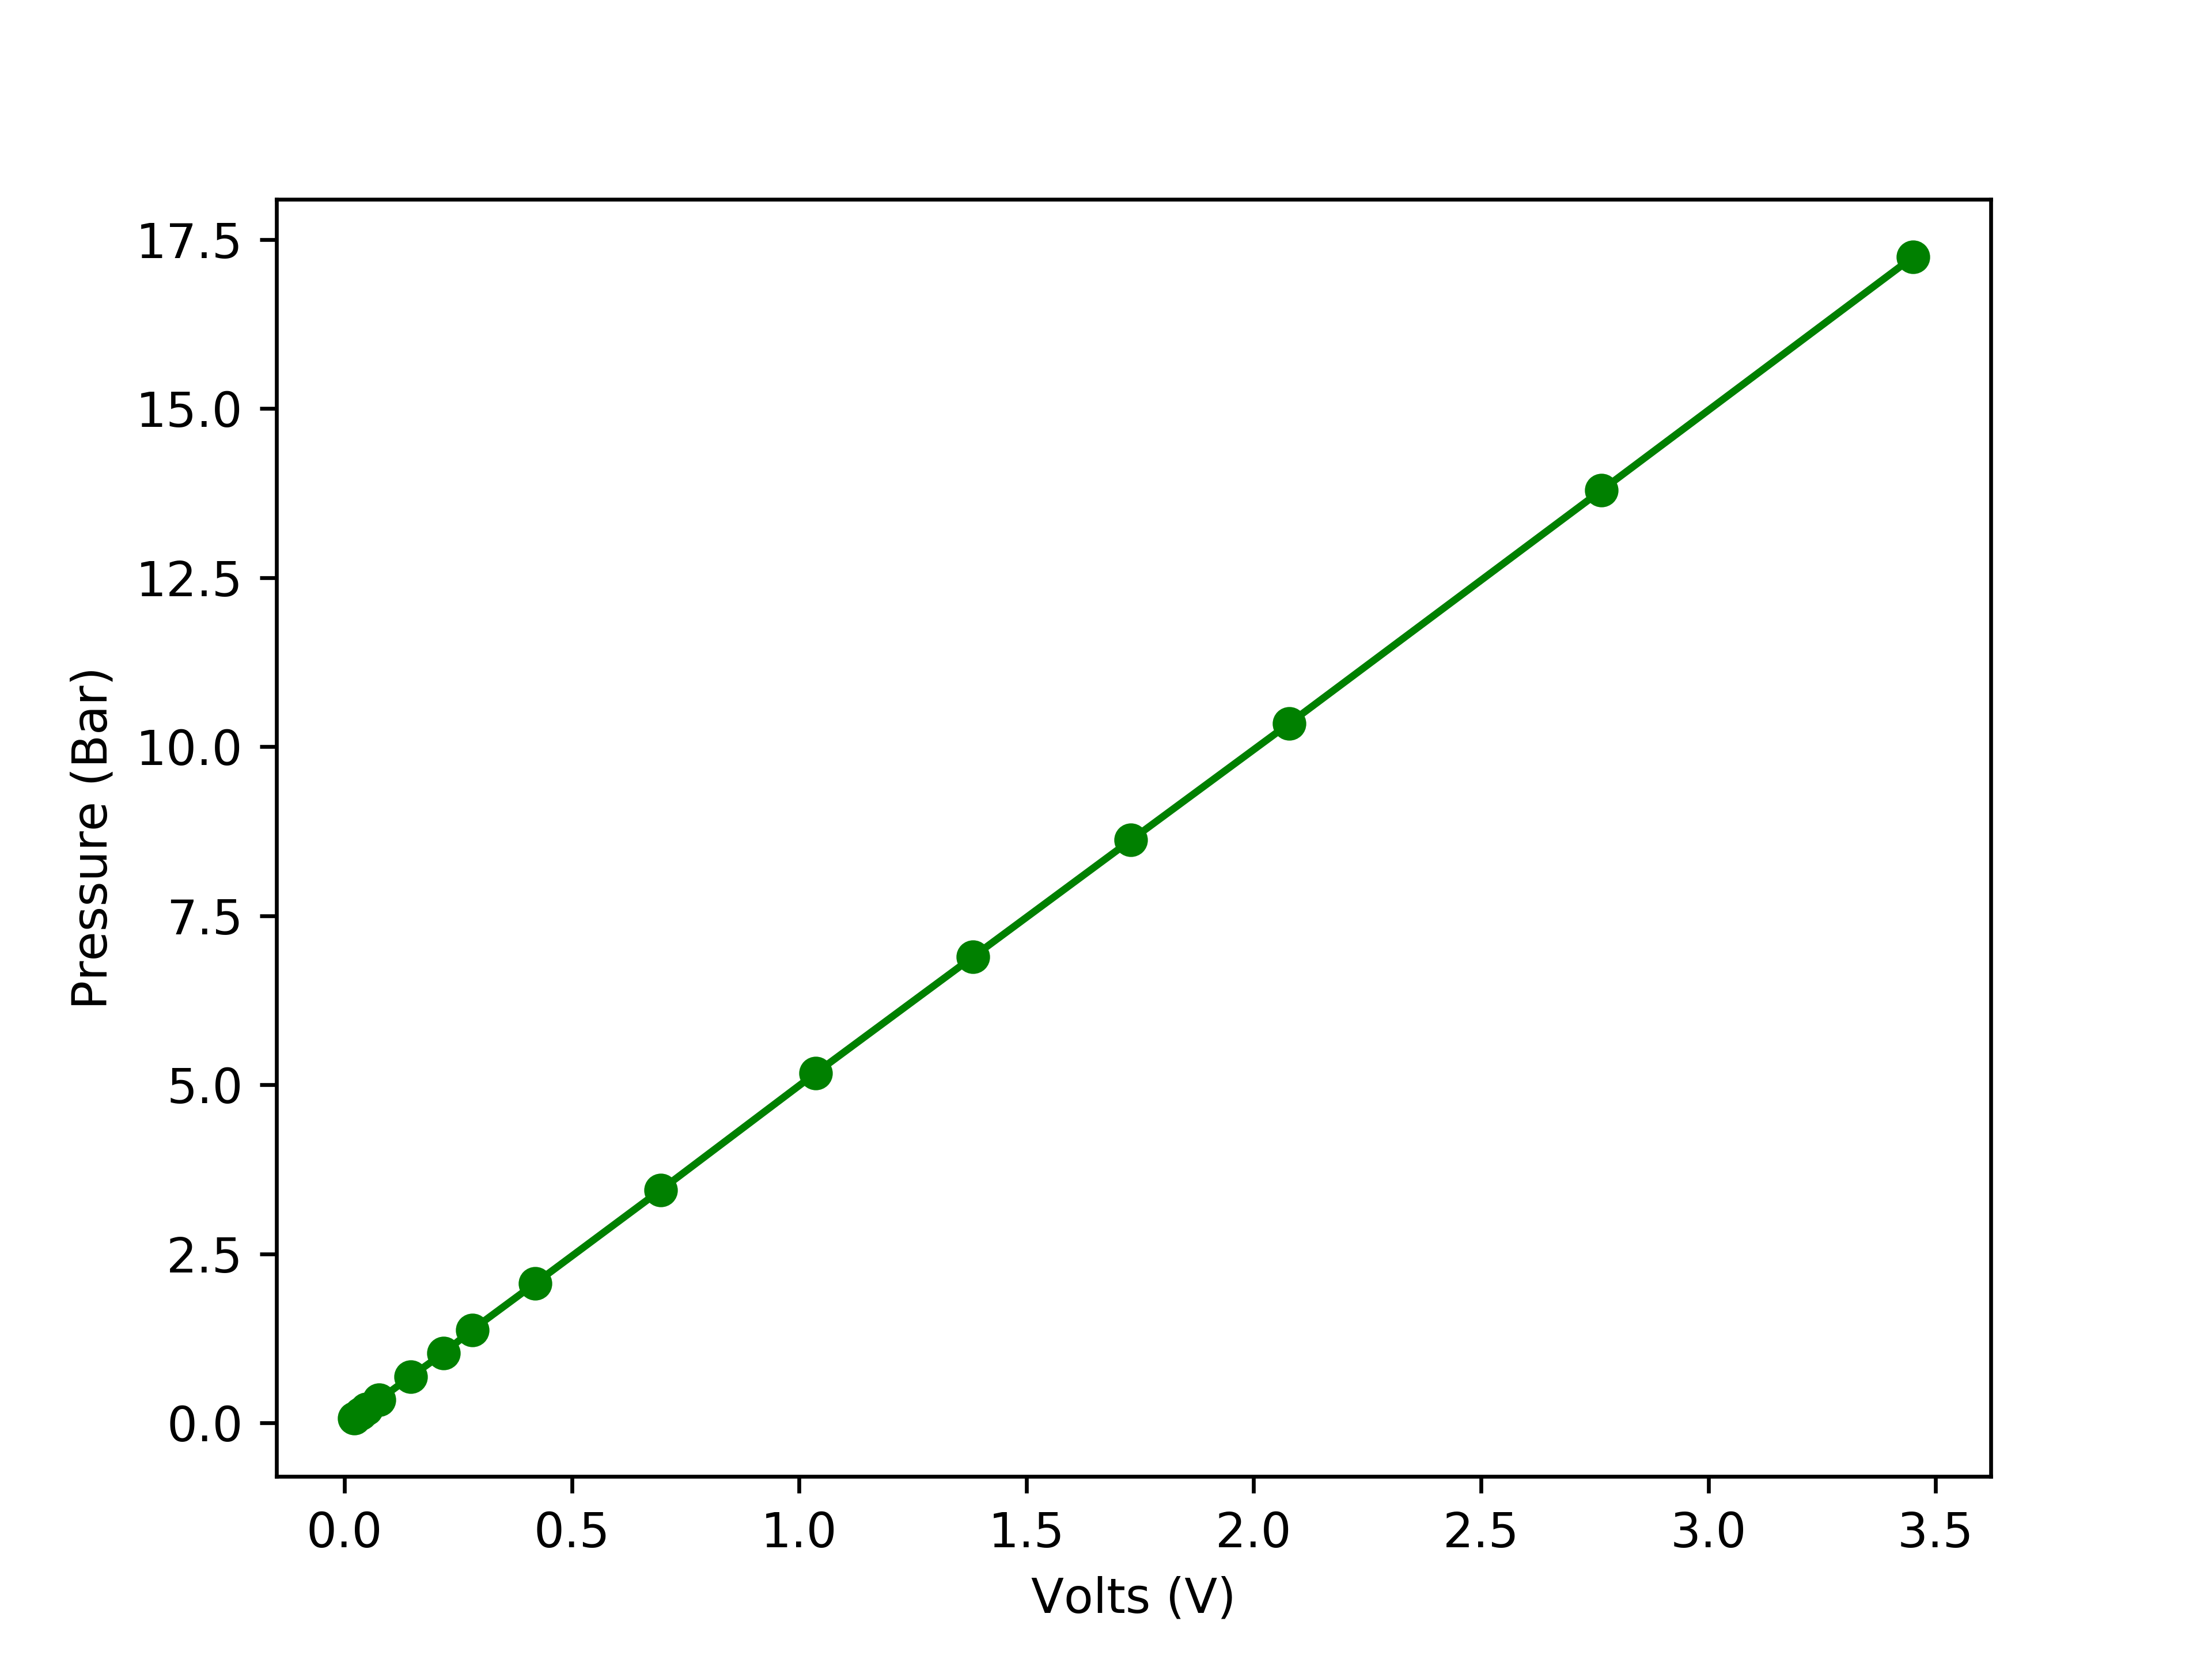
\includegraphics[width=0.88\textwidth]{pressure2.png} 
	\caption{Pressure sensor calibration data (in Bar).}
	\label{fig:hydro_test}
\end{figure}

\subsubsection{Diaphragm Study}

\subsubsection{LED Calibration}
The pulsed light emitting diode (LEDs) provides the necessary light source required to capture density gradients present within the evolution of the transient supersonic jet and following flow structures. The pulsed LED source is operated by a simple driver circuit and is modulated to supply a constant pulse width within the input voltage limitations of the specific LED. The LED produces a narrow emission bandwidth which reduces chromatic aberrations that is still spectrally wide enough to prevent the appearance of diffraction effects in captured images \citep{willert2012assessment}. Light provided by a LED is emitted within nanoseconds and is essentially lag-free unlike historically used light sources such as lasers or discharge lamps. The amount of light supplied to a schlieren system dictates the quality of a captured image. Equation \ref{eqn:blur} highlights the relation between the speed of the exiting flow $U_i$, the length of the image window $X_{image}$, the pulse width of the LED $T_{LED}$, and the percentage of blur captured in the image. Figure \ref{fig:pulse} shows that as the pulse width increases so does the image blur. This is a result of an over-saturation of light and subsequent blurring of the image. If the pulse width is decreased the image suffers a shortage of light and appears grainy. A pulse width value is determined sufficient based on the desired outcome of a captured image. For a clear representation of flow structures a slightly higher pulse width may be used whereas, for the accurate analysis of stock structure propagation blurring is undesirable and a lower pulse width value will be implemented. Using equation \ref{eqn:blur}, (a) and (b) from Figure \ref{fig:pulse} displays a percentage blur of 10\% and 2\% respectively. It was found that analytically this was not suitable. Figure \ref{fig:pulse_f} shows an underexpanded jet for a pulse width of 0.8ms, this value was found acceptable for data extraction analytic tools and detailed flow structure discussions.



\begin{equation} \label{eqn:blur}
\%_{blur} = \frac{U_i}{T_{LED}*X_{image}}
\end{equation}
\begin{figure}[H]
  \centering
  \subfloat[Pulse width = 5ms.]{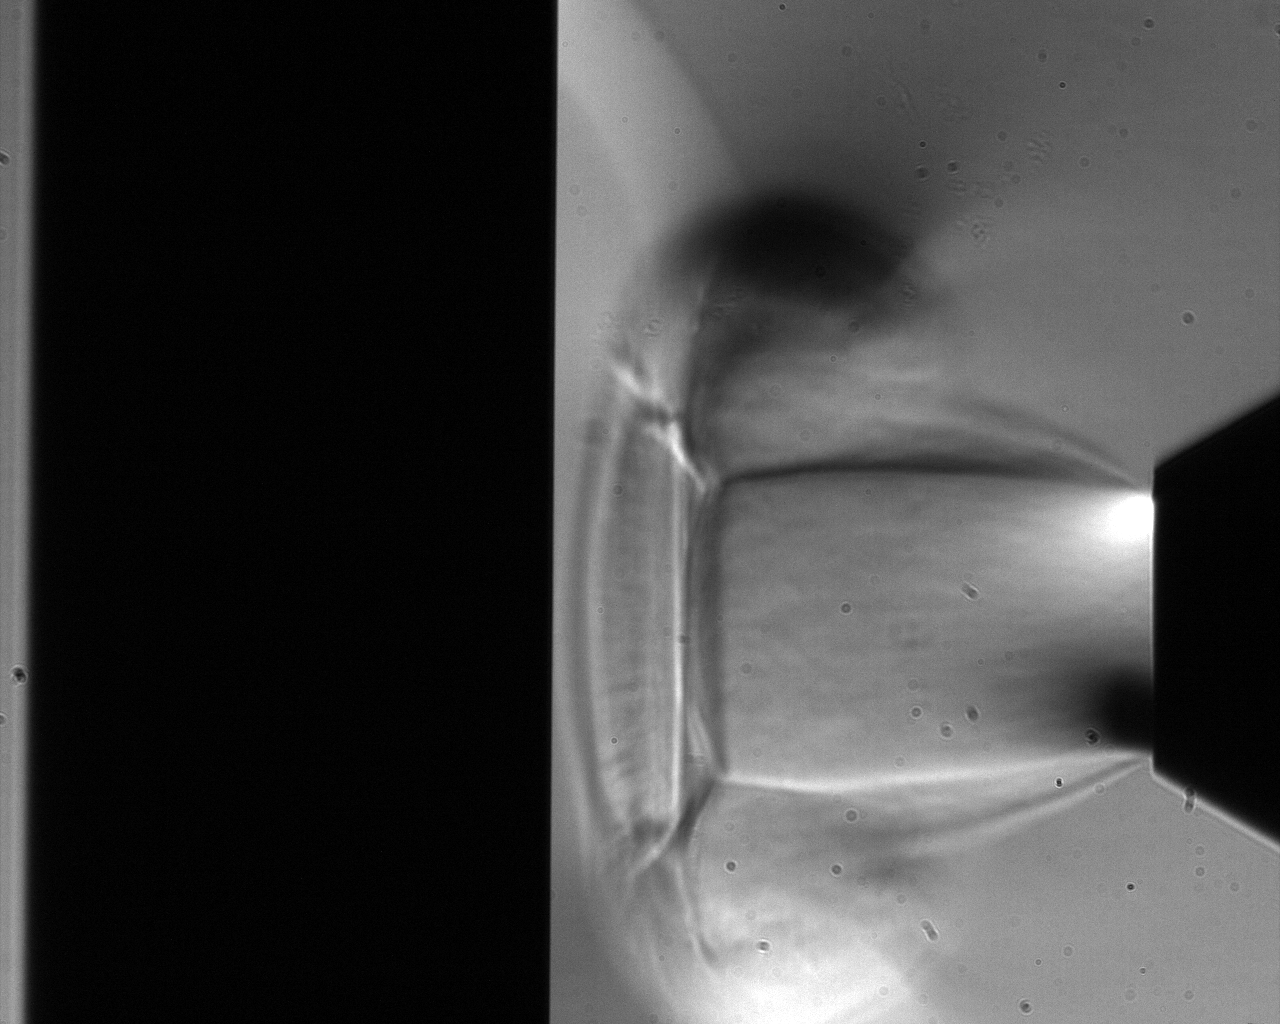
\includegraphics[width=0.48\textwidth]{blur_example.png}}
  \hfill
  \subfloat[Pulse width = 0.5ms.]{
\includegraphics[width=0.48\textwidth]{grain_example.png}}
  \caption{Pulse width study.}
  \label{fig:pulse}
\end{figure}

%\begin{figure}[H] 
%	\centering
%	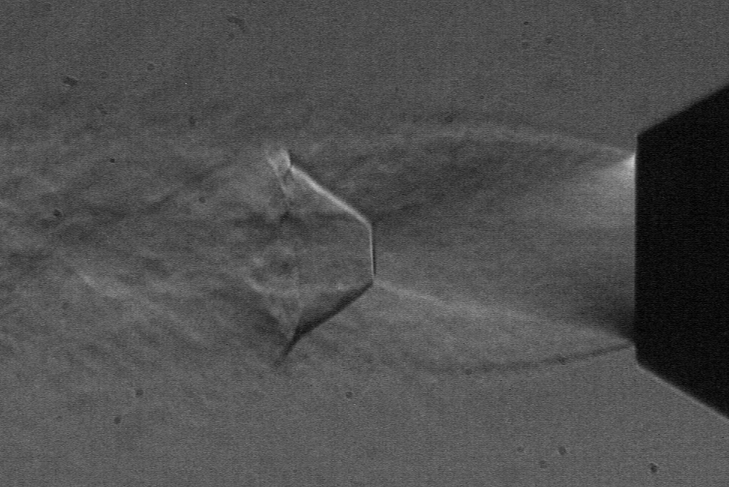
\includegraphics[width=0.88\textwidth]{pulse.png} 
%	\caption{Underexpanded shock for a pulse width of 0.8ms.}
%	\label{fig:pulse_f}
%\end{figure}


\newpage

\section{Analysis Techniques} \label{sect:post}

Schlieren imaging produces a path integrated density gradient image that is excellent for flow visualisation however, it is difficult to quantitatively extract physical parameters directly from image data. Extracting features and data from images requires a pipe line of different image processing techniques. This section outlines each processing technique and its application to the image data.

\subsection{Second Order Convolution}
The first step of the flow feature extraction pipeline is to find a set of distinctive
structures that can be reliably localized under varying imaging conditions including image translation and rotation, and background noise. It is not a simple task to meet these criteria for instance, if a point is located in a uniform region an algorithm will not be able to use neighbouring points to distinguish the structure of interest. Similarly, analysing a straight line structure will only yield motion information perpendicular to the line. These limitations motivate the investigation of points in non-uniform environments exhibiting signal variations in two directions. The Hessian detector \citep{beaudet1978rotationally} searches for image structures that exhibit strong derivatives in two orthogonal directions. Second order image derivatives are computed by convolution using second order derivatives of the Gaussian kernel \citep{lindeberg1994linear}. The second order derivative of the Gaussian operator reduces  noise present in the raw image, and smooths the background to a degree dependent on the smoothing parameter $\sigma$. Mathematically this means that if f denotes the image and G the normalised Gaussian the algorithm computes

\begin{equation}
f_{ij}(x,\sigma) = (f*G_{ij})(x,\sigma)
\end{equation}

with,

\begin{equation}
G_{ij}(x,\sigma)=\left(\frac{\delta^2}{\delta_i\delta_j}G\right)(x,\sigma)
\end{equation}

where * denotes spatial convolution, x=(x,y) denotes the pixel position, and the derivative directions i and j can be any combination of x and y. The eigenvectors and eigenvalues are computed in the algorithm from a second derivative Hessian matrix.

\begin{equation} \label{eqn:hessian}
H_f=
  \begin{bmatrix}
    f_{xx}(x,\sigma) & f_{xy}(x,\sigma) \\
    f_{xy}(x,\sigma) & f_{yy}(x,\sigma)
  \end{bmatrix}
\end{equation}

The Hessian detector computes the second derivatives $f_{xx}$, $f_{xy}$, and $f_{yy}$ for each image point and then searches for points where the determinant of the Hessian becomes maximal.
\begin{equation}
det(H_f)= f_{xx}f_{yy}-f_{xy}^2
\end{equation}

Figure \ref{fig:hessian_app} highlights the correspondence between eigenvalues of the Hessian detector and local features of the image such as corners, edges, or flat regions. Table \ref{tab:hessian} highlights the relation between the magnitude of Hessian matrix eigenvalues and the corresponding image structures that will be detected in 3-dimensional images.

\begin{figure}[H] 
	\centering
	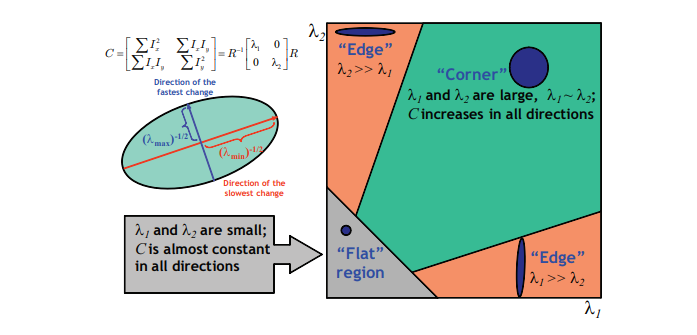
\includegraphics[width=1\textwidth]{hessian_app.png} 
	\caption{Correspondence between eigenvalues of the Hessian operation and local features (corners, edges, flat regions) \citep{grauman2011visual}.}
	\label{fig:hessian_app}
\end{figure}


\begin{table}[H]
\centering
\caption{"Eigenvalues of the Hessian matrix and image structure
orientation (L low, H+ high positive, H- high negative)" \citep{rudzki2009vessel}.}
\label{tab:hessian}
\begin{tabular}{@{}llll@{}}
\toprule
$\lambda_1$ & $\lambda_2$ & $\lambda_3$ & Structure orientation          \\ \midrule
L           & L           & L           & noise (no preferred structure) \\
L           & L           & H-          & bright sheet-like structure    \\
L           & L           & H+          & dark sheet-like structure      \\
L           & H-          & H-          & bright tubular structure       \\
L           & H+          & H+          & dark tubular structure         \\
H-          & H-          & H-          & bright blob-like structure     \\
H+          & H+          & H+          & dark blob-like structure       \\ \bottomrule
\end{tabular}
\end{table}

Figure \ref{fig:hessian_img} shows the application of a second order convolution on raw transient supersonic jet image data. A smoothing parameter of $\sigma=2$ was chosen as an acceptable value after a variable sweep was conducted, Figure \ref{fig:hessian_var} shows the degree of smoothing for several $\sigma$ values. Appendix \ref{app:code} details the algorithm used for this process and Appendix \ref{app:hessian} presents the application of the algorithm on the entire transient supersonic jet process.

\begin{figure}[H]
  \centering
  \subfloat[$\sigma=1$.]{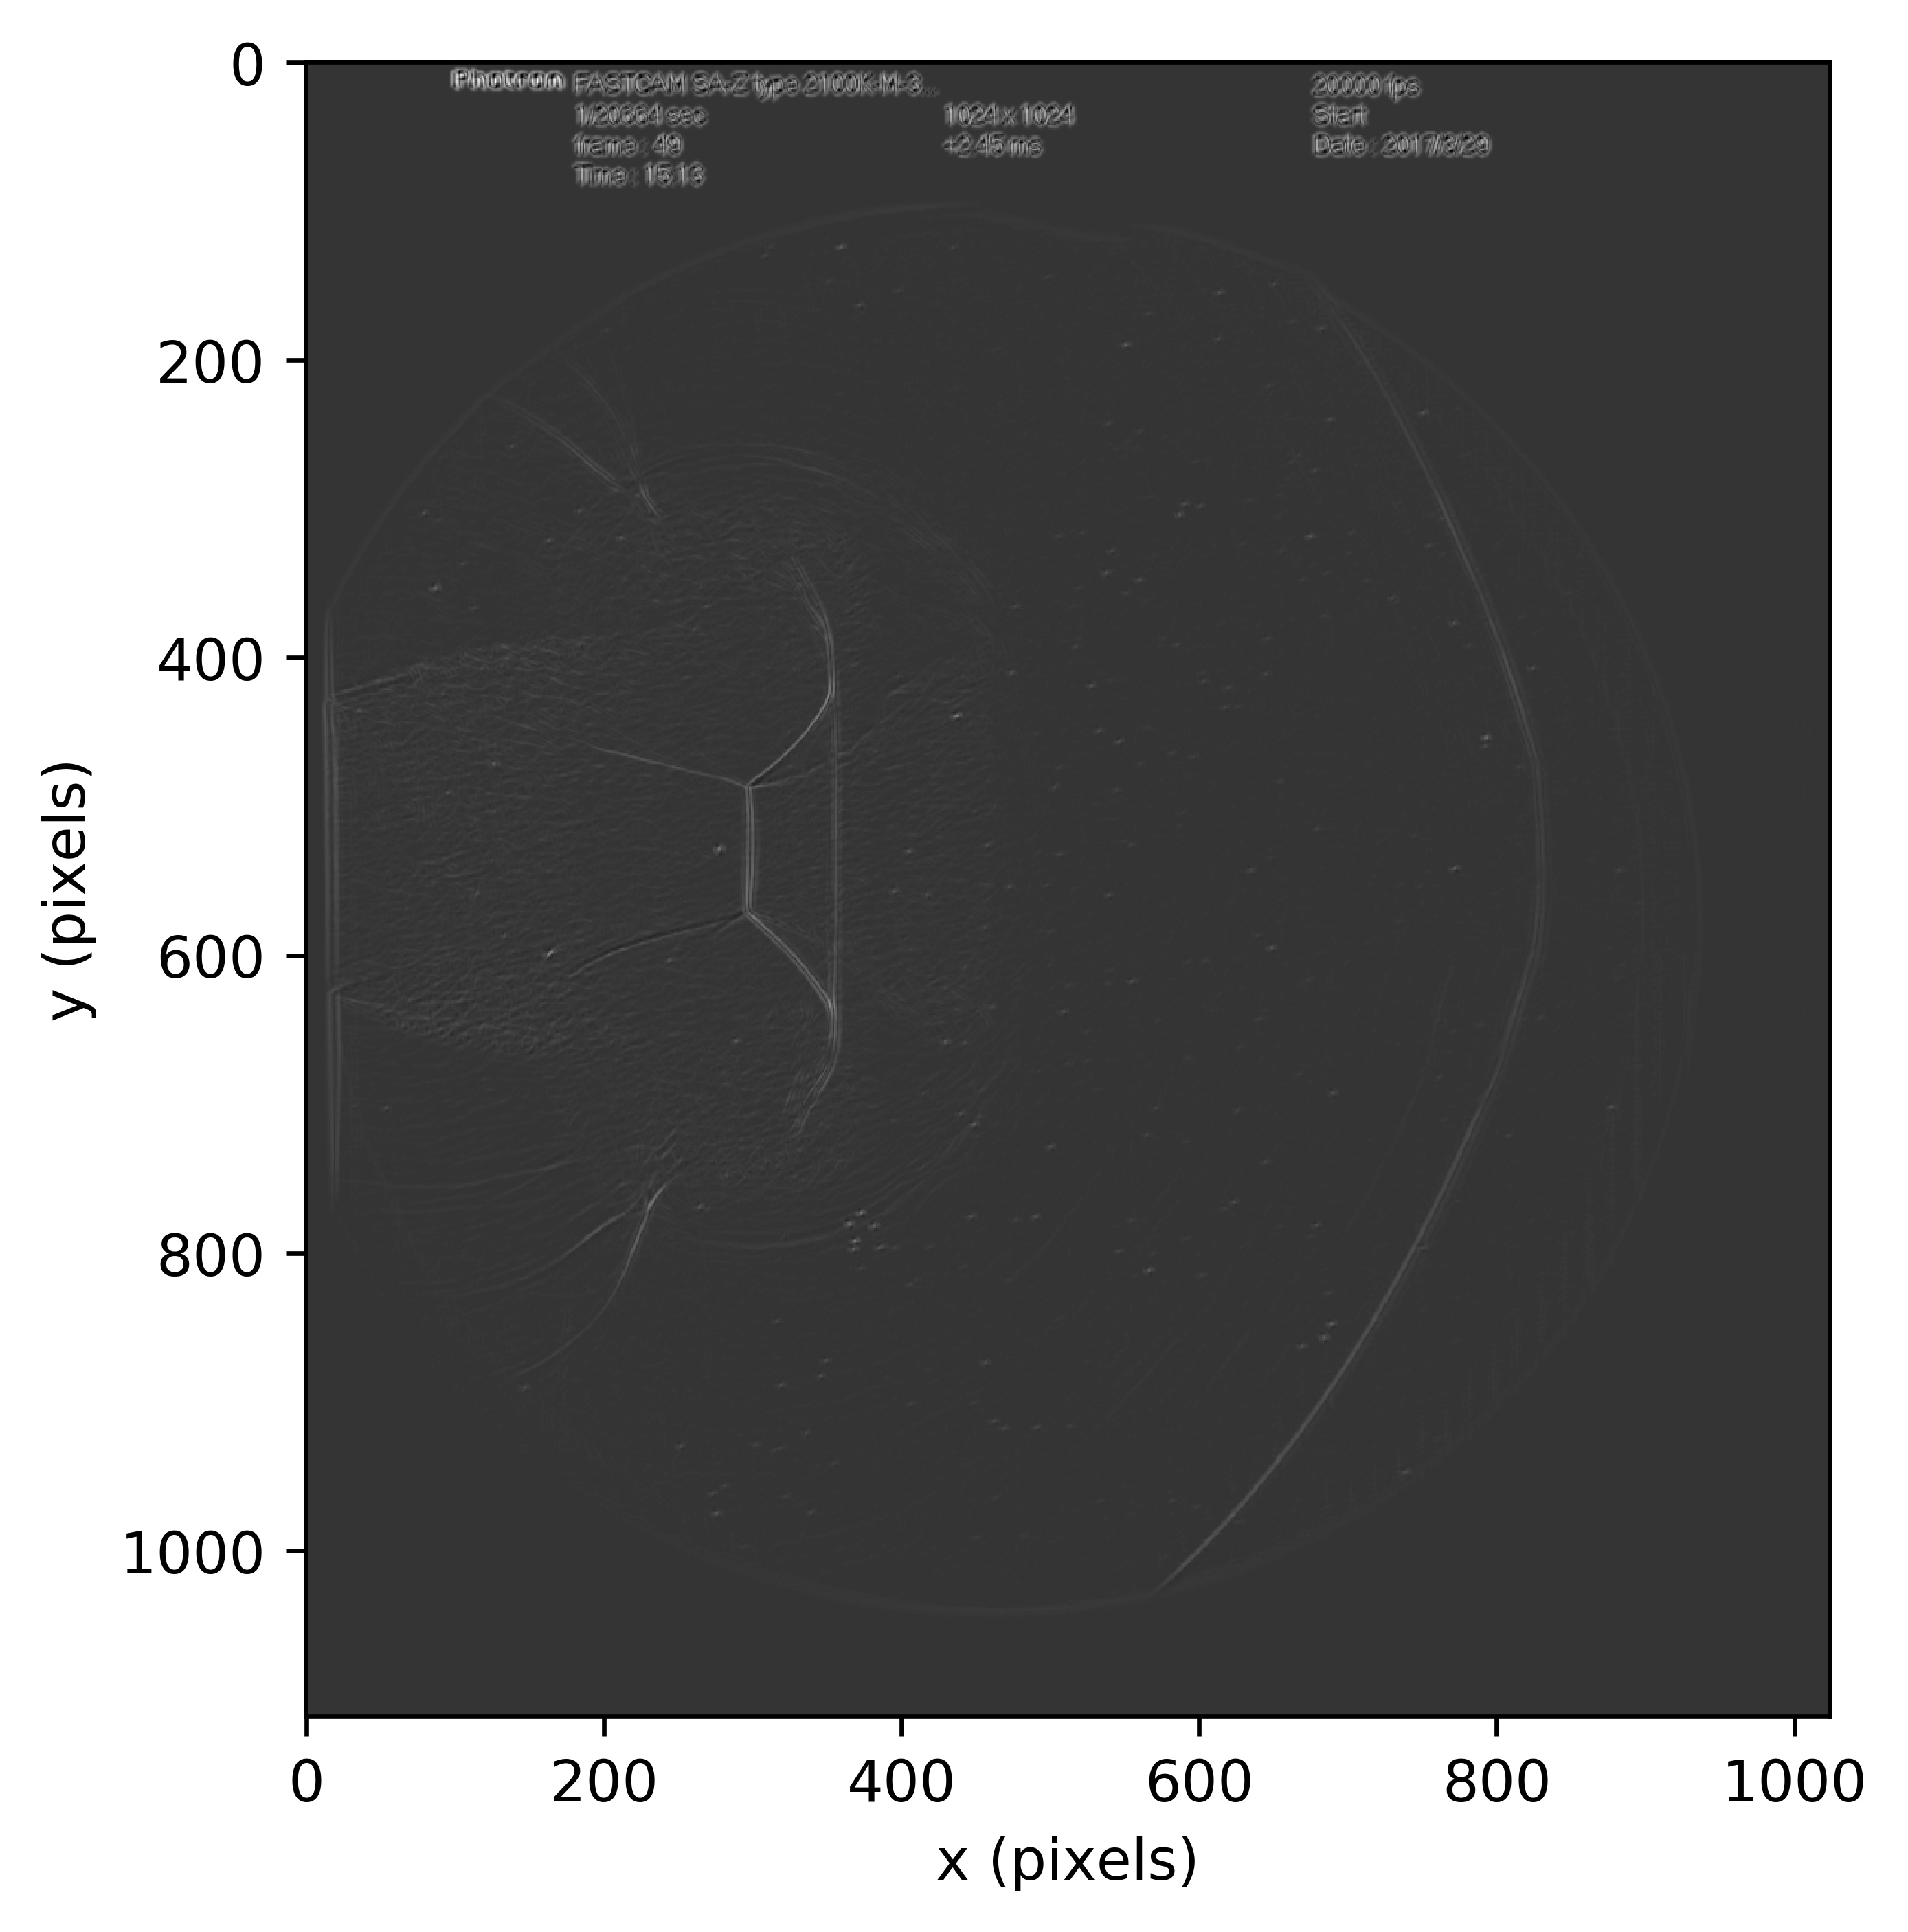
\includegraphics[width=0.5\textwidth]{sigma_1.jpg}}
  \hfill
  \subfloat[$\sigma=2$.]{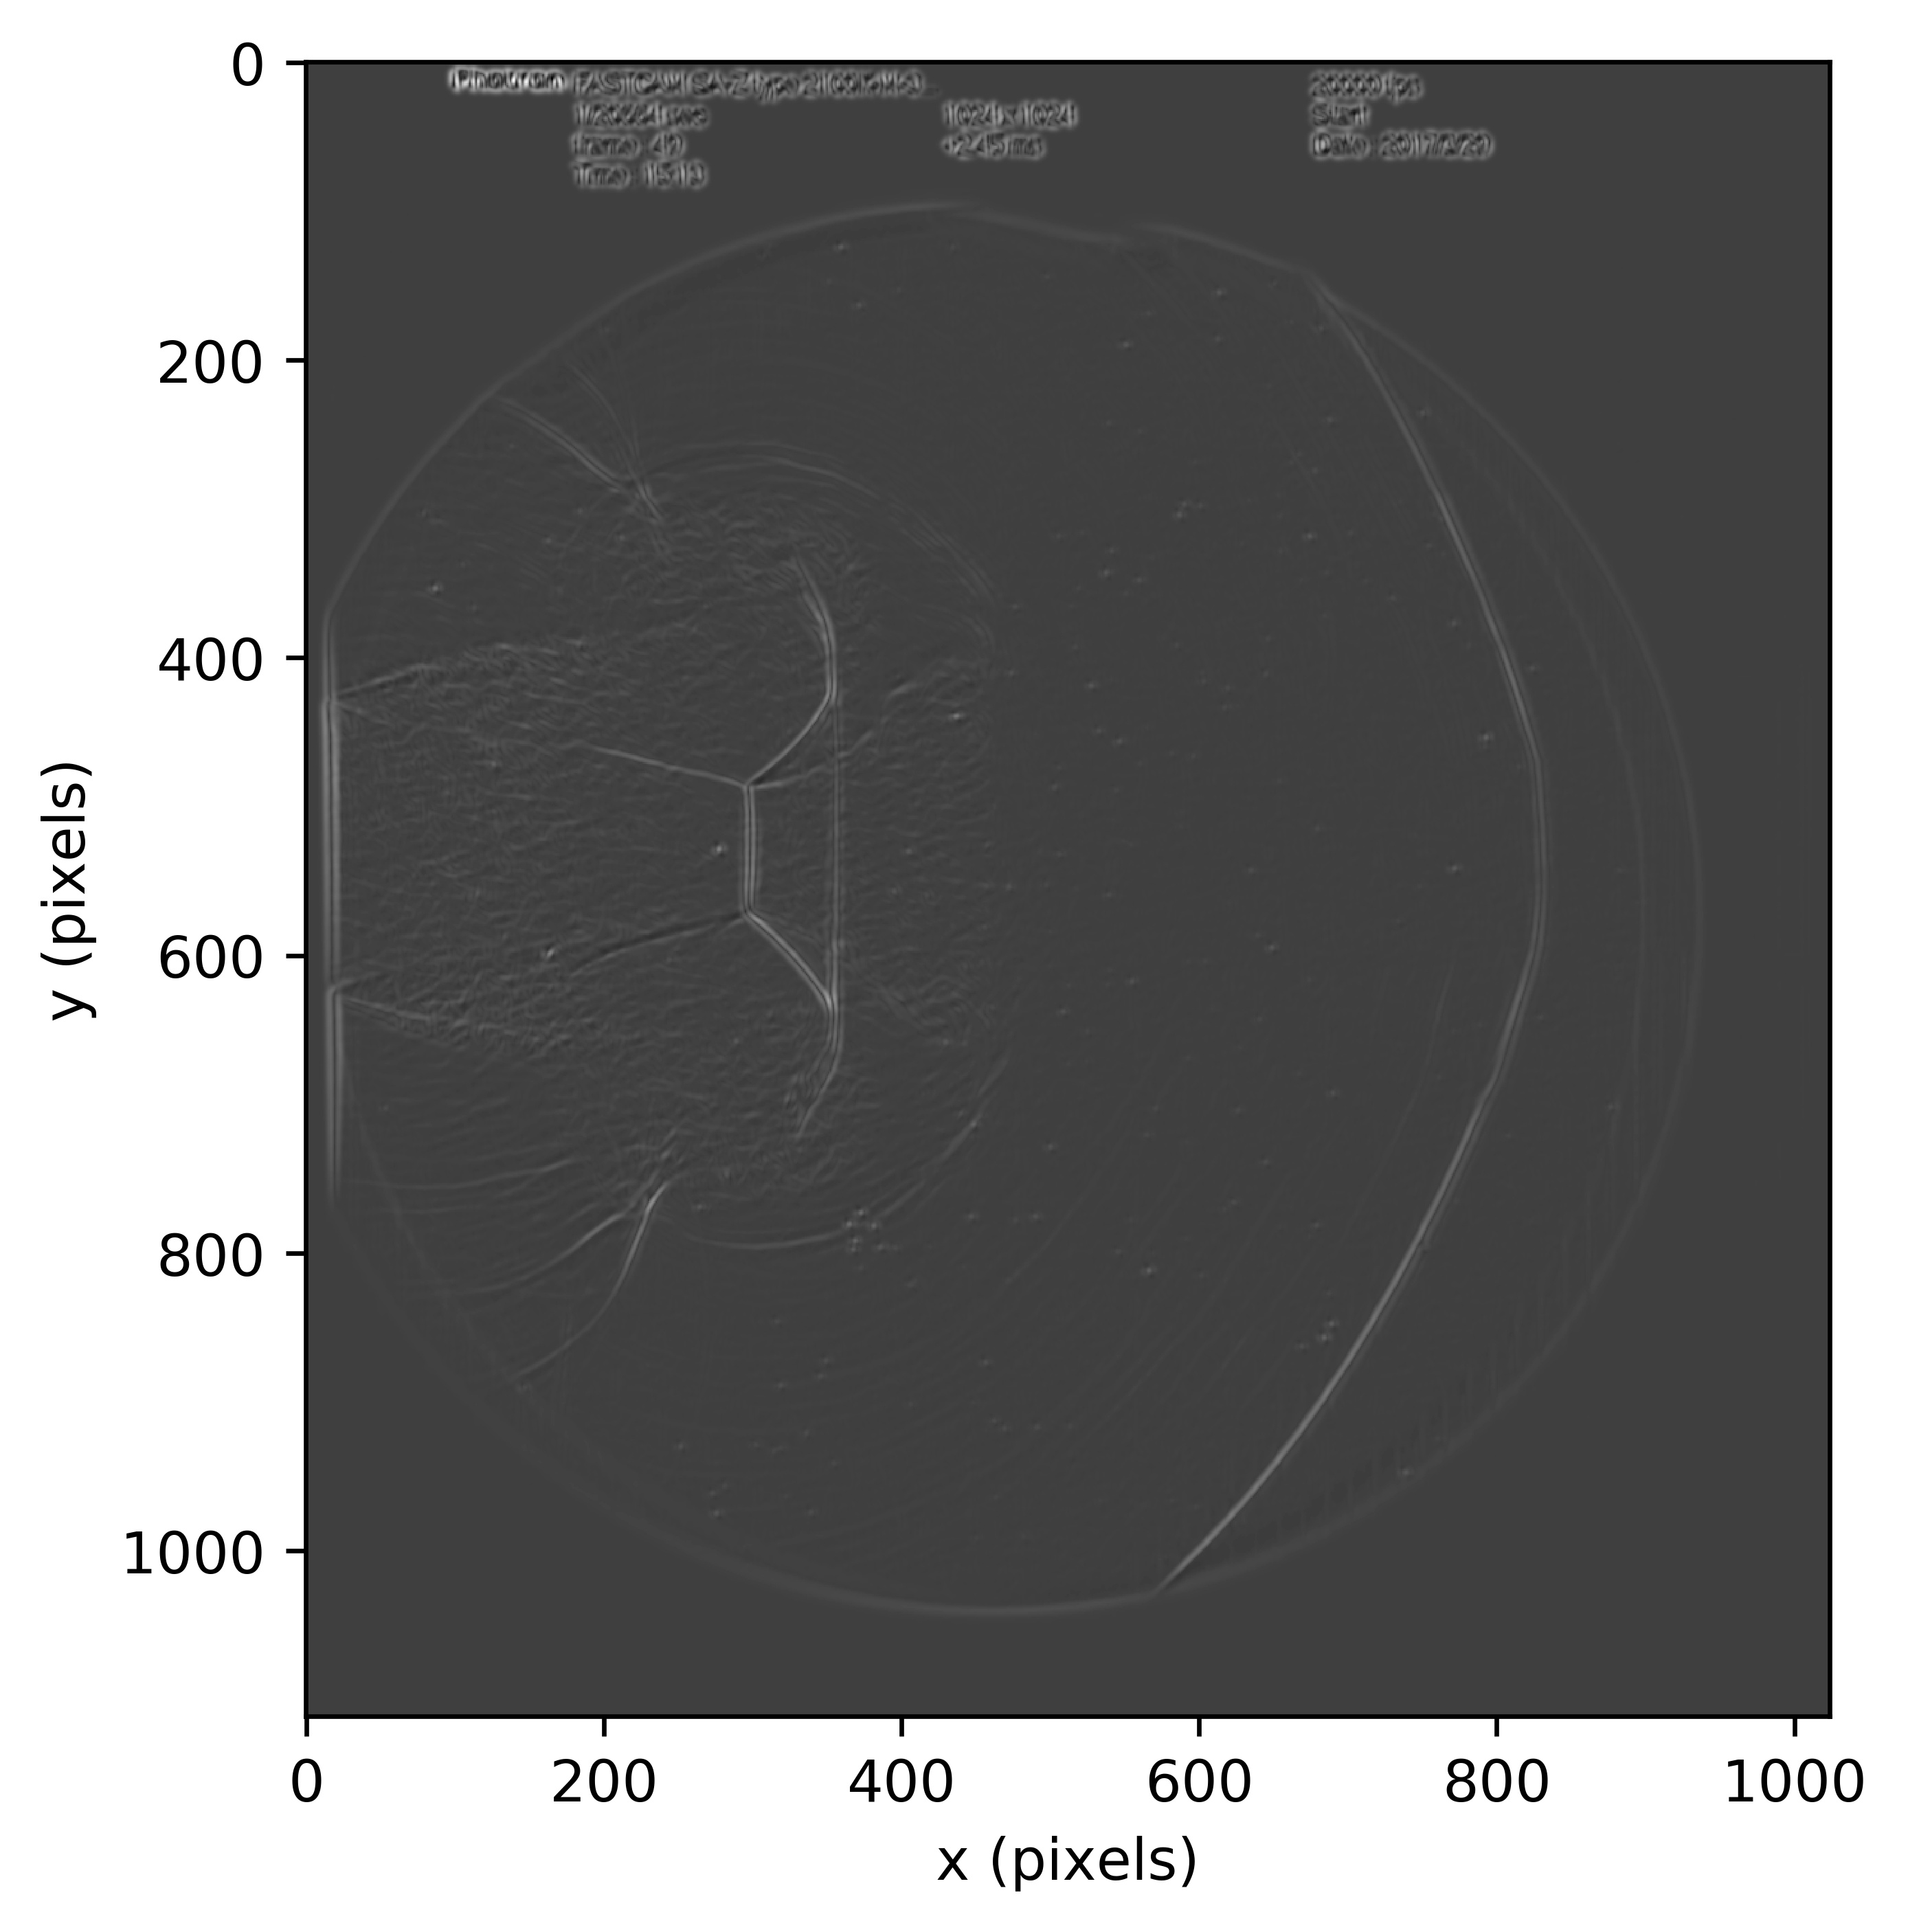
\includegraphics[width=0.5\textwidth]{sigma_2.jpg}}\\
  \subfloat[$\sigma=3$.]{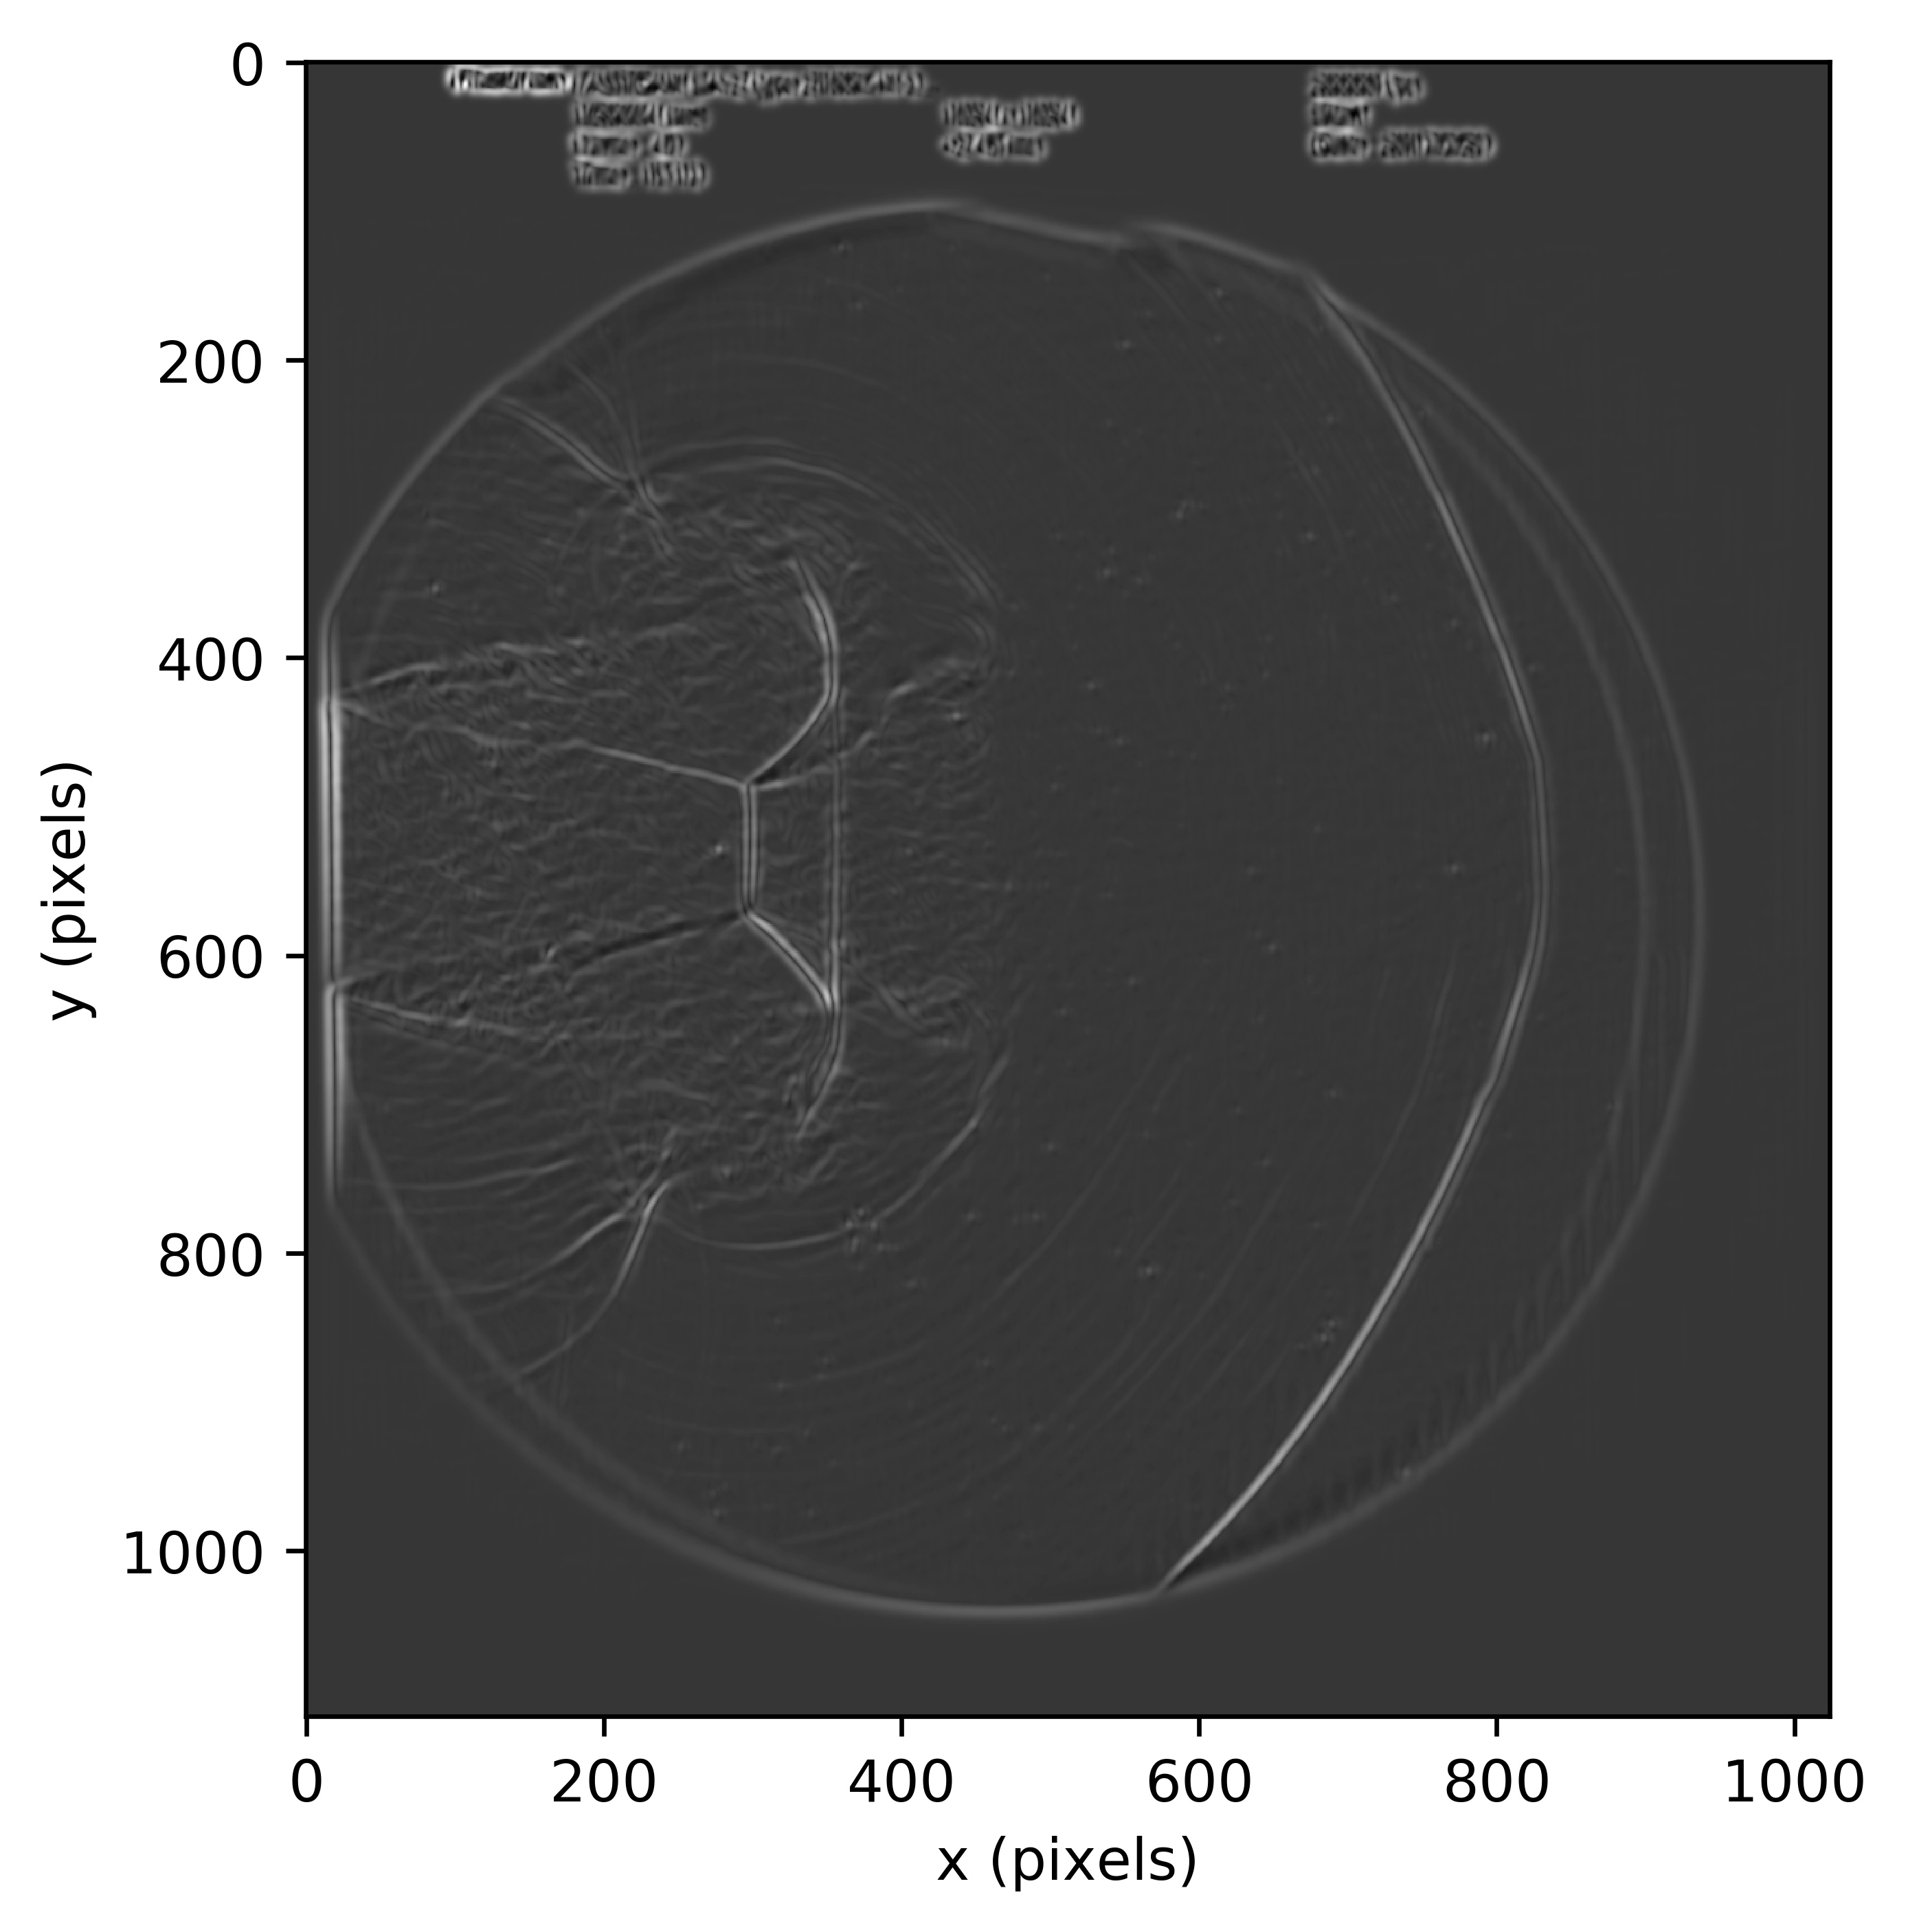
\includegraphics[width=0.5\textwidth]{sigma_3.jpg}}
  \hfill
  \subfloat[$\sigma=4$.]{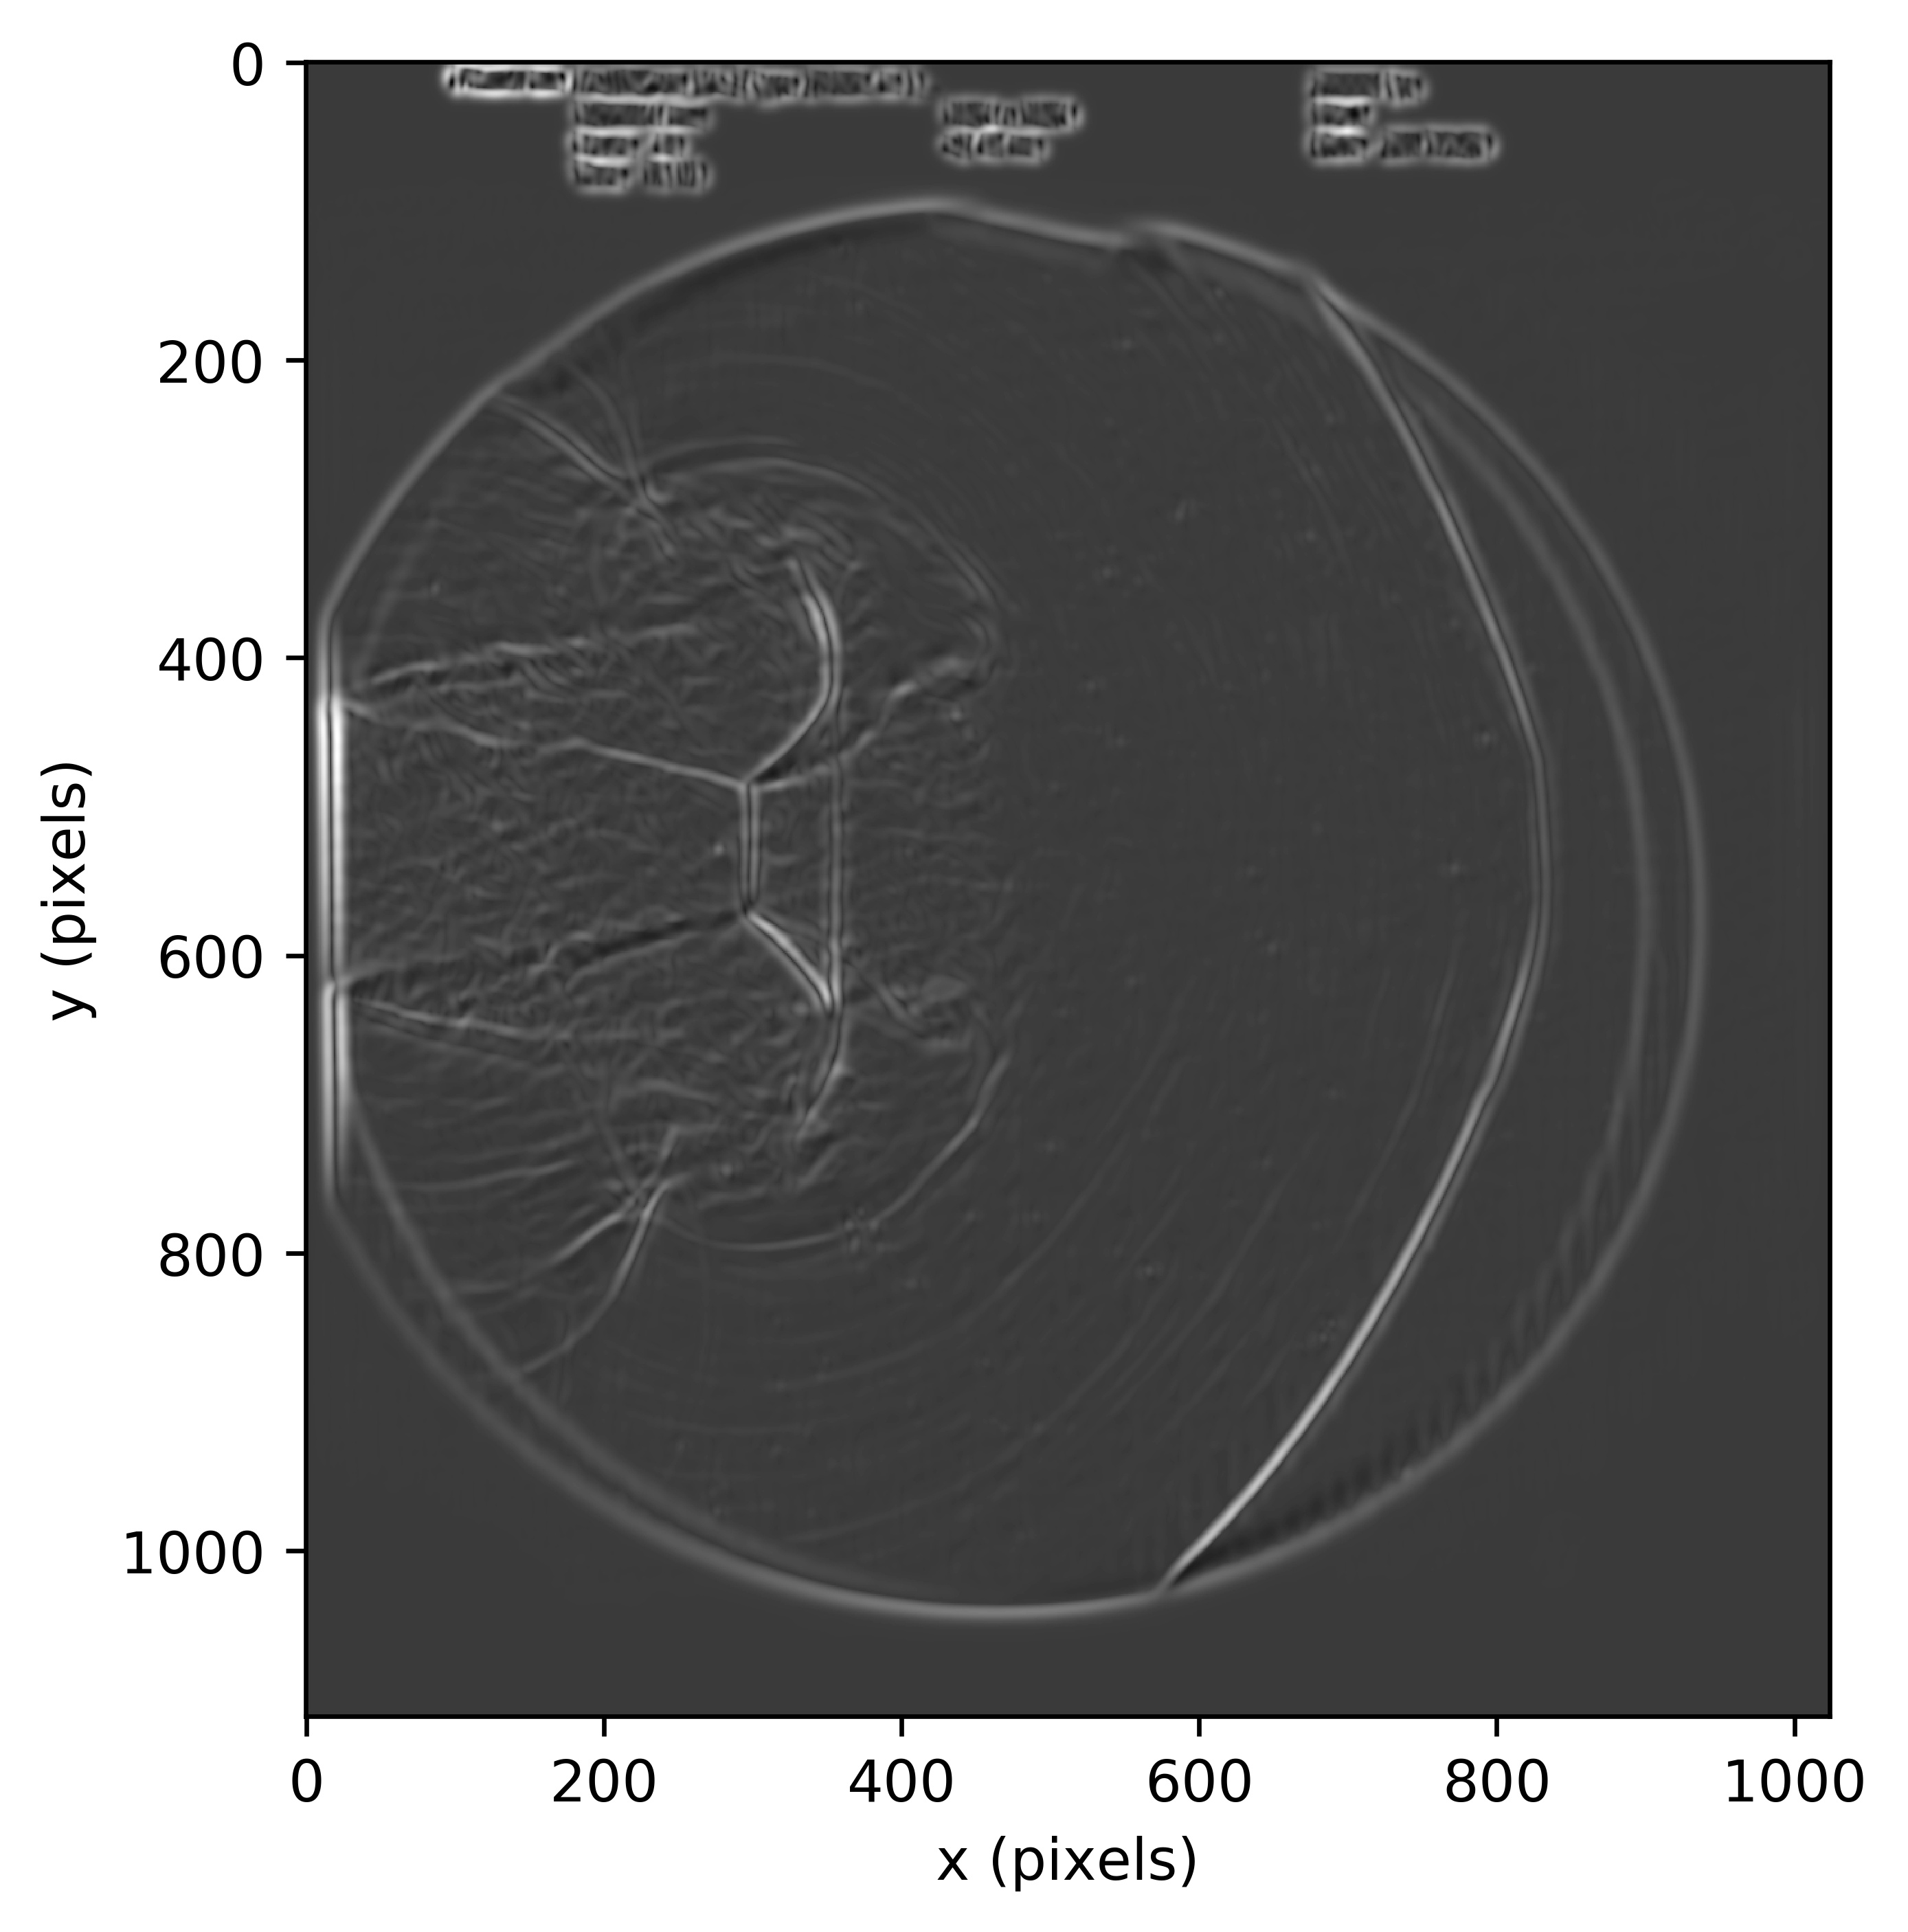
\includegraphics[width=0.5\textwidth]{sigma_4.jpg}}
  \caption{Smoothing parameter sweep.}
  \label{fig:hessian_var}
\end{figure}

\begin{figure}[H]
  \centering
  \subfloat[Input image .]{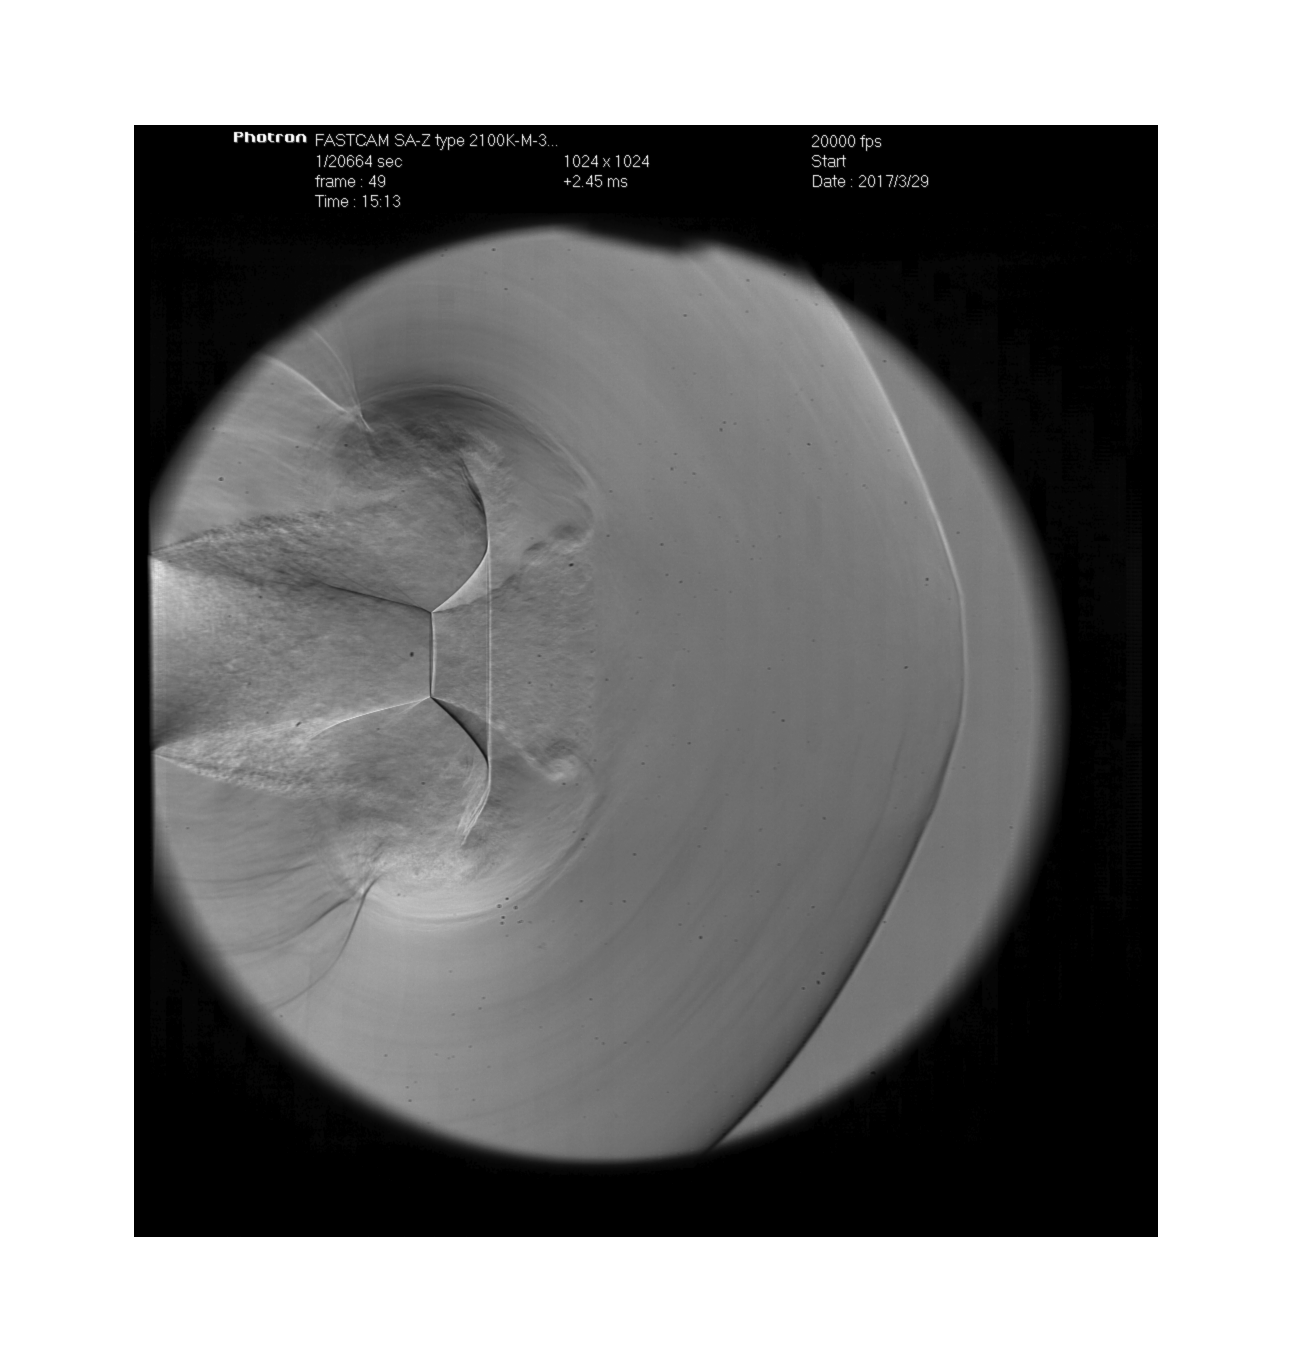
\includegraphics[width=0.5\textwidth]{vid89_frame50.png}}
  \hfill
  \subfloat[$\sigma=2$.]{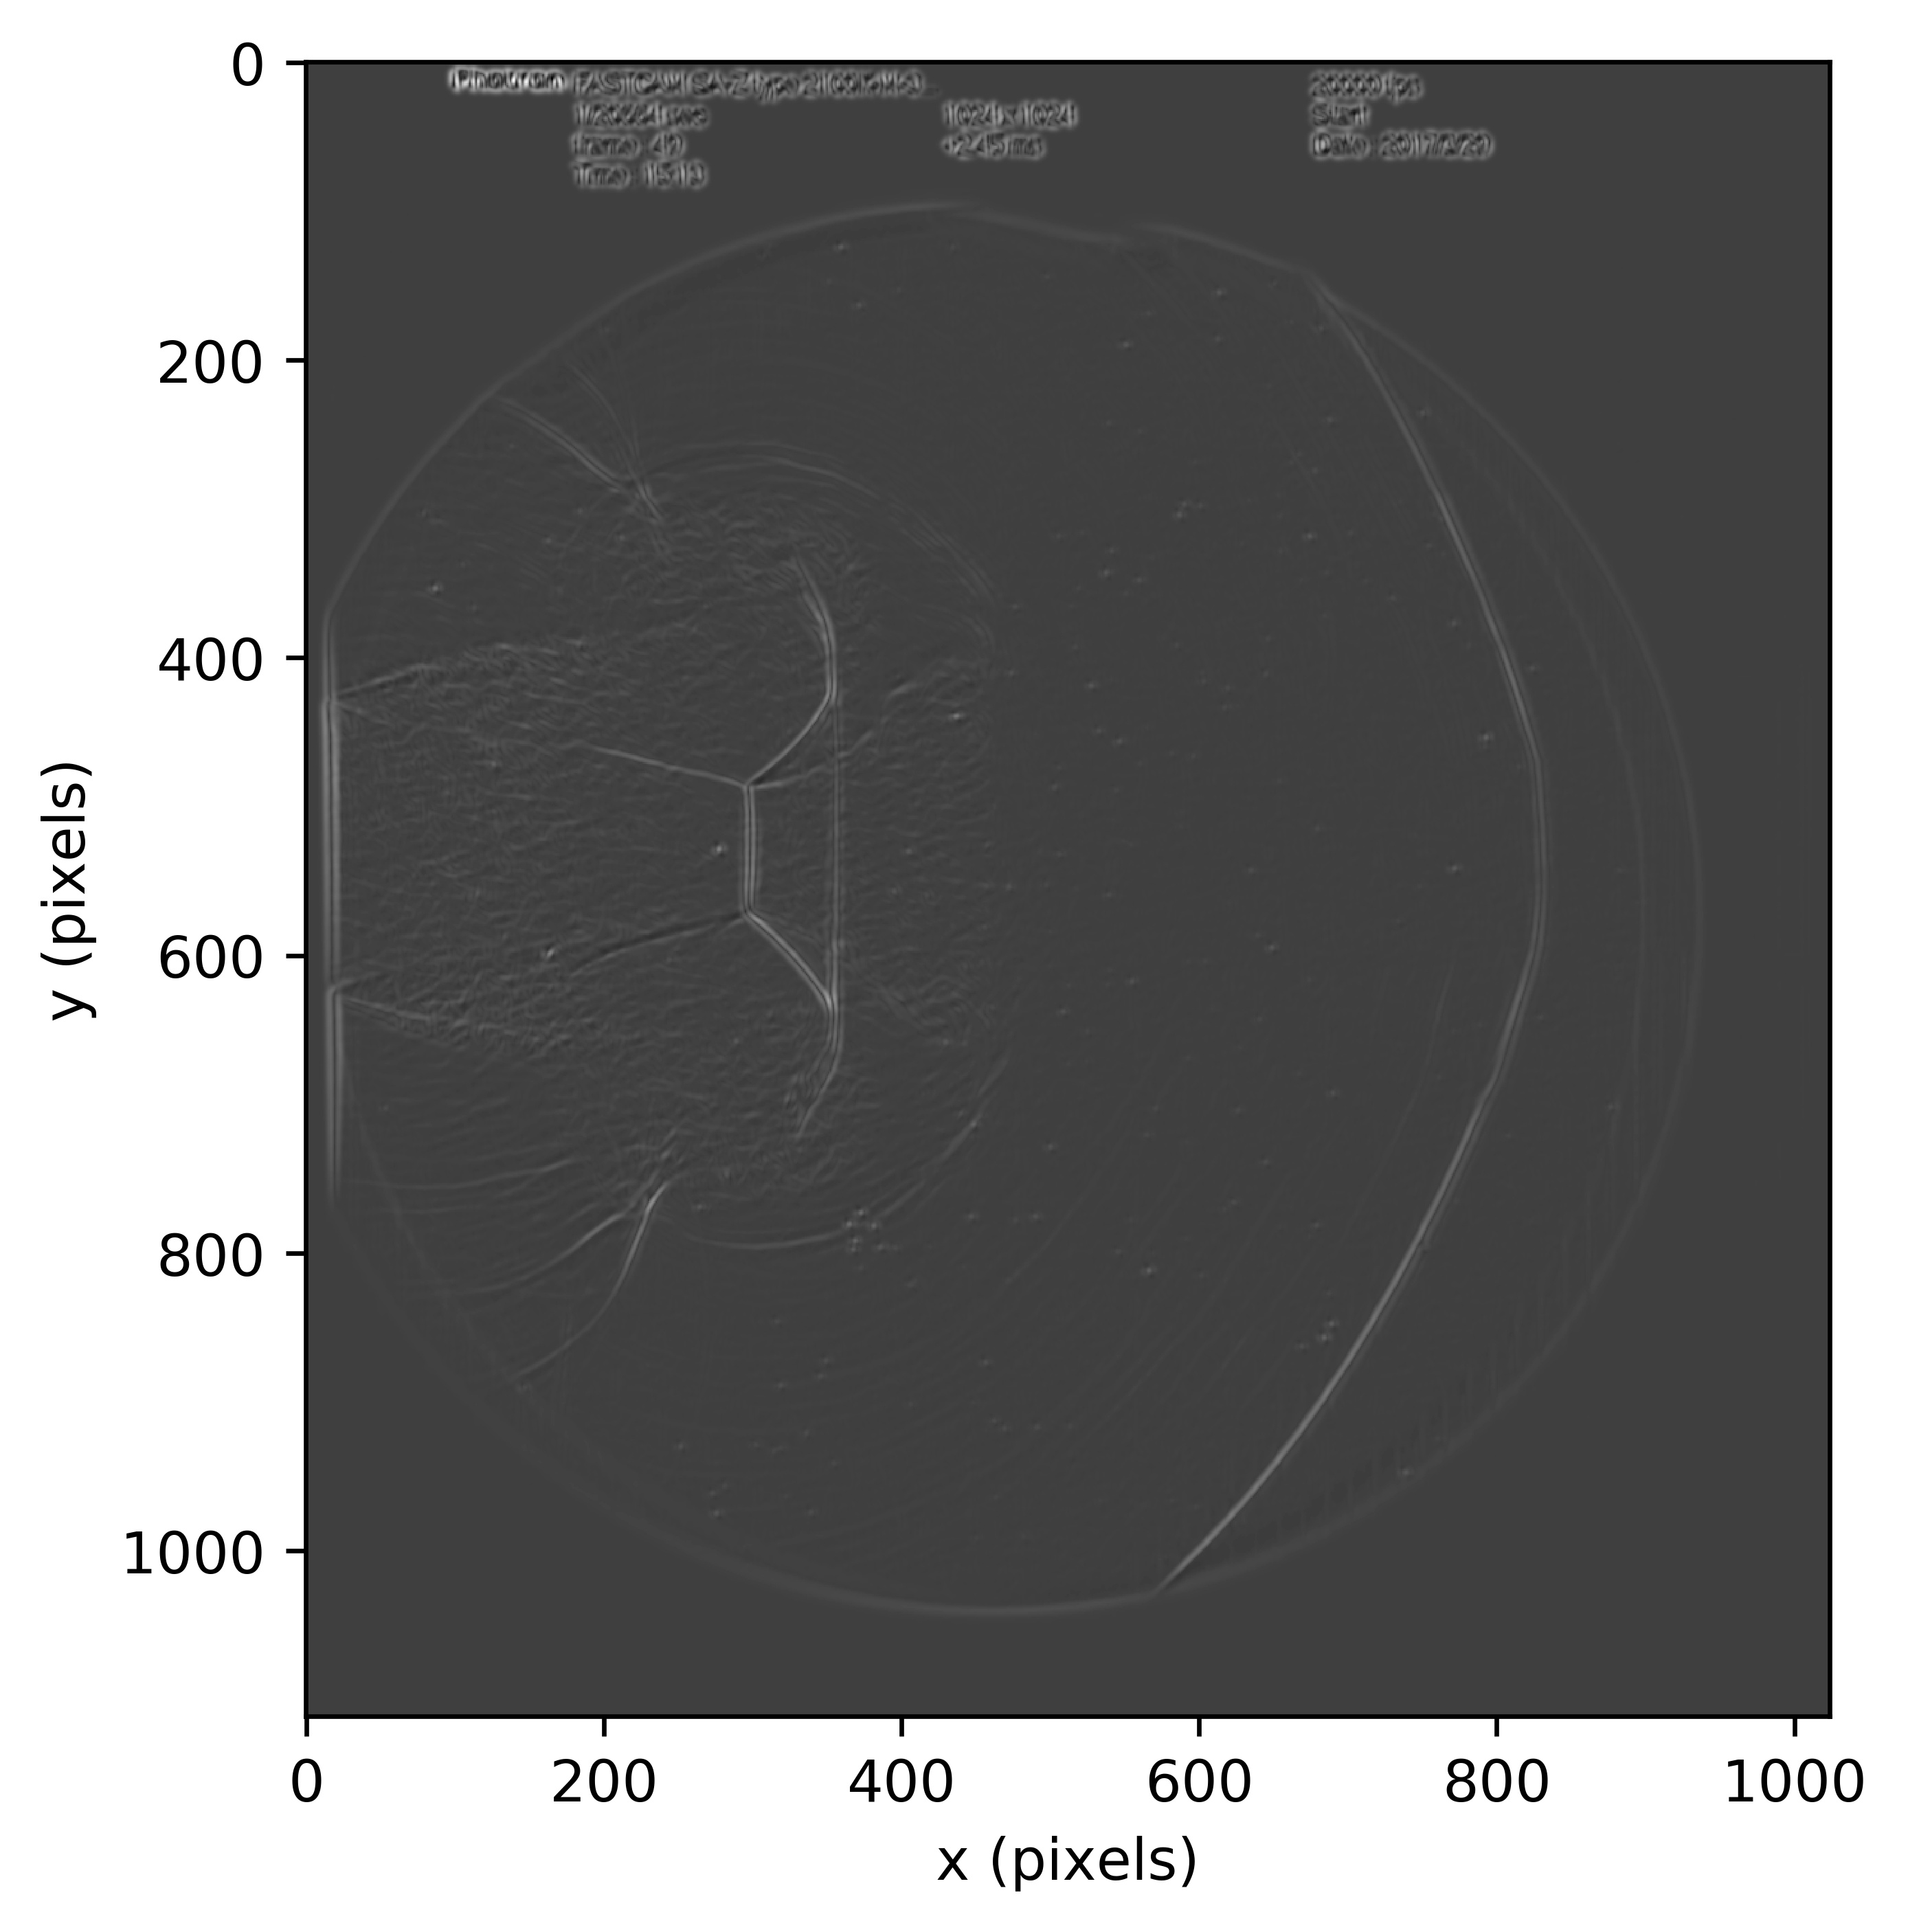
\includegraphics[width=0.48\textwidth]{sigma_2.jpg}}
  \caption{Second order convolution parameter.}
  \label{fig:hessian_img}
\end{figure}

\subsection{Morphology: Erosion}
Mathematical morphology contributes several operators to image processing, all derived from set theory concepts. These operators are particularly useful for the analysis of binary images with some applications to grey scale images. Morphological operators are capable of edge detection, noise removal, image enhancement, and image segmentation. Morphological erosion is the next step in the flow feature extraction pipeline. It requires an input image, taken from the Hessian detector, and a structuring element (also known as a kernel). For a grayscale image the intensity value is taken to represent height above a base pixel plane, as shown in Figure \ref{fig:erosion}. This 3-dimensional greyscale image represents a surface in 3-dimensional Euclidean space, the associated image surface coordinates are simply transformed to 3-dimensional Euclidean coordinates.

Morphological erosion sets a pixel at (i,j) to the minimum over all pixels in the neighborhood centered at (i,j). Erosion shrinks bright regions and enlarges dark regions.

In other words the erosion of a point is the minimum of the points in its neighborhood, with that neighborhood defined by the structuring element. In this way it is similar to many other kinds of image filters like the median filter and the gaussian filter.

\begin{figure}[H]
  \centering
  \subfloat[Input image .]{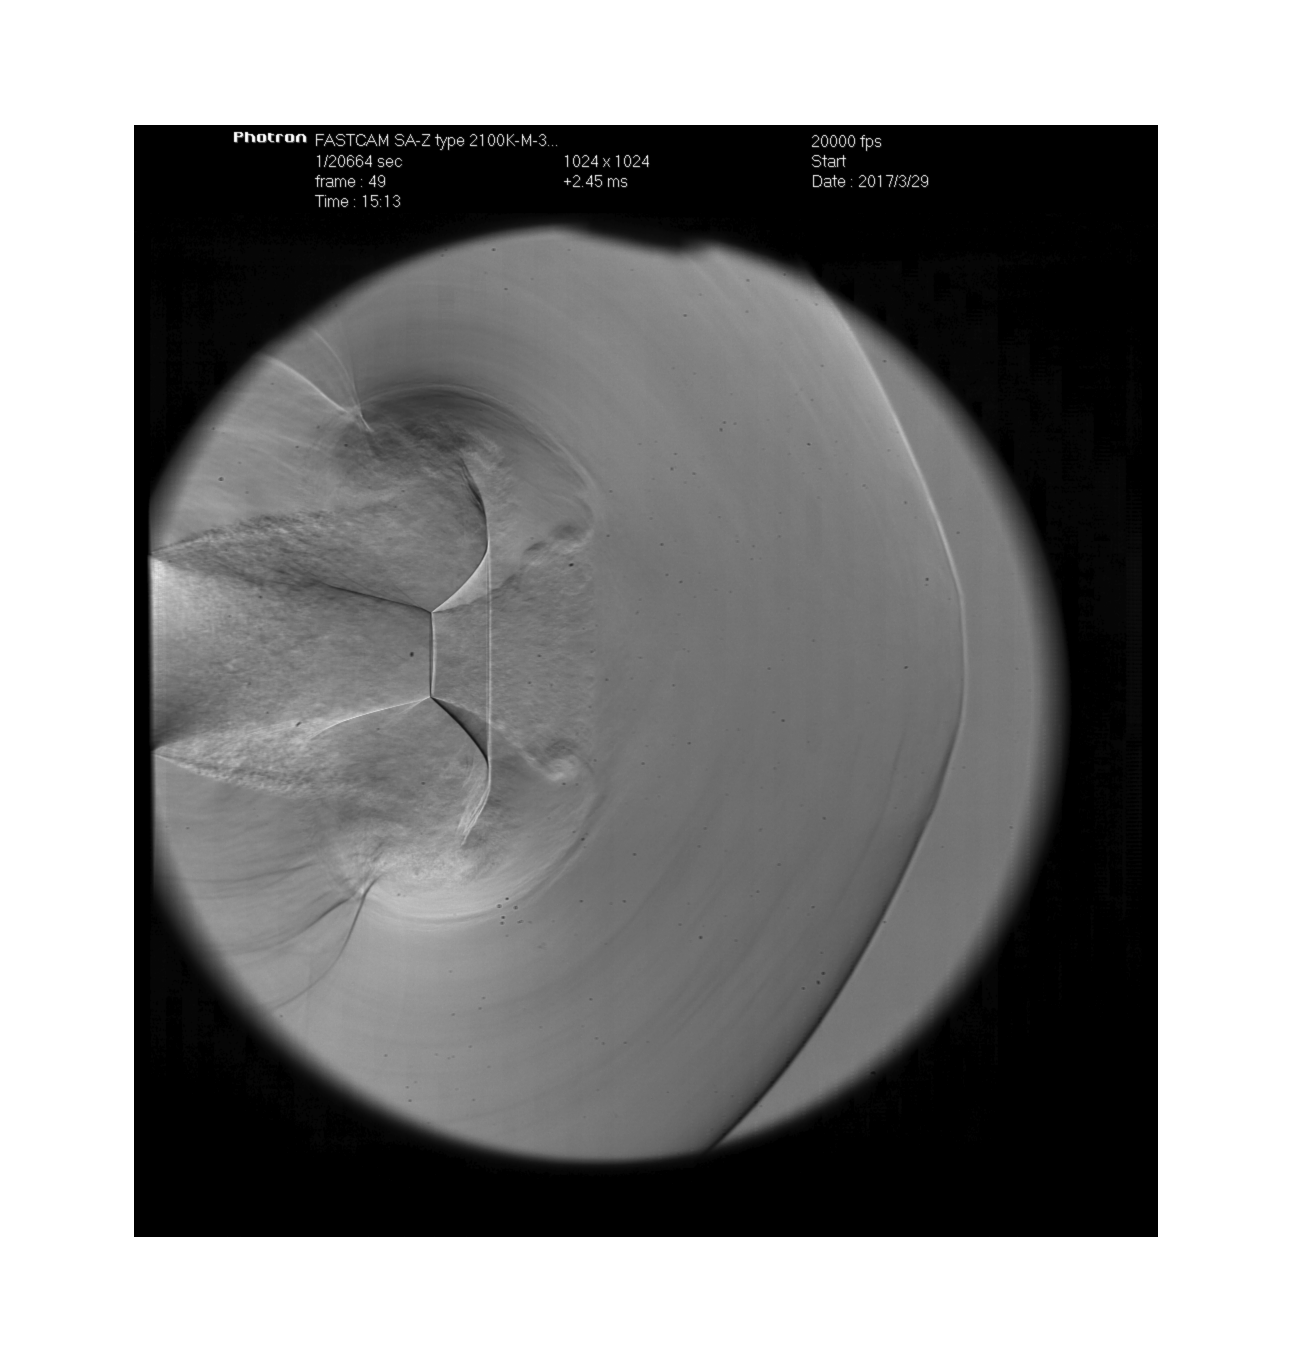
\includegraphics[width=0.48\textwidth]{vid89_frame50.png}}
  \hfill
  \subfloat[3-dimensional representation.]{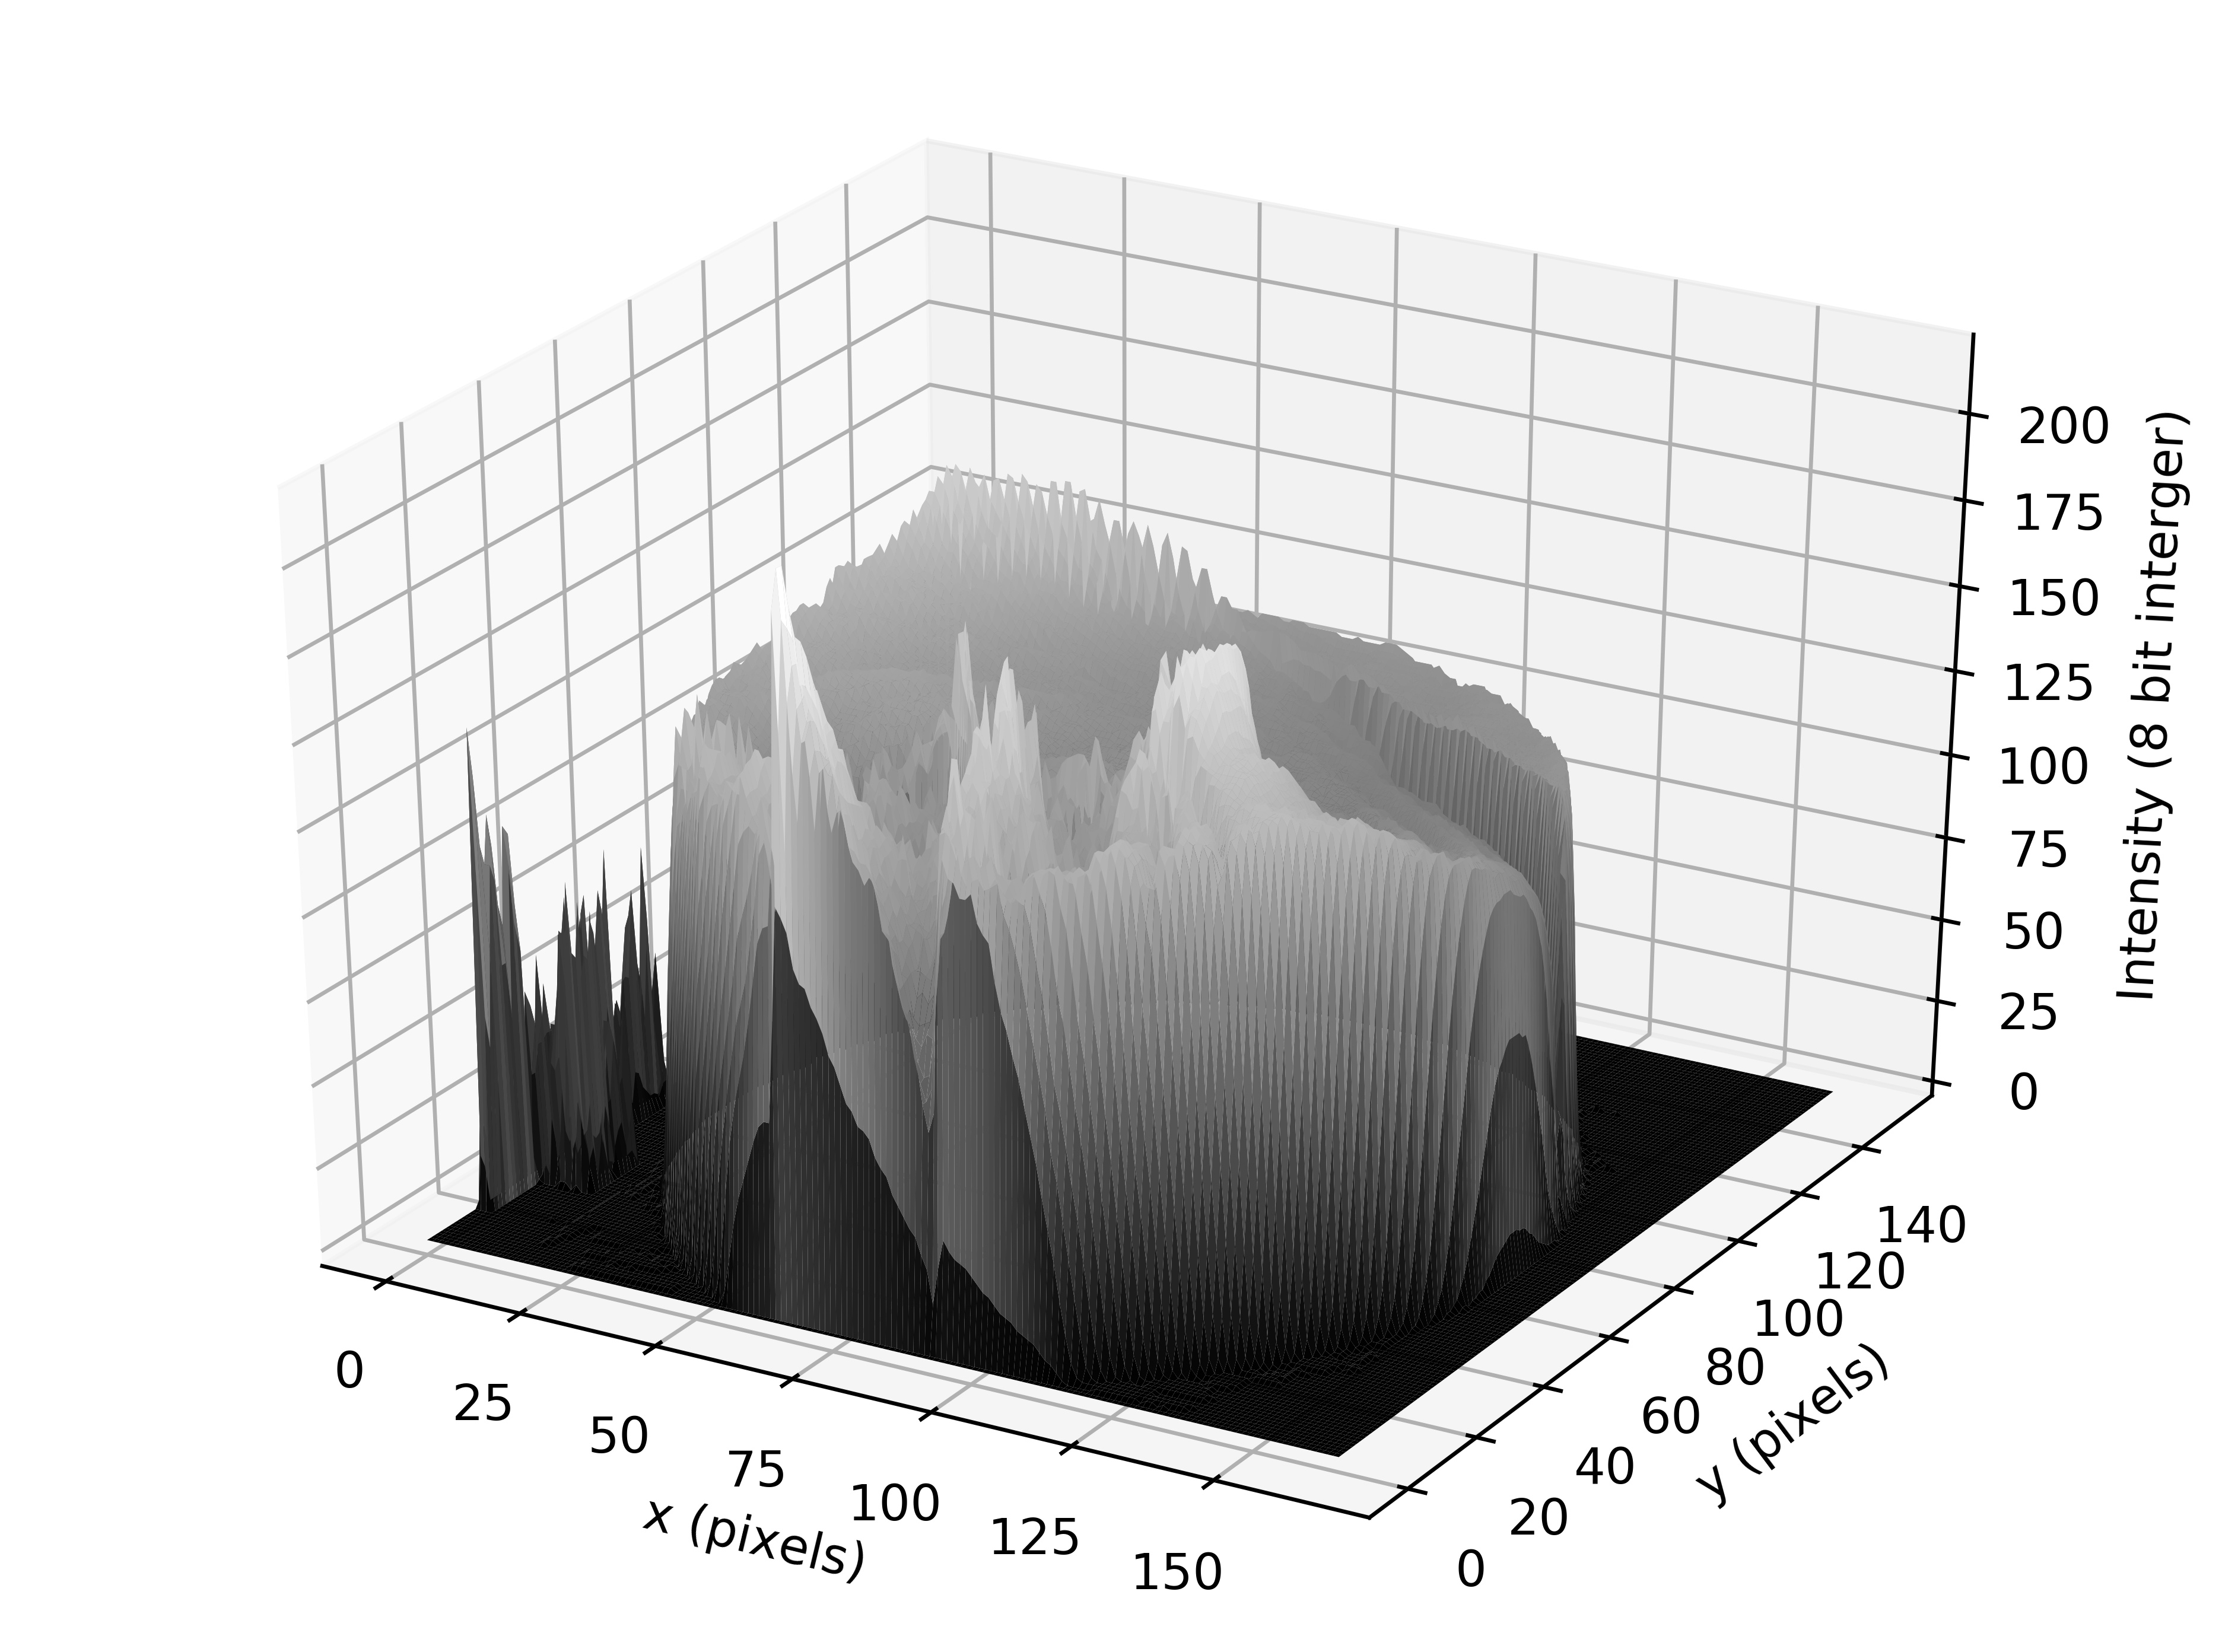
\includegraphics[width=0.48\textwidth]{3d_intensity.jpg}}
  \caption{Second order convolution parameter.}
  \label{fig:erosion}
\end{figure}



In grayscale morphology, images are functions mapping a Euclidean space or grid E into ${\displaystyle \mathbb {R} \cup \{\infty ,-\infty \}} {\mathbb  {R}}\cup \{\infty ,-\infty \}, where {\displaystyle \mathbb {R} } \mathbb {R}  is the set of reals, {\displaystyle \infty } \infty  is an element larger than any real number, and {\displaystyle -\infty } -\infty $ is an element smaller than any real number.
a structuring element (also known as a kernel).\\

Denoting an image by f(x) and the grayscale structuring element by b(x), where B is the space that b(x) is defined, the grayscale erosion of f by b is given by
\begin{equation}
(f\ominus b)(x)=\inf _{y\in B}[f(x+y)-b(y)]
\end{equation}



\subsection{Ranking Methods}
The next step of the flow feature extraction pipeline is to implement an intensity ranking method. Using the results from the morphological erosion operator, a normalised ranking method is utilised to threshold intensity values in the image array and reduce background noise. The normalised ranking method ranks the image array intensity as a normalised distribution, shown in Figure \ref{fig:dist}. Once a normalised distribution is acquired, the algorithm sets to zero all intensity values for a chosen percentile. Percentile ranges from the 90th up the 98th percentile were explored, this is shown in Figure \ref{fig:percentile}. All values within this range are suitable for extracting various flow features. The percentile used for each specific flow feature is stated in the relevant discussion section.

\begin{figure}[H] 
	\centering
	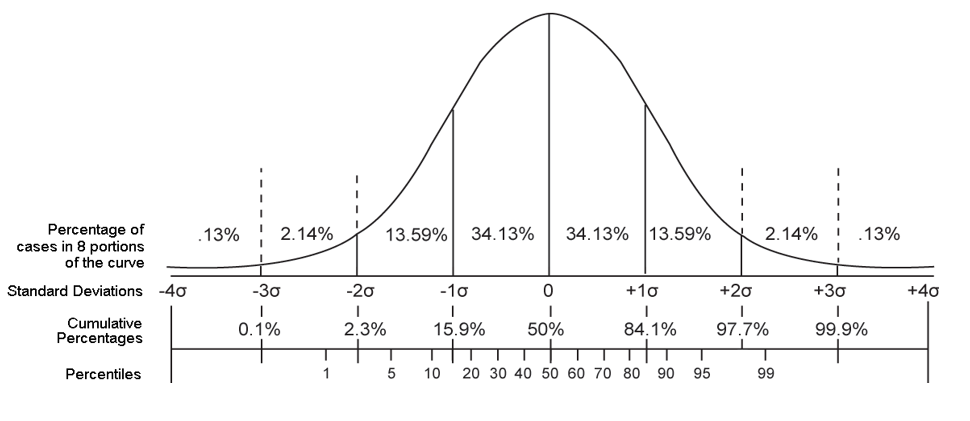
\includegraphics[width=1\textwidth]{dist.png} 
	\caption{Normal distribution \citep{brownlee1965statistical}.}
	\label{fig:dist}
\end{figure}


\subsection{Morphology: Small Object Removal}

\subsection{Connected Components}

\subsection{Hough Transforms}
\subsubsection{Straight Line}
\subsubsection{Probabilistic}


\newpage
\section{Results}

\newpage
\section{Discussion}

\newpage
\section{Conclusions and Recommendations}

\newpage
%\footnotesize
%\printbibliography
\bibliographystyle{apacite}
\bibliography{sample}

%----------------------------------------------------------------------------------------
\normalsize
\newpage

\appendix
\addcontentsline{toc}{section}{Appendix}

\section{Shock Facility} \label{app:facility}

\begin{figure}[H] 
	\centering
	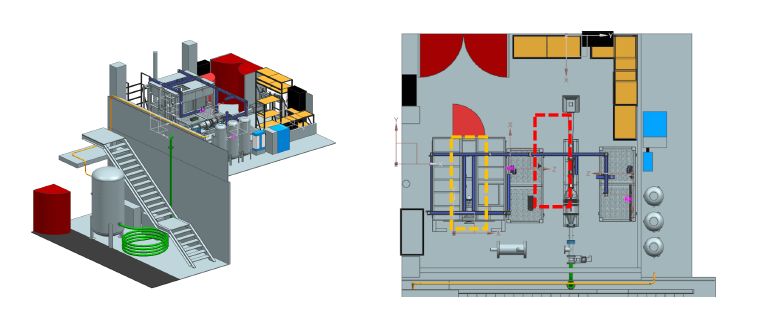
\includegraphics[width=1\textwidth]{fig10.PNG} 
	\caption{(Left): Isometric view of the LTRAC Shock Lab, with the shock tube facility stored under the
		shelving. (Right): Top view of the LTRAC Shock Lab, with the PIV (orange) and schlieren (red) sites
		highlighted.}
	\label{fig:10}
\end{figure}

\begin{figure}[H] 
	\centering
	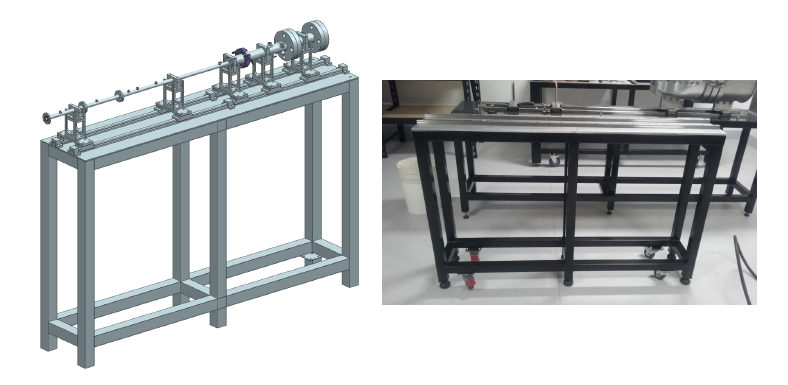
\includegraphics[width=1\textwidth]{fig8.PNG} 
	\caption{Isometric view of the design of the shock tube facility. (Right): Progress of the commission
		of the shock tube facility.}
	\label{fig:8}
\end{figure}

\section{Literature Comparison}
Initially, it is necessary to explore the literature and develop an understanding of the current comprehension of the flow characteristics governing supersonic transient jet impingement, and previous experimental test configurations. Section \ref{sec:background} undertakes an extensive review of previous literature, exploring the fluid dynamics and practical applications of supersonic impinging jets. Table \ref{tab1} details a summary for the research undertaken in previous literature, it's important to note all previous literature sources implement a plate diameter such that it can be considered infinite to the flow. Additionally, imaging results from the literature summarised in Table 1 is subsequently shown in appendix \ref{app:litresults}.

\begin{table}[h]
	\centering
	\caption{Literature Summary}
	\label{tab1}
	\resizebox{\textwidth}{!}{ 
		\begin{tabular}{@{}llllll@{}}
			\toprule
			Reference                                                                                                                           & \begin{tabular}[c]{@{}l@{}}Main\\ Research\\ Focus\end{tabular}                                                          & \begin{tabular}[c]{@{}l@{}}Imaging\\ Technique\end{tabular}                                            & \begin{tabular}[c]{@{}l@{}}Inner Shock\\ Tube\\ Diameter\end{tabular} & \begin{tabular}[c]{@{}l@{}}Incident\\ Mach\\ Number\end{tabular} & \begin{tabular}[c]{@{}l@{}}Impingement\\ Plate Distance\\ (inner diameter)\end{tabular}   \\ \midrule
			\multicolumn{1}{|l|}{\citep{minota1997shock}}                                                                                              & \multicolumn{1}{l|}{\begin{tabular}[c]{@{}l@{}}Shock-vortex \\ interaction in \\ the flow field\end{tabular}}            & \multicolumn{1}{l|}{Shadowgraph}                                                                       & \multicolumn{1}{l|}{40mm}                                             & \multicolumn{1}{l|}{1.35}                                        & \multicolumn{1}{l|}{0.4di}                                                                \\ \midrule
			\multicolumn{1}{|l|}{\citep{szumowski2000starting}}                                                                                              & \multicolumn{1}{l|}{\begin{tabular}[c]{@{}l@{}}Sound generation \\ upon impingement\end{tabular}}                        & \multicolumn{1}{l|}{Schlieren}                                                                         & \multicolumn{1}{l|}{65mm}                                             & \multicolumn{1}{l|}{1.14}                                        & \multicolumn{1}{l|}{2di}                                                                  \\ \midrule
			\multicolumn{1}{|l|}{\citep{murugan2010characteristics}}                                                                                              & \multicolumn{1}{l|}{\begin{tabular}[c]{@{}l@{}}Noise due to shock-\\ vortex interaction \\ and impingement\end{tabular}} & \multicolumn{1}{l|}{\begin{tabular}[c]{@{}l@{}}High-speed\\ smoke flow\\ visualisations.\end{tabular}} & \multicolumn{1}{l|}{64mm}                                             & \multicolumn{1}{l|}{1.31 - 1.55}                                 & \multicolumn{1}{l|}{4.7di}                                                                \\ \midrule
			\multicolumn{1}{|l|}{\citep{thangadurai2012experimental}}                                                                                              & \multicolumn{1}{l|}{\begin{tabular}[c]{@{}l@{}}Vortex ring\\ impingement\end{tabular}}                                   & \multicolumn{1}{l|}{\begin{tabular}[c]{@{}l@{}}High-speed\\ smoke flow\\ visualisations.\end{tabular}} & \multicolumn{1}{l|}{64mm}                                             & \multicolumn{1}{l|}{1.31 - 1.85}                                 & \multicolumn{1}{l|}{4.7di}                                                                \\ \midrule
			\multicolumn{1}{|l|}{\citep{mariani2013head}}                                                                                              & \multicolumn{1}{l|}{\begin{tabular}[c]{@{}l@{}}Vortex ring\\ impingement\end{tabular}}                                   & \multicolumn{1}{l|}{Schlieren}                                                                         & \multicolumn{1}{l|}{30mm}                                             & \multicolumn{1}{l|}{1.61}                                        & \multicolumn{1}{l|}{\begin{tabular}[c]{@{}l@{}}1.66di, \\ 3.33di, \\ 5.00di\end{tabular}} \\ \bottomrule
		\end{tabular}}
	\end{table}

\section{Shock Relations} \label{app:shock}
In this section, the relationship between the pressure of the flow behind the leading shock and the ambient pressure will be derived. Figure \ref{fig:shock} details pressure, temperature, and velocity relations for the shock tube.

\begin{figure}[H]
	\centering
	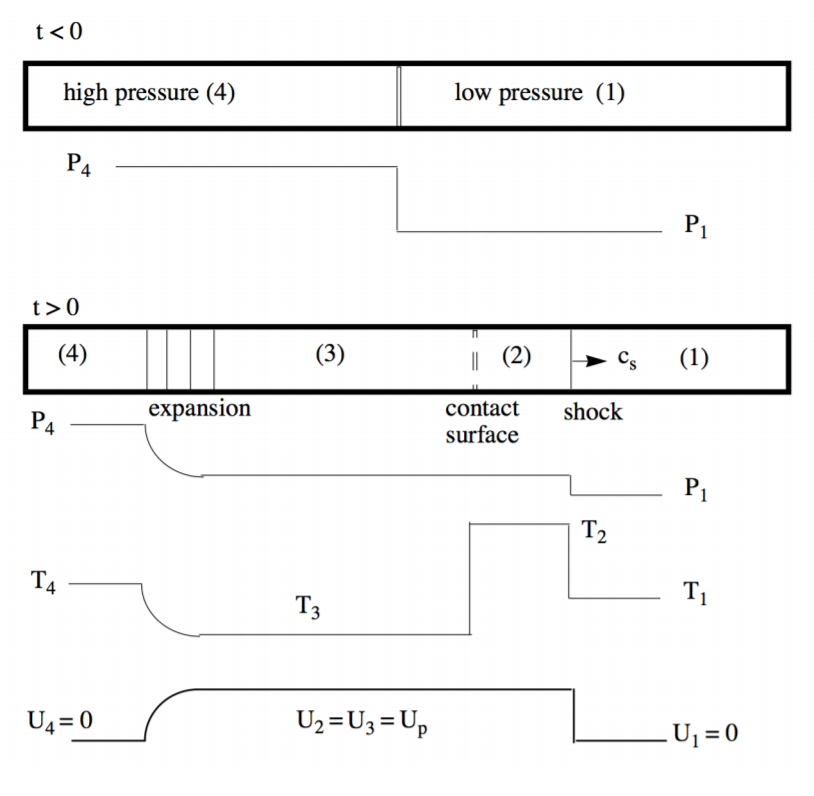
\includegraphics[scale=0.5]{figshock.png} 
	\caption{Shock tube flow regions: Region 1 is the flow ahead of the primary shock, region 2 is between contact surface and primary shock, region 3 is between tail of the expansion fan and contact surface, region 4 is ahead of the leading expansion wave \citep{cantwell2017}.}
	\label{fig:shock}
\end{figure}

In the following we will combine the results for expansion waves with normal shock relations to derive the so-called shock tube equation. The conditions at the contact surface are:
\begin{equation}
	P_2 = P_3 
\end{equation}
\begin{equation}
	U_2 = U_3 = U_p.
\end{equation}
\begin{center}
	where $U_2$ is the speed of the slug of gas set into motion by the opening of the diaphragm.
\end{center}
This is the effective piston speed of the fluid released by the diaphragm.

In a frame of reference moving with the shock wave the gas velocities are
\begin{equation}
U'_1 = -c_s
\end{equation}
\begin{equation}
U'_2 = -c_s + U_p
\end{equation}
and the shock jump conditions are

\begin{equation}
\frac{U'_2}{U'_1} = \frac{1+\frac{\gamma_1-1}{2}M_1^2}{\frac{\gamma_1+1}{2}M_1^2} 
\end{equation}
\begin{equation}
\frac{P_2}{P_1} = \frac{\gamma_1M_1^2-\frac{\gamma_1-1}{2}}{\frac{\gamma_1+1}{2}} 
\end{equation}
\begin{center}
	where $M_1 = c_s/a_1 = -U'_1/a_1$. Using the first relation, Equation 5 above, we can write
\end{center}

\begin{equation}
\frac{U'_2 - U'_1}{U'_1} = \frac{1 + \frac{\gamma_1-1}{2}M_1^2}{\frac{\gamma_1+1}{2}M_1^2} - 1 = \frac{1 - M_1^2}{\frac{\gamma_1+1}{2}M_1^2}
\end{equation}

The piston velocity is

\begin{equation}
U_p = U'_2 - U'_1 = U'_1\left(\frac{1 - M_1^2}{\frac{\gamma_1+1}{2}M_1\frac{-U'_1}{a_1}}\right) = a_1\left(\frac{M_1^2 - 1}{\frac{\gamma_1+1}{2}M_1}\right) 
\end{equation}

Note that $U_p$ is positive. Using the second relation, Equation 5, Equation 8 can be expressed in terms of the shock pressure ratio as 

\begin{equation}
U_p = a_1\left(\frac{P_2}{P_1} - 1\right)\left(\frac{2}{\gamma_1(\gamma_1 + 1)(P_2/P_1) + \gamma_1(\gamma_1 - 1)}\right)^{1/2}
\end{equation}

Equation 9 is the expression for the piston velocity derived using normal shock theory. Now lets work out an expression for the piston velocity using isentropic expansion theory. The velocity behind the expansion is

\begin{equation}
U_3 = U_p = \frac{2a_4}{\gamma_4 - 1}\left(1 - \frac{P_3}{P_4}^{\frac{\gamma_4 - 1}{2\gamma_4}}\right)
\end{equation}

Equate 9 and 10.

\begin{equation}
a_1\left(\frac{P_2}{P_1} - 1\right)\left(\frac{2}{\gamma_1(\gamma_1 + 1)(P_2/P_1) + \gamma_1(\gamma_1 - 1)}\right)^{1/2} = \frac{2a_4}{\gamma_4 - 1}\left(1 - \left(\frac{P_3}{P_2}\frac{P_2}{P_1}\frac{P_1}{P_4}\right)^{\frac{\gamma_4 - 1}{2\gamma_4}}\right)
\end{equation}

Using the following identity

\begin{equation}
\frac{P_3}{P_4}=\frac{P_3}{P_2}\frac{P_2}{P_1}\frac{P_1}{P_4}
\end{equation}

and noting that $P_3/P_2 = 1$ solve Equation 10 for $P_4/P_3 = 1$, substituting in $P_2/P_1$ from Equation 6. Simplifying, the result is the basic shock tube equation

\begin{equation} \label{shock_relation}
\frac{P_4}{P_1} = \frac{2\gamma_1M_1^2 - (\gamma_1 - 1)}{\gamma_1 + 1}\left(1 - \frac{\gamma_{4-1}}{\gamma_{1+1}}\frac{U_1}{U_4}\left(M_1 - \frac{1}{M_1}\right)\right)^{-2\gamma_4/\gamma_{4-1}}
\end{equation}
And given the specific gas information, for the driver helium, $\gamma_4 = 1.667$, and the driven air, $\gamma_1 = 1.4$. Taking the ambient air temperature $T_1 = 273.15K$, the relation in Equation \ref{shock_relation} can be shown in the Figure \ref{fig:gas_relation}. This figure highlights the relationship between the driver pressure ratio at 4, and the ambient pressure at 1, for a design incident Mach number. The figure also illustrates the reduced pressure ratio benefit of using a helium to air experiment in comparison to an air to air experiment. 

\section{Image Processing Algorithms} \label{app:code}

\section{Second Order Convolution Data} \label{app:hessian}
	

\end{document}
